\documentclass{report}


\usepackage[usenames,dvipsnames,svgnames,table]{xcolor} % Before listings
\usepackage{amsmath} % Better matrix environment
\usepackage{amssymb}
\usepackage[inline]{enumitem} % inline numbering and resume numbering
\usepackage{etoolbox} % If conditions
\usepackage{graphicx}
\usepackage{listings} % for code
\usepackage{nth}
\usepackage{hyperref}
\usepackage{cleveref} % Must be loaded after hyperref
\usepackage[font=small,labelfont=bf]{caption}
\usepackage{pgfplotstable}
\pgfplotsset{compat=1.10}
\usepackage{subcaption}
\usepackage{svg}
\usepackage{tikz}
\usepackage{tikz-qtree,tikz-qtree-compat} % Trees
\usepackage{url}
\usepackage{xkeyval}
\usepackage{floatrow} % center floats
\usepackage{relsize}
% \usepackage{arydshln} % Dashed lines in tables

% Image directory
\graphicspath{{images/intro/}}

\pdfoptionpdfminorversion=5

% Squiggly lines
\usetikzlibrary{decorations.pathmorphing}


% Node shapes
\usetikzlibrary{shapes,decorations}

% Coordinate calculation
\usetikzlibrary{calc}

% For charts
\usetikzlibrary{patterns}

% Arrowheads
\usetikzlibrary{arrows.meta}

% Cross-table arrows
\usetikzlibrary{matrix, positioning}

\newcommand{\VertexSet}{V}
\newcommand{\CellSet}{C}

\newcommand{\Visited}{V_{visited}}

% Adjacency relation
\newcommand{\AdjVV}{Adj_{\VertexSet\VertexSet}}

% Cardinality of
\newcommand{\card}[1]{\left\vert{#1}\right\vert}

% powerset of
\newcommand{\powerset}[1]{\mathcal P \left({#1}\right)}


% Tikz function: compute absolute position
% row, delta-sy, y-offset
\newcommand{\rctoxy}[3][3=0]{#1*#2 + #3}



% Line that can go anywhere, structured region or outside
\tikzset{%
    anywhere/.style={
		decorate,
		decoration={
		    snake,
		    segment length=4,
		    amplitude=.9,post=lineto,
		    post length=2pt
		}
	}
}

% Line that can only go outside the structured region
\tikzset{outside/.style={dotted}}


% Ellipsis
\tikzset{ellipsis/.style={loosely dotted}}

% Structured
\tikzset{structured/.style={}}


%% Node labelling functions

% row, col, rowoffset, coloffset
\newcommand{\plainlabelnode}[4]{
\pgfmathtruncatemacro{\rowlabel}{#1+#3}\pgfmathtruncatemacro{\collabel}{#2+#4}$n_{\rowlabel,\collabel}$}

% row, col, rowoffset, coloffset, column-variable
\newcommand{\varcollabelnode}[5]{
\pgfmathtruncatemacro{\row}{#1+#3}\pgfmathtruncatemacro{\col}{#2+#4}\pgfmathtruncatemacro{\colzero}{\col-1}\newcommand{\collabel}{\ifnumcomp{\colzero}{=}{0}{#5}{\ifnumcomp{\colzero}{>}{0}{#5+\colzero}{#5\colzero}}}$n_{\row,\collabel}$}

% row, col, rowoffset, coloffset, row-variable
\newcommand{\varrowlabelnode}[5]{\pgfmathtruncatemacro{\row}{#1+#3}\pgfmathtruncatemacro{\rowzero}{\row-1}\pgfmathtruncatemacro{\col}{#2+#4}\newcommand{\rowlabel}{\ifnumcomp{\rowzero}{=}{0}{#5}{\ifnumcomp{\rowzero}{>}{0}{#5+\rowzero}{#5\rowzero}}}$n_{\rowlabel,\col}$}


% row, col, rowoffset, coloffset, row-variable, col-variable
\newcommand{\varlabelnode}[6]{\pgfmathtruncatemacro{\row}{#1+#3}\pgfmathtruncatemacro{\rowzero}{\row-1}\pgfmathtruncatemacro{\col}{#2+#4}\pgfmathtruncatemacro{\colzero}{\col-1}\newcommand{\rowlabel}{\ifnumcomp{\rowzero}{=}{0}{#5}{\ifnumcomp{\rowzero}{>}{0}{#5+\rowzero}{#5\rowzero}}}\newcommand{\collabel}{\ifnumcomp{\colzero}{=}{0}{#6}{\ifnumcomp{\colzero}{>}{0}{#6+\colzero}{#6\colzero}}}$n_{\rowlabel,\collabel}$}



\pgfkeys{/tikz/.cd,% to set the path
  rows/.get=\krows,
  rows/.store in=\krows,
  cols/.get=\kcols,
  cols/.store in=\kcols,
  rowoffset/.initial=0,
  rowoffset/.get=\krowoffset,
  rowoffset/.store in=\krowoffset,
  coloffset/.initial=0,
  coloffset/.get=\kcoloffset,
  coloffset/.store in=\kcoloffset,
  labeler/.get=\klabeler,
  labeler/.store in=\klabeler,
  labelerA/.get=\klabelerA,
  labelerA/.store in=\klabelerA,
  labelerB/.get=\klabelerB,
  labelerB/.store in=\klabelerB,
  labelerC/.get=\klabelerC,
  labelerC/.store in=\klabelerC,
  labelerD/.get=\klabelerD,
  labelerD/.store in=\klabelerD,
  northborder/.initial=outside,
  northborder/.get=\knorthborder,
  northborder/.store in=\knorthborder,
  southborder/.initial=outside,
  southborder/.get=\ksouthborder,
  southborder/.store in=\ksouthborder,
  eastborder/.initial=outside,
  eastborder/.get=\keastborder,
  eastborder/.store in=\keastborder,
  westborder/.initial=outside,
  westborder/.get=\kwestborder,
  westborder/.store in=\kwestborder,
}

%% Draws a grid - num rows, num cols, row offset, col offset
\newcommand{\drawgrid}[1]{{
     \tikzset{#1}


	\newcommand{\maxrows}{\krows}
	\newcommand{\maxcols}{\kcols}
	\newcommand{\rowoffset}{\krowoffset}
	\newcommand{\coloffset}{\kcoloffset}
	% Argument is a function: r,c -> node label
	\newcommand{\labeler}{\klabeler}

	\foreach \row in {1,...,\maxrows} {
		\pgfmathsetmacro{\ypos}{-2 * \row + \rowoffset}
		\pgfmathtruncatemacro{\prevrow}{\row - 1}

		\foreach \col in {1,...,\maxcols} {
			\pgfmathsetmacro{\xpos}{2 * \col + \coloffset}
			\pgfmathtruncatemacro{\prevcol}{\col - 1}
			\newcommand{\thisnode}{(n \row \space \col)}

			% Get node label
			\ifstrempty{\klabelerA}{
				\newcommand{\nodelabel}{\labeler{\row}{\col}}
			}
			\ifstrempty{\klabelerB} {
				\newcommand{\nodelabel}{\labeler{\row}{\col}{\klabelerA}}
			}
			\ifstrempty{\klabelerC} {
				\newcommand{\nodelabel}{\labeler{\row}{\col}{\klabelerA}{\klabelerB}}
			}
			\ifstrempty{\klabelerD} {
				\newcommand{\nodelabel}{\labeler{\row}{\col}{\klabelerA}{\klabelerB}{\klabelerC}}
			}
			{
				\newcommand{\nodelabel}{\labeler{\row}{\col}{\klabelerA}{\klabelerB}{\klabelerC}{\klabelerD}}
			}
			% Create node
			\node (n \row \space \col) at (\xpos,\ypos) {\nodelabel};

			% Line from node to the previous horizontal node
			\ifnumcomp{\col}{>}{1} {
				\draw (n \row \space \prevcol) -- \thisnode;
			}

			% Line from node to the previous vertical node
			\ifnumcomp{\row}{>}{1} {
				\draw (n \prevrow \space \col) -- \thisnode;
			}


			% West border lines
			\ifnumcomp{\col}{=}{1} {
				\draw[\kwestborder] \thisnode -- (\xpos-1, \ypos);
			}
			% East border lines
			\ifnumcomp{\col}{=}{\maxcols} {
				\draw[\keastborder] (\xpos+1, \ypos) -- \thisnode;
			}

			% North border lines
			\ifnumcomp{\row}{=}{1} {
				\draw[\knorthborder] \thisnode -- (\xpos, \ypos+1);
			}
			% South border lines
			\ifnumcomp{\row}{=}{\maxrows} {
				\draw[\ksouthborder] (\xpos, \ypos-1) -- \thisnode;
			}
		}
	}
}}
\pgfkeys{/tikz/.cd,% to set the path
  num/.get=\knum,
  num/.store in=\knum,
  rowoffset/.initial=0,
  rowoffset/.get=\krowoffset,
  rowoffset/.store in=\krowoffset,
  coloffset/.initial=0,
  coloffset/.get=\kcoloffset,
  coloffset/.store in=\kcoloffset,
}


%% Draws a row of vertical ellipses - num cols, row offset, col offset
\newcommand{\drawellipsisrow}[1]{{
	\tikzset{#1}

	\newcommand{\numellipses}{\knum}
	\newcommand{\rowoffset}{\krowoffset}
	\newcommand{\coloffset}{\kcoloffset}

	\foreach \col in {1,...,\numellipses} {
		\pgfmathsetmacro{\xpos}{2 * \col + \coloffset}
		\pgfmathsetmacro{\ypos}{\rowoffset}

		\draw[ellipsis] (\xpos, \ypos) -- (\xpos, \ypos-1);
	}
}}



\pgfkeys{/tikz/.cd,% to set the path
  num/.get=\knum,
  num/.store in=\knum,
  rowoffset/.initial=0,
  rowoffset/.get=\krowoffset,
  rowoffset/.store in=\krowoffset,
  coloffset/.initial=0,
  coloffset/.get=\kcoloffset,
  coloffset/.store in=\kcoloffset,
}


%% Draws a column of horizontal ellipses - num rows, row offset, col offset
\newcommand{\drawellipsiscol}[1]{{
	\tikzset{#1}

	\newcommand{\numellipses}{\knum}
	\newcommand{\rowoffset}{\krowoffset}
	\newcommand{\coloffset}{\kcoloffset}

	\foreach \row in {1,...,\numellipses} {
		\pgfmathsetmacro{\xpos}{\coloffset}
		\pgfmathsetmacro{\ypos}{-2 * \row + \rowoffset}

		\draw[ellipsis] (\xpos, \ypos) -- (\xpos+1, \ypos);
	}
}}

\begin{document}

\chapter{Introduction}
Scientific computing is a large research branch touching on various areas in the scientific community as well as in various industries. An integral part of it is concerned with algorithms and techniques which operate on a mesh representation of a model, typically modelling physical phenomena such as the motion of fluids. SEE
% [Flow simulation and high performance computing, 1996a T. Tezduyar, http://www.tafsm.org/PUB_PRE/jALL/j63-CM96.pdf]
. SEE
% [http://www.sv.vt.edu/classes/MSE2094_NoteBook/97ClassProj/num/widas/history.html]
for a good introduction on finite element analysis.


Various methods of representing meshes exist, including X, Y, and Z
% [http://en.wikipedia.org/wiki/Polygon_mesh#Representations]
. Representations typically rely on encoding some form of explicitly-defined mapping between mesh elements. This can be represented straightforwardly as a flat array, with the array indices representing elements in the source set, and each value being one or more values representing one or more elements in the destination/target set. We focus our attention to the case where the number of target elements mapped to from each source element is constant. Such a map is known as a constant-arity map.

Consider for instance a quadrilateral mesh with two element sets \texttt{C} and \texttt{V}, representing the set of cells and vertices, respectively.
We can define a dat of coordinates, which associates the set each vertex $v \in V$ with a coordinate pair $(x_v, y_v)$, representing its position in 2D space.

We can then define an adjacency map (of constant arity 4) from cells to vertices:

\texttt{$C \rightarrow Node^4$}

Now consider an operation over this mesh, which performs a computation for each cell $c \in C$ as a function of its adjacent nodes ${n | n \in Map[c]}$, for instance computing the area of the cell. In particular consider the chain of memory access indirections and the resulting memory access patterns:

%
%             |   |             |   |
%             |   |  /----n3--->|   | -> (x_1, y_1)
%             |   | /           |   |
% cell_id ->  |   |/------n1--->|   | -> (x_4, y_4)
%             |   |\            |   |
%             |   | \-----n4--->|   | -> (x_5, y_5)
%             |   |  \          |   |
%             |   |   \---n2--->|   | -> (x_12, y_12)
%             |   |             |   |
%             |   |             |   |
%             |   |             |   |
%           cell2nodes         node2coordinate

Notice that proximate (or indeed adjacent) nodes in the mesh need not exhibit a uniform memory access pattern. This is detrimental to performance for various reasons.
1. They do not exhibit spatial locality, a property which most modern CPU caches bank on to attain higher performance in IO bound applications, which may manifest through decisions regarding cache replacement strategies or data pre-fetching.
2. Looking up addresses, as opposed to computing them directly, will typically prohibit or limit the scope of compiler-performed optimizations, not least vectorizations.

Numerous strategies have been devoted to deal with this problem, notably applying a space filling curve to obtain a more favourable numbering, with closer elements tending to have closer numberings. While the space filling curve most certainly improves cache locality, it does not make use more obvious structure that may exist. A mesh that is irregular and unstructured on the whole may contain subregions of high regularity and uniform structure, whose regularity/uniformity may be locally exploitable in a more direct manner, for potentially higher gain!


We present Crystal mesh, a group of algorithms for \emph{extracting} regions of regularity in a mesh, reorganizing the mesh to \emph{expose} said structure in order to enable efficient \emph{exploitation}.
In particular, we present and evaluate an implementation for extracting and exposing structure in quadrilateral meshes on various examples, and evaluate a 33\% performance improvement achieved by exploiting the structure on the airfoil computation.


\chapter{Background}
Before continuing further, we introduce briefly the main notions required to appreciate this work.

\section{The mathematical mesh model}

Meshes often model physical objects and phenomena. This is typically achieved through the discretization of a continuous model, such as the surface or volume of an object, in order to approximate its physical properties to a desired degree of precision.
\par

The mesh model consists of a hierarchy of elements, which may include a subset the following:
\begin{itemize}
\item Polyhedra such as cubes or tetrahedrons
\item Polygons \emph{(also referred to as cells or faces)} such as triangles and quadrilaterals
\item Edges
\item Vertices \emph{(also referred to as nodes)}
\end{itemize}

\includesvg[width=\imagewidth, svgpath=images/background/]{mesh-elements}

Each element in the above hierarchy is built-up from those below it. Thus, a polyhedron is assimilated by a set of polygons, a polygon is composed by a set of edges, and an edge joins two vertices.


\subsection{Geometry vs topology}
There is a key distinction to make between the geometric and topological properties of a mesh.

Since meshes model a physical reality, the elements of a mesh may be spatially embedded: vertices are associated with points in space, and edges are formed as segments joining their two vertices. This affects \emph{geometric} properties of the mesh, such as its surface area or volume.

On the other hand, the hierarchy of elements described above induces a mesh topology. This describes the connectedness of the mesh, that is to say how elements relate to one another. For instance, we may describe two vertices sharing an edge as \emph{adjacent}, or two cells being sharing an edge as being \emph{incident} on that edge.
\par
In this work we concern ourselves solely with the topological structure of meshes, treating its geometry as arbitrary data that is associated with its respective elements (the position of a vertex for instance). Figure~\ref{fig:same-topology} illustrates the difference between the two concepts.

\begin{figure}
    \includesvg[width=\imagewidth, svgpath=images/background/]{same-topology}
    \caption{Despite having completely different geometric shapes and properties, the two meshes are topologically equivalent. The labels indicate corresponding vertices.}
    \label{fig:same-topology}
\end{figure}




\subsection{Manifold meshes}
A mesh is a manifold if the following properties hold:
\begin{enumerate}
\item All edges are adjacent to either one or two faces.

\item All faces meeting at a given vertex must form either an open or a closed fan around that vertex (Figure~\ref{fig:open-closed-fans}).
\end{enumerate}

% Open and closed fans
\begin{figure}
    \sidebyside
        {\includesvg[width=\imagewidth, svgpath=images/background/]{closed-fan}
        \caption{A closed fan}}
        {\includesvg[width=\imagewidth, svgpath=images/background/]{open-fan}
        \caption{An open fan}}
    \caption{}
    \label{fig:open-closed-fans}
\end{figure}

Figure~\ref{fig:non-manifolds} demonstrates examples of non-manifold meshes. In this work we consider manifold meshes exclusively, and future mentions of `mesh' shall implicitly refer to manifold meshes.

% Non-manifolds
\begin{figure}
    \sidebysidefour
    {\includesvg[width=\textwidth, svgpath=images/background/]{bad-fan}
        \caption{Faces incident on a vertex which do not form a continuous fan}}
    {\includesvg[width=\textwidth, svgpath=images/background/]{bad-fan2}
        \caption{An extra face that breaks off from the otherwise closed fan}}
    {\includesvg[width=\textwidth, svgpath=images/background/]{bad-multi-edge}
        \caption{More than two faces incident on a single edge}}
    {\includesvg[width=\textwidth, svgpath=images/background/]{bad-no-edge}
        \caption{An edge with no incident faces}}

    \caption{Examples of non-manifold meshes.}
    \label{fig:non-manifolds}
\end{figure}





\section{The mesh data structure}

We describe how a mesh model is manifest at the data structure level. There are three general component types can be identified:
\begin{itemize}
\item Entity sets
\item Associative data
\item Relations between two entity sets
\end{itemize}

In the following sections, the examples shall refer to the mesh depicted in figure~\ref{fig:example-mesh}.

\begin{figure}
    \includesvg[width=\textwidth, svgpath=images/background/]{mesh-data-structure}
    \caption{Example mesh with labelled elements.}
    \label{fig:example-mesh}
\end{figure}


\subsection{Entity sets}
Each set represents a certain type of entity in the mesh, such as vertices or cells. Each element in a set is associated with a unique identifier. Integers are a common choice as an identifier for a couple of reasons:
\begin{itemize}
\item They need not be enumerated explicitly. All we need is the set cardinality and a starting index.
\item They are convenient for direct-indexed array accesses, as well as for more general indexing methods.
\end{itemize}

See figure~\ref{fig:entity-sets} for examples.

\begin{figure}
    \includesvg[width=\textwidth, svgpath=images/background/]{entity-sets}
    \caption{The entity sets of the mesh in figure~\ref{fig:example-mesh}. These are (from left to right) the vertices, edges, and cells.}
    \label{fig:entity-sets}
\end{figure}


\subsection{Associative data}
Arbitrary data which is associated with elements of a particular entity set. For instance, spatial coordinates associated with each vertex. A typical representation is a flat array indexed by element identifier.
This is the data over which we perform our computations and ultimately care about. Everything else is incidental.
See figure~\ref{fig:associative-data} for an example.

\begin{figure}
    \includesvg[width=\textwidth, svgpath=images/background/]{associative-data}
    \caption{Coordinate data associated with the vertices of the mesh in figure~\ref{fig:example-mesh}.}
    \label{fig:associative-data}
\end{figure}


\subsection{Relation maps between two entity sets}
Entity sets may have relations defined between them, a mapping from an element in a source set to one or more corresponding elements in the destination set. For instance, we may have an adjacency relation from the vertex set to itself, or an inclusion relation from the cell set to the vertex set.
In a general unstructured mesh these relations must be explicitly stored, typically as an array indexed by the source element's identifier.
See figure~\ref{fig:relation} for an example.

\begin{figure}
    \includesvg[width=\textwidth, svgpath=images/background/]{relation}
    \caption{Inclusion relation from cells to vertices, as depicted in the mesh of figure~\ref{fig:example-mesh}.}
    \label{fig:relation}
\end{figure}




\section{The core-computation contract}
Given a mesh model and its underlying representation, computation logic provided by an external user is to be executed. We refer to this as the \emph{core-computation} so as to disambiguate it from other incidental processing, such as structure detection.
Our contract to the user is described in what follows.

\subsection{Given: operating set}
We are given an entity set over which to operate, for example the set of edges or the set of cells. We refer to this entity set as the \emph{operating set}. The core-computation consists of executing a computation for each element of the operating set. This is analogous to the \emph{map} phase of the MapReduce programming model~\cite{dean2008mapreduce}, though we restrict our usage of the term \emph{map} to refer to relation maps.

\subsection{Given: relation-map tree}
We are given a tree structure defining which relation maps to use and how to access them. This is best explained through an example, illustrated in figure~\ref{fig:relation-tree}. The core-computation will, for each element in the operating set, gather all indexing variables as described by the relation-map tree.


\begin{figure}
    %% Key icon
    \newcommand{\keyicon}{\includesvg[width=6pt, svgpath=images/background/]{key}}

    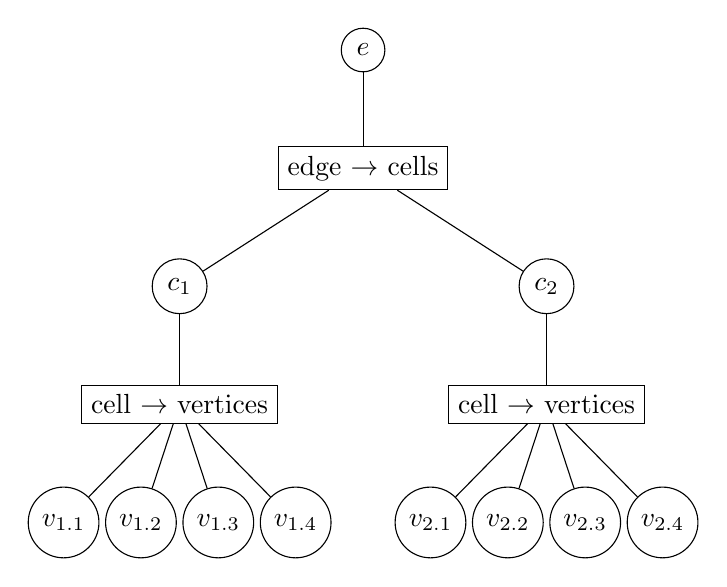
\begin{tikzpicture}[every tree node/.style={draw,circle},
        level distance=1.5cm,
        edge from parent path={(\tikzparentnode) -- (\tikzchildnode)}]

    \tikzset{level 2/.style={sibling distance=0.8cm}}

    \Tree
    [.{$e$}
        \edge node[auto=right] {\keyicon};
        [.\node[rectangle] {edge $\rightarrow$ cells};
            [.{$c_1$}
                \edge node[auto=right] {\keyicon};
                [.\node[rectangle] {cell $\rightarrow$ vertices};
                    [.$v_{1.1}$ ]
                    [.$v_{1.2}$ ]
                    [.$v_{1.3}$ ]
                    [.$v_{1.4}$ ]
                ]
            ]
            [.{$c_2$}
                \edge node[auto=right] {\keyicon};
                [.\node[rectangle] {cell $\rightarrow$ vertices};
                    [.$v_{2.1}$ ]
                    [.$v_{2.2}$ ]
                    [.$v_{2.3}$ ]
                    [.$v_{2.4}$ ]
                ]
            ]
        ]
    ]
    \end{tikzpicture}
    \caption{
    In this example, we consider a core-computation operating over the edge set, with $e$ being the indexing variable into the edge set.
    The edge $\rightarrow$ cells map is indexed by $e$ to obtain the the two cells $c_1$ and $c_2$ incident on the edge $e$. The cell $\rightarrow$ vertices map is then indexed by both $c_1$ and $c_2$ to obtain their respective vertices. The key symbol denotes indexing into the map below, using the indexing variable above.
    }
    \label{fig:relation-tree}
\end{figure}


\subsection{Given: kernel function}
\label{subsec:given-kernel-function}
We are given a kernel function specifying the computation logic, which is applied to each element in the operating set. It takes as arguments all gathered indexing variables, including that of the current element, and it has read and write access to the mesh's associated data. The access pattern of a kernel function is similar to that of a stencil computation, as defined by~\cite{tang2011pochoir}:
\begin{quote}
A stencil computation repeatedly updates each point of a d-dimensional grid as a function of itself and its near neighbours.
\end{quote}
As we define it, however, kernel functions are in fact more general than a stencil computation, as they access neighbouring elements across different operating sets.


The kernel function is applied to the operating set elements in no particular order; the indexing variables, however, are passed to the kernel in some known order, typically in the order stored in the relation-map.


\subsection{Expected operation}
Given all the above, a core-computation is then performed as follows:
\begin{enumerate}
\item Iterate over the elements of the operating set, in no particular order.
\item For each element iterated over:
    \begin{enumerate}
    \item Gather any indexing variables as defined by the relation-map tree. This may involve indexing variables obtained through a chain of relation-maps.
    \item Call the kernel function, passing the gathered indexing variables in some known order. The kernel function may access any associative data using these indexing variables.
    \end{enumerate}
\end{enumerate}



\section{Background on airfoils}
%% TODO CROSS REFERNCE to benchmarks
While not strictly needed for understanding our work, we nonetheless describe briefly airfoils and their function to offer a broader context. Much of this section was adapted from~\cite{abbott2012theory}, \cite{kuethe1986foundations} and~\cite{boeing2014airfoil}. Our description is nonetheless undoubtedly an overly simplistic one, and we would recommend that the aforementioned literature be sought for a fuller picture.

An airplane achieves flight by creating a lower air pressure over the wing (\emph{the upper surface}) whilst maintaining a higher air pressure below the wing (\emph{the lower surface}). The exact way in which this is achieved is characteristic of the wing shape as well as other factors. The pressure differential causes air in the lower surface to push towards the upper surface, creating a lift force. If the lift force is sufficient to counteract the gravitational force, the airplane flies.

An airfoil is the two-dimensional cross-section \emph{shape} of a wing. They are used to model the hydrodynamics (fluid motion) surrounding a particular wing shape in different contexts, including the velocity and angle of motion (known as the \emph{angle of attack}). Figure~\ref{fig:airfoil-crosscut} shows how the cross-section is taken, as well as the modelled air flow.

\begin{figure}
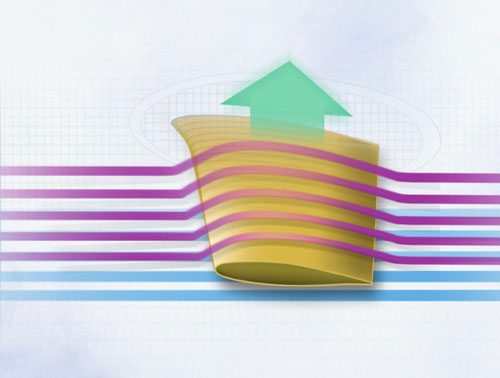
\includegraphics[width=\imagewidth]{images/background/airfoil_crosscut.jpg}
    \caption{The cross-section used to obtain the airfoil shape. Incoming air flow is split between the upper surface (purple) and the lower surface (blue). The image was obtained from~\cite{boeing2014airfoil}.}
    \label{fig:airfoil-crosscut}
\end{figure}


In 1929, the National Advisory Committee for Aeronautics (NACA) began to study various airfoils. They developed families of airfoil constructions parametrized by various geometric variables, depicted in figure~\ref{fig:airfoil-geometry}. We use specific instantiations of these airfoil families as benchmarks for Crystal.

\begin{figure}
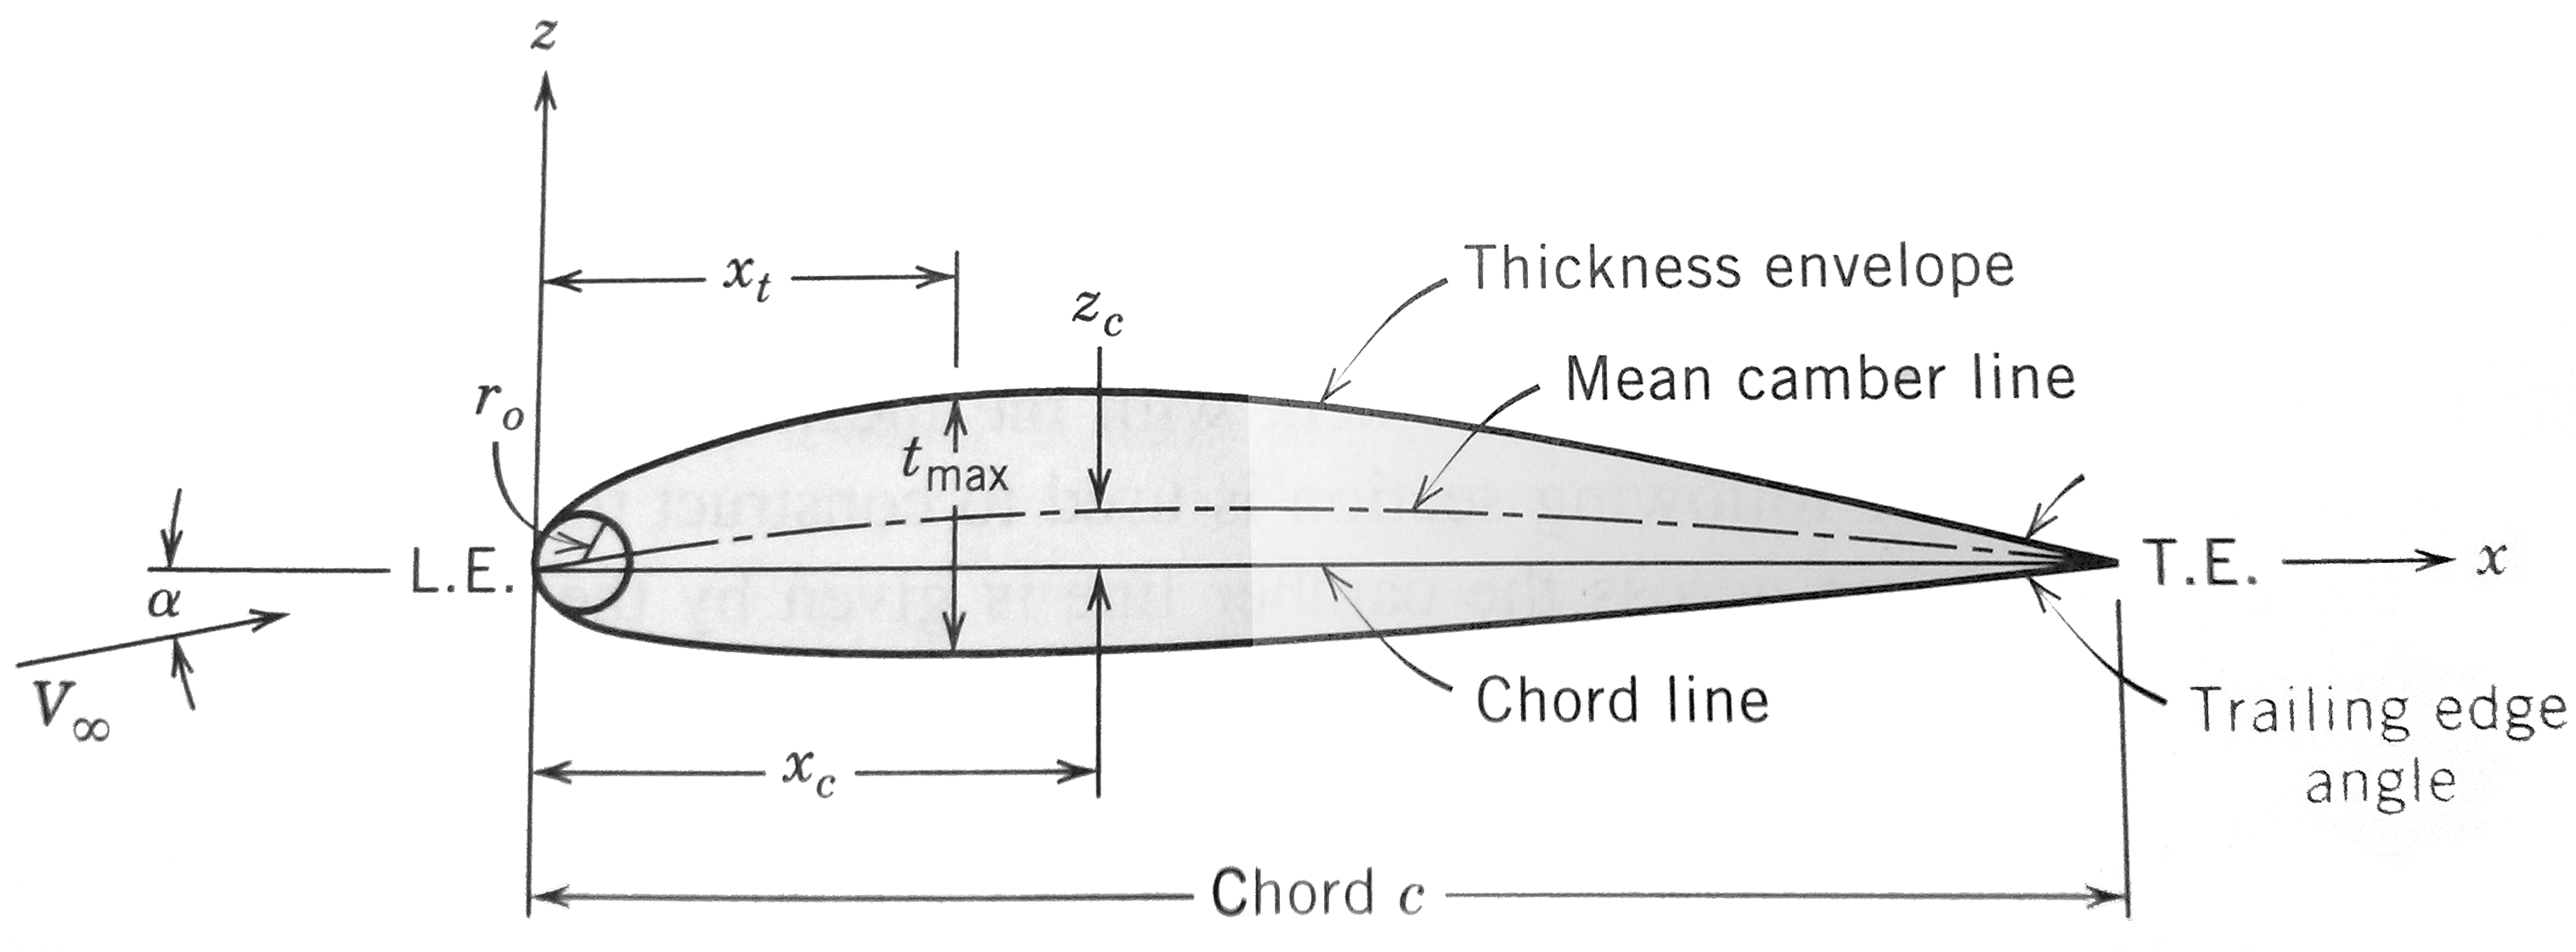
\includegraphics[width=\imagewidth]{images/background/airfoil.png}
    \caption{A depiction of the geometric properties of airfoil. The image was obtained from~\cite{kuethe1986foundations}.}
    \label{fig:airfoil-geometry}
\end{figure}

\section{Chapter summary}
In this chapter we gave a basic description of a mesh as a mathematical model. In addition we defined the concept of the mesh a data structure and how it is used in computation. Finally, we explained the significance of the airfoil in order to have a framing context for our running example.

\chapter{Related works}
We present a selection of prior works which touch upon the area of mesh structure, or are related to it in appealing ways.
% \section{Structure is beneficial}



% - How do quad meshes with subregions of structure come about
% - Are they seen often


\section{Structure detection and extraction}


Of all the works discussed in this chapter, \cite{tautges2004moab}~by Tautges is the most similar. The paper discusses the merits of structured meshes in great depth. It also defines the concept of disparate structured regions in a mesh, and discusses strategies for fusing them into a hierarchy of structures. A structure construction algorithm is also discussed very briefly.


% Fast Neighborhood Search on Polygonal Meshes
% http://www.inf.ethz.ch/personal/dpanozzo/papers/EGIT11-RocDeGPanPup.pdf
% Dude et al tackle the specific problem of neighborhood search by defining a spatial index, a hierarchy of clusters of vertices. Their method yields an approximation, ours is exact, with the mesh model left completely unaltered. However, we can learn a few things.

% The problem of indirections and its derivatives (non-contiguous memory access and its impact on cache hierarchy) is cited/highlighted as a key motivation in basing their mesh data structure on a geometric model, i.e. the spatial index. We undertake the opposite approach, viewing geometric data as mere associative data attached to a topological mesh model.

Adapting the mesh model to use a structured representation for the benefit of the relevant application domain is common practice.
Rocca et al.~\cite{rocca2011fast} address the particular problem of neighbourhood search: finding the set of vertices within a certain distance from a given vertex. They define a spatial index, a hierarchy of vertex clusters, that yields good approximations to neighbourhood search queries.

The problem of memory access indirections, associated with representing the mesh topology, is cited as a key motivation for basing their mesh data structure (the aforementioned spatial index) on a geometric model which does not require storing topological information. This is in sharp contrast to our approach of transforming the mesh topology representation, and treating the mesh geometry as arbitrary associated data.



% Motorcycle Graphs: Canonical Quad Mesh Partitioning
% http://www.ics.uci.edu/~goodrich/pubs/geomproc.pdf
% Whilst the motivations are different (mesh compression AND mesh isomorphism) the approach is similar:
% ``The simplest quadrilateral meshes are structured meshes, in which connections between quadrilaterals form a regular grid, but in complicated domains it may be necessary to use semi-regular meshes in which this structure is interrupted by a small number of extraordinary vertices that do not have degree four. We study how to partition a semi-regular mesh into a small number of structured submeshes.''


% ``To ensure that isomorphisms will always be found when they exist, our partition must be canonical: the same mesh must always generate the same partition. The partitioning algorithm we describe has this property.''
% We do not care about this property per se. There may be multiple optimal solutions for structure detection, for example.


% ``Additionally, these techniques may apply to areas beyond graphics such as scientific computation. Code for the finite element method can be greatly streamlined when applied to structured quadrilateral meshes. By partitioning unstructured meshes into structured submeshes, it should be possible to achieve similar speedups for semi-regular meshes.''

Eppstein et al.~\cite{eppstein2008motorcycle} describe a method for partitioning quadrilateral meshes into structured regions using the \emph{motorcycle graph} construction, whose inspiration came from the 1982 movie Tron. The algorithm works by placing particles on each \emph{extraordinary} vertex\footnote{\label{footnote:extraordinary-vertices} This is in contrast to an \emph{ordinary} vertex, which the authors define as ``a non-boundary vertex incident with four edges or a boundary vertex incident with at most three edges.''} in the mesh, and advancing them along edges until they collide. The enclosed regions formed by the paths represent structured regions.

Whilst the motivations are different, with the emphasis on applications in mesh compression and detecting mesh isomorphisms, the approach may be applicable to the scientific computation domain. Indeed, the authors state this explicitly:
\begin{quote}
These techniques may apply to areas beyond graphics such as scientific computation. Code for the finite element method can be greatly streamlined when applied to structured quadrilateral meshes. By partitioning unstructured meshes into structured sub-meshes, it should be possible to achieve similar speedups for semi-regular meshes.
\end{quote}

We note, however, that the method makes a stronger assumption about the mesh, in that its ``structure is interrupted by a \emph{small number} of extraordinary vertices that do not have degree four [emphasis added]''.


% There exist processes which explicitly attempt to produce semi-structured meshes, for example *BELOW* which uses domain specific knowledge about the source object to find long strips which can be made into quads.
% Automatic Decomposition and Efficient Semi-Structured Meshing of Complex Solids
% http://www.imr.sandia.gov/papers/imr20/Makem.pdf

Makem et al.~\cite{makem2012automatic} utilise properties of the modelled object to generate meshes with structured regions inherent. The presented method detects long thin shapes with simply defined geometry, such as length and curvature, and generates an appropriate structured region representing these shapes.



\section{Structure in parallel computation}
There is a plethora of work on mesh partitioning optimised for parallel computation. The techniques presented often frame their objectives around these maxims:
\begin{enumerate}
\item \label{item:maximize-locality} Maximize intra-partition locality, thereby minimizing cross-partition communication.
\item \label{item:minimize-size} Minimize partition size, subject to it being sufficiently large to counterbalance the communication overheads.
\item \label{item:maximize-number} The partitions should be balanced and plentiful in number, so as to utilise parallelism.
``A parallel computation is often only as efficient as the evenness with which its workload is distributed over the processors in a parallel machine.''
\end{enumerate}

Objective~\ref{item:maximize-locality} is certainly a desirable property for our structured regions, and is in fact precisely what we set forth to perform.
On the other hand, objectives~\ref{item:minimize-size} and \ref{item:maximize-number} are rather misaligned with our needs; indeed, a monolithic structured region spanning the entire mesh would represent the best case for us.

Thus some of the techniques which hold these conflicting\footnote{The objectives are in conflict in our context. These objectives are more suited for their parallel context, naturally} objectives may not be fully compatible, though they undoubtedly offer helpful inspiration.

With that said, extending our techniques towards parallel computation is an obvious future step, and such future works should likely re-evaluate their objectives in lieu of this.



% Guide to Partitioning Unstructured Meshes for Parallel Computing
% http://www.hector.ac.uk/cse/reports/unstructured_partitioning.pdf
% Very briefly describes several tools used for partitioning the mesh

A technical report by Ridley~\cite{ridley2010guide} briefly discusses methods for partitioning a mesh so as to maximize spatial data locality, in other words adjacent elements tend to have memory locations that are close. The partitioning is applied by recursively bisecting the mesh geometrically, such that geometrically close points tend to cluster together. The emphasis of the report is towards improving the performance of parallel computation, but the benefits of partitioning extend to serial processing as well.



% Hierarchical Partitioning Techniques for Structured Adaptive Mesh Refinement Applications
% http://www.s3lab.ece.ufl.edu/publication/jsuper.pdf
% Partitions mesh to exploit parallel computation whilst minimizing communication costs. This is done by \emph{exploiting} the hierarchical structure in a mesh. The approach focuses on partitioning for purposes of parallel computation, which involves a) minimizing communication costs; and b) maximizing locality within partitions. We focus solely on B.
% For **future works**, however, A would come into the picture as well, which would add an interesting dimension to the problem for further exploration.
% ``This scheme uses space filling curves (SFC), which are a class of locality preserving recursive mappings from n-dimensional to 1-dimensional space.''
% ALSO, note that this is *dynamic*. We can do that too in the future? :)

Li et al.~\cite{li2004hierarchical} follow a similar theme of parallel computation, although their methods deal with adaptive mesh refinement, where a mesh is dynamically refined in regions with a high calculation error. The refinement process induces a hierarchical structure, which the presented partitioning algorithms aim to exploit.



% Hierarchical hybrid grids: data structures and core algorithms for multigrid
% http://onlinelibrary.wiley.com/store/10.1002/nla.382/asset/382_ftp.pdf?v=1&t=hw5h84yv&s=bbe650e186f348823036d7426c24bd554ea00c1b

Bergen et al.~\cite{bergen2004hierarchical} employ structure-aware mesh refinement techniques, which construct a hierarchy of structured regions with each iterative refinement to the mesh. It is suggested that different element types, such as edges and faces, refined and stored separately, such that their distinct structuredness can be represented.

Since we use a simple structure representation, we make use of augmented structured regions, with different elements' structured region represented in a hierarchy.



% Stencils and Problem Partitionings: Their Influence on the Performance of Multiple Processor Systems
% http://ieeexplore.ieee.org/ielx5/12/35266/01676980.pdf?tp=&arnumber=1676980&isnumber=35266
% Partitioning a mesh based on its memory-access stencil. Again this is parallel oriented. Could be useful in defining the shape of the map access!

Reed et al.~\cite{reed1987stencils} focus on obtaining partitions best-suited to the \emph{stencil structure} associated with a particular computation, that is its neighbour-access pattern. They derive partition shapes for some common stencil structures, optimised to minimise inter-partition communication costs.

Tang et al.~\cite{tang2011pochoir} present a full-fledged \emph{Pochoir Stencil Compiler}. It specifies a domain-specific language that allows users to write a higher-level specification of a stencil computation embedded in C++ code. The compiler then automatically generates very efficient \emph{cache-oblivious}\footnote{The authors of~\cite{frigo1999cache} define a cache oblivious algorithm as that which ``[does not contain] parameters (set at either compile-time or runtime that can be tuned to optimize the cache complexity for the particular cache size and line length''} parallel loops that execute the stencil computation.

As discussed in subsection~\ref{subsec:given-kernel-function}, this is similar to our approach, where the structured regions are detected on the basis of relation-maps, such as cell-vertex or edge-cell maps.


% \url{https://www.cs.sfu.ca/~bgb2/personal/papers/nand11miccai.pdf}
% Bruv et al describe in [REF] the ``[construction of] curvature based features detectors to detect tube-like and sheet-like structures in DTI [diffusion tensor MRI]''. Differential equation-based methods are applied to characterize the ``'structured-ness'' of various components of the generated image, in terms of feature detection. Our focus is on detecting structuring in a precise manner, rather than a characteristic approach.

% FOR FUTURE WORKS: The differential equation approach may be an interesting tangent for future work, for instance applying it to geometric information to deduce areas of likely structure.


% \url{http://ieeexplore.ieee.org/ielx7/83/6490370/06476010.pdf?tp=&arnumber=6476010&isnumber=6490370}
% Again, approximate/heuristical image-based structure detection. The paper mentions low-level and high-level pattern detection.




% multiblock structured mesh partitioning algorithm
% http://www.geuz.org/pipermail/getdp/2000/000138.html
% Michael sends an email discussing stuff







% Structured Grid Computational Pattern
% (EITHER FROM:
%   Course: CS 4800, Fall 2010, School: Northeastern
%   OR
% Parallel Computing Laboratory - Berkley University)
% http://parlab.eecs.berkeley.edu/wiki/_media/patterns/structuredgrid-2.pdf
% http://view.eecs.berkeley.edu/wiki/Structured_Grids
% Good overview of the benefits of structured regions for computation.



\section{Exploiting structure}

% Approximate Topological Matching of Quadrilateral Meshes
% http://www.ics.uci.edu/~goodrich/pubs/approx-match.pdf
% Find matching subgraphs of two meshes, that is having the same topology.

% ``Our reason for using mesh compression instead is based on the desire to speed up the computation time in an algorithm that operates on quad meshes. Thus, our approach actually fits the spirit of other algorithms (e.g., see (33; 15; 14; 38)) that perform data compression so as to improve algorithmic performance.''
% Mentions reducing mesh representation for the purpose of improving computation time.


Eppstein et al.~\cite{eppstein2008approximate} explore the problem of approximate topological matching between given quadrilateral meshes, that is detecting isomorphisms between their submeshes. To this end they discuss various techniques based on \emph{particle shooting}\footnote{The motorcycle graph construction discussed in the paper by the same authors~\cite{eppstein2008motorcycle} is based on particle shooting.}: ``particles'' are placed on certain vertices (for example, extraordinary vertices\footref{footnote:extraordinary-vertices}) and are then ``'fired'' along the mesh using certain rules.

One such algorithm, termed ``The Greedy Algorithm'' by the authors, is shown to suffer from a problem when particles advancing along the same front can get out of sync. The problem is remarkably similar to our discussion about contiguous detection in subsection~\ref{subsec:contiguous-detection}.


% Opportunistic Data Structures with Applications
% http://people.unipmn.it/manzini/papers/focs00draft.pdf
% Discusses implicit data structures which minimize storage overheads due to auxiliary information


% \section{}


% Predictable memory access patterns versus *known* memory access pattern.



\section{Chapter summary}
In this chapter we discussed the similarities and differences between our work and that of a variety of published works centred at or homing around our scope of interest. We saw that the inefficiencies associated with unstructured representation are a common pain point, and we saw the great interest in the area of detecting structure to aid parallel computations. Some works presented exploited structure for other intriguing purposes.


\chapter{Diving into the problem}
\label{chap:diving-into-problem}
We begin by walking through an example mesh and examining the properties of the structure found within.

\section{A basic definition of structure}
What we would like is a form of structure which is
\begin{enumerate*}[label=\alph*)]
\item representable as a data structure, and \item efficient in terms of performance.
\end{enumerate*}

Given our semantic knowledge about the mesh model we can ascertain some facts about relation-maps:
\begin{itemize}
\item They are sparse: element arity is very small compared to the number of elements, and is in fact unrelated to it.
\item They have a high clustering coefficient: Relationships tend to be localized, forming tightly connected clusters.
% TODO REFERENCE TO CLUSTERING COEFFICIENTS
\end{itemize}

These properties arise as a consequence of meshes modelling real-world phenomena that exist in a Cartesian space.
On this basis, we consider a spatial embodiment of element relationships, organising the elements in a discrete space such that the uniform relationship is apparent.

Bear in mind that this approach carries no relation to any geometric data associated with elements, such as the coordinates of vertices. To make this distinction clear, as well as to emphasize its discrete nature, we address this Cartesian-like space by rows and columns rather than x and y coordinates.

\subsection{Example: Naca0012 mesh}
Figure~\ref{fig:naca12-plain} shows a small extract from the NACA0012 mesh\footnote{Thanks to Dr. Peter Vincent, George Ntemos and Harry Davis}, showing the cross section of an airfoil mesh and its interaction with surrounding fluid. The mesh is discretization into quadrilateral cells over which computations are performed.

\newcommand{\drawnaca}[4]{
	\begin{figure}
	\includesvg[svgpath=#1]{#2}
	\caption{#3}
	\label{#4}
	\end{figure}
}
\drawnaca{images/defining-structure/}{naca0012-plain}{Extract of the NACA0012 mesh.}{fig:naca12-plain}

The vertices in the highlighted region of figure~\ref{fig:naca12-vertices} seem like good candidates for a \emph{``structured region''}, forming a two-dimensional lattice in a discrete Cartesian space. This \emph{``structured region''} has the properties outlined below.

\drawnaca{images/defining-structure/}{naca0012-node-structure}{Highlighted vertices which exhibit a form of \emph{``structured region''}.}{fig:naca12-vertices}

\subsection{Desired properties of a structured region}
\label{sec:structured-region-properties}
\begin{enumerate}
\item All vertices have a uniform arity of four.
\item Every vertex has a consistent discrete direction (for example the cardinal directions: north east, south, west) with respect to the other vertices. In other words, the direction is transitive: if vertex $a$ is above vertex $b$, and vertex $b$ is above vertex $c$, then vertex $a$ is above vertex $c$. For a non-example see figure~\ref{fig:non-consistent-direction}.
\end{enumerate}

\begin{figure}
\includesvg[width=\imagewidth, svgpath=images/defining-structure/]{non-consistent-direction}
\caption{An example of inconsistent direction. We can traverse cells in \emph{``one direction''} by following the edge parallel to the one we entered from. If we start from $A$ and traverse the cells in one direction (the blue path) we reach $Z$. If we start from $A$ and traverse the cells in an orthogonal direction (the red path) to the first path, we also reach $Z$! Is $Z$ then \emph{``above''} $A$ or \emph{``to the side of it''}?}
\label{fig:non-consistent-direction}
\end{figure}


%% TODO Maybe not introduce data structure yet????
We can propagate this inherent structure from the mesh model to the underlying data structure, representing this two-dimensional lattice using a two-dimensional array. Vertices may be assigned Cartesian coordinates, but in spirit of the space's discreteness we shall use rows and columns instead. See figure~\ref{fig:naca12-structure-grid}.\label{sentence:2d-array}

\drawnaca{images/defining-structure/}{naca0012-node-grid}{The overlaid grid shows the lattice structure more clearly.}{fig:naca12-structure-grid}


\newcommand{\strV}{V_{str}}
\newcommand{\adjstrV}{V_{adjstr}}
\newcommand{\AdjVVstr}{Adj_{\adjstrV\strV}}

Let us call $\VertexSet$ the set of all vertices, and $\strV \subseteq \VertexSet$ the set of vertices in the \emph{``structured region''}.

\subsection{Representing the vertex-vertex adjacency}

Now consider the vertex-vertex adjacency relation $\AdjVV: \VertexSet \mapsto \VertexSet$ in context of the \emph{``structured region''} $\strV$. We can directly locate a particular neighbour of any vertex, for example its north neighbour, so long as that neighbour is also within the structured region. This restricts the set of vertices with fully-accessible neighbours to those which are not on the borders or the fringe of the \emph{``structured region''}. This is the subset of vertices $\adjstrV \subseteq \strV$ which are structured \emph{with respect to} $\AdjVV$. This induces a new relation which operates purely within the structured region:
$$\AdjVVstr: \adjstrV \mapsto \strV$$

Figures~\ref{fig:naca12-structured-highlighted} and~\ref{fig:structure-as-graph} illustrate these two sets.
\drawnaca{images/defining-structure/}{naca0012-node-neighbours}{The interior structured vertices (those not on the fringe) are highlighted in dark blue.}{fig:naca12-structured-highlighted}


\begin{figure}
% Draw structured node region
\begin{tikzpicture}[scale=0.7]
	\newcommand{\stylewithfill}[1]{\tikzstyle{every node}=[draw, shape=circle, minimum size=0.8cm, fill=#1];}
	\stylewithfill{none}

	% ROW 0
	\drawgrid{rows=1, cols=3, rowoffset=0, coloffset=4, labeler=\plainlabelnode, labelerA=0, labelerB=2,
		southborder=structured}

	% ROW 1
	\drawgrid{rows=1, cols=2, rowoffset=-2, coloffset=0, labeler=\plainlabelnode, labelerA=1, labelerB=0,
		eastborder=structured}

	{
	\stylewithfill{neighbourstructurecolor}
	\drawgrid{rows=1, cols=2, rowoffset=-2, coloffset=4, labeler=\plainlabelnode, labelerA=1, labelerB=2,
		northborder=structured, southborder=structured, westborder=structured, eastborder=structured}
	}

	\drawgrid{rows=1, cols=1, rowoffset=-2, coloffset=8, labeler=\plainlabelnode, labelerA=1, labelerB=4,
		northborder=structured, southborder=structured, westborder=structured}


	\drawgrid{rows=1, cols=1, rowoffset=-2, coloffset=12, labeler=\plainlabelnode, labelerA=1, labelerB=6,
		southborder=structured, eastborder=structured}

	\drawgrid{rows=1, cols=1, rowoffset=-2, coloffset=14, labeler=\plainlabelnode, labelerA=1, labelerB=7,
		westborder=structured}

	% ROW 2
	\drawgrid{rows=1, cols=1, rowoffset=-4, coloffset=4, labeler=\plainlabelnode, labelerA=2, labelerB=2,
		northborder=structured, southborder=structured, eastborder=structured}

	{
	\stylewithfill{neighbourstructurecolor}
	\drawgrid{rows=1, cols=2, rowoffset=-4, coloffset=6, labeler=\plainlabelnode, labelerA=2, labelerB=3,
		northborder=structured, southborder=structured, eastborder=structured, westborder=structured}
	}

	\drawgrid{rows=1, cols=1, rowoffset=-4, coloffset=10, labeler=\plainlabelnode, labelerA=2, labelerB=5,
		southborder=structured, westborder=structured, eastborder=structured}

	\drawgrid{rows=1, cols=1, rowoffset=-4, coloffset=12, labeler=\plainlabelnode, labelerA=2, labelerB=6,
		northborder=structured, westborder=structured}

	% ROW 3
	\drawgrid{rows=1, cols=1, rowoffset=-6, coloffset=4, labeler=\plainlabelnode, labelerA=3, labelerB=2,
		northborder=structured, southborder=structured, eastborder=structured}

	{
	\stylewithfill{neighbourstructurecolor}
	\drawgrid{rows=1, cols=2, rowoffset=-6, coloffset=6, labeler=\plainlabelnode, labelerA=3, labelerB=3,
		northborder=structured, southborder=structured, eastborder=structured, westborder=structured}
	}

	\drawgrid{rows=1, cols=1, rowoffset=-6, coloffset=10, labeler=\plainlabelnode, labelerA=3, labelerB=5,
		northborder=structured, westborder=structured}

	% ROW 4
	\drawgrid{rows=1, cols=1, rowoffset=-8, coloffset=2, labeler=\plainlabelnode, labelerA=4, labelerB=1, eastborder=structured}

	{
	\stylewithfill{neighbourstructurecolor}
	\drawgrid{rows=1, cols=2, rowoffset=-8, coloffset=4, labeler=\plainlabelnode, labelerA=4, labelerB=2,
		northborder=structured, southborder=structured, eastborder=structured, westborder=structured}
	}

	\drawgrid{rows=1, cols=1, rowoffset=-8, coloffset=8, labeler=\plainlabelnode, labelerA=4, labelerB=4,
		northborder=structured, westborder=structured}

	% ROW 5
	\drawgrid{rows=1, cols=2, rowoffset=-10, coloffset=4, labeler=\plainlabelnode, labelerA=5, labelerB=2,
		northborder=structured}
\end{tikzpicture}
\caption{The vertices in figure~\ref{fig:naca12-structured-highlighted} represented as a graph.}
\label{fig:structure-as-graph}
\end{figure}

The key insight we make is that for structured regions in a mesh we need not represent set relationship maps explicitly; the uniformity of set relations allows us to deduce the relationships. We can encode the relation $\AdjVVstr$ very simply. Given a vertex $n_{r,c} \in \adjstrV$, located at row $r$ and column $c$, its four vertex neighbours are $n_{r,c-1}$, $n_{r,c+1}$, $n_{r-1,c}$, and $n_{r+1,c}$. This is illustrated in figure~\ref{fig:single-vertex-neighbours}.



\begin{figure}
% Draw structured node region
\begin{tikzpicture}[scale=1]
	\newcommand{\stylewithfill}[1]{\tikzstyle{every node}=[draw, shape=circle, minimum size=1.3cm, fill=#1];}
	\stylewithfill{none}

	% ROW 0
	\drawgrid{rows=1, cols=1, rowoffset=0, coloffset=2,
		labeler=\varlabelnode, labelerA=-1, labelerB=0, labelerC=r, labelerD=c,
		southborder=structured}

	% ROW 1
	\drawgrid{rows=1, cols=1, rowoffset=-2, coloffset=0,
		labeler=\varlabelnode, labelerA=0, labelerB=-1, labelerC=r, labelerD=c,
		eastborder=structured}

	{
		\stylewithfill{neighbourstructurecolor}
		\drawgrid{rows=1, cols=1, rowoffset=-2, coloffset=2,
			labeler=\varlabelnode, labelerA=0, labelerB=0, labelerC=r, labelerD=c,
			eastborder=structured, westborder=structured, northborder=structured, southborder=structured}
	}

	\drawgrid{rows=1, cols=1, rowoffset=-2, coloffset=4,
		labeler=\varlabelnode, labelerA=0, labelerB=1, labelerC=r, labelerD=c,
		westborder=structured}

	% ROW 2
	\drawgrid{rows=1, cols=1, rowoffset=-4, coloffset=2,
		labeler=\varlabelnode, labelerA=1, labelerB=0, labelerC=r, labelerD=c,
		northborder=structured}

\end{tikzpicture}
\caption{The neighbours of a structured vertex.}
\label{fig:single-vertex-neighbours}
\end{figure}


\section{Mesh structure as a data structure}
The choice of data structure to represent the structured region is a key one, touching on various aspects:
\begin{itemize}
\item Scope of structure representation: what level of structure can be represented.
\item Implementation complexity of structure detection: how complex a detection algorithm is required.
\item Runtime performance of structure detection: the time and space complexity of the detection algorithm.
\item Storage requirements for detected structure: the storage requirements for the detected structure.
\item Runtime performance of computation over the structured region.
\end{itemize}

We analyse several possible data structure representations.

\subsection{Structure bit-mask}
\label{subsec:structure-bitmap}

\newcommand{\drawbitmap}[2]{
	% trim left bottom right top
	\includesvg[svgpath=#1]{#2}
}

Represent the bounding box around the structured region as a two-dimensional bit-mask, with each bit representing a vertex position in the superimposed grid. An \emph{on} bit indicates that the corresponding vertex is part of the structured region, an \emph{off} bit otherwise.

A bit-mask can represent \emph{any} structured region which adheres to the properties listed in section~\ref{sec:structured-region-properties}. They are very flexible, capable of representing complex formations as well as handling small anomalies in structure.

Let us define the \emph{efficiency} $\epsilon$ of a bit-mask as the percentage of its bits which are \emph{on}, as the \emph{off} bits represent wasted vertices. Bit-masks with high $\epsilon$ are favourable for several reasons:
\begin{itemize}
\item \emph{Off} bits increase the storage space of the structured region, up to $O(\card{\VertexSet})$ in the worst case, as opposed to $O(\card{\Structured})$.
\item \emph{Off} bits similarly worsen the runtime performance, again up to $O(\card{\VertexSet})$ due to wasted execution.
\end{itemize}

Figure~\ref{fig:example-bitmask} shows an example of a good bit-mask candidate.

\begin{figure}
\pgfplotstableread{
	1 1 1 1 1 1
	1 2 2 1 1 1
	1 1 2 1 1 2
	1 1 1 1 1 1
	1 1 1 1 1 2
	2 1 1 1 1 1
}{\bitmapmatrix}
\drawmatrix[cell wd=0.8, cell ht=0.8]{\bitmapmatrix}
\caption{An example of a structured region which can be bit-mask defined. The dotted regions indicate unstructured cells. The blue cells are structured cells. Its efficiency $\epsilon$ is $\frac{30}{36} \approx 83\%$.}
\label{fig:example-bitmask}
\end{figure}

A detection algorithm would likely be implemented using a variant of a general graph search algorithm such as breadth-first search or depth-first search. Further consolidation work may be needed to compact disconnected structured components in order to maximize $\epsilon$. The potential benefits of compaction are illustrated in figure~\ref{fig:disjoint-matrix}.

\begin{figure}
\pgfplotstableread{
	2 2 2 2 2 1
	1 2 2 2 2 1
	1 1 2 2 2 2
	2 1 2 2 2 2
	2 1 2 1 2 2
	2 1 1 1 2 2
}{\disjointAmatrix}
\pgfplotstableread{
	1 2 2 1
	1 1 2 1
	2 1 2 2
	2 1 2 1
	2 1 1 1
}{\disjointBmatrix}

\sidebyside
{
\drawmatrix[cell wd=0.8, cell ht=0.8]{\disjointAmatrix}
\caption{Originally detected structured components.}
\label{subfig:original-components}
}
{
\drawmatrix[cell wd=0.8, cell ht=0.8]{\disjointBmatrix}
\caption{Compacted structured components.}
\label{subfig:compacted-components}
}
\caption{A demonstration of the benefits of disconnect structured components compaction. The detected structured cell components in~\ref{subfig:original-components} are unnecessarily sparse and occupy more space than necessary. After compaction in~\ref{subfig:compacted-components} the space is used is reduced by over 40\%.}
\label{fig:disjoint-matrix}
\end{figure}


\subsection{Row-specific boundaries}

Represent the structured region as a sequence of consecutive fixed-length rows, permitting vertices outside the structured region to cluster at the beginning and ends of each row. A structured region is then represented by the row-length, as well as individual begin and end offsets for each row. This is exemplified in figure~\ref{fig:row-specific}.

\begin{figure}
\pgfplotstableread{
	0 2 1 1 1 1
	2 2 1 1 1 2
	1 1 1 1 2 0
	2 1 1 1 1 1
	1 1 1 1 1 1
	2 2 1 1 2 2
}{\bitmapmatrix}
\drawmatrix[cell wd=0.8, cell ht=0.8]{\bitmapmatrix}
\caption{An example of a structured region which can be represented using row-specific boundaries. Note the white cells, which represent unused structured regions near the boundaries.}
\label{fig:row-specific}
\end{figure}

Storing row-specific boundaries reduces the storage requirement by the order of row-length times.
No executions are wasted as the loop iterations are constrained to vertices in the structured region.
A detection algorithm can be implemented as a simple row-by-row traversal in linear time and space.


On the downside, this scheme trades some of the flexibility offered by the bit-mask representation, in particularly anomalies in structure which do not occur at the boundaries.


\subsection{Full rectangle}

Represent the structured region as a rectangle of given length and width, with all elements corresponding strictly to vertices within the structured region. The structured region is thus simply represented by the length and the width: the number of rows and the number of columns. Figure~\ref{fig:rectangle} shows an example of a rectangle-representable structured region.

The storage requirement is now constant with respect to the size of the structured region.
Loop iterations are fixed for each region, enabling further optimisation opportunities.
A detection algorithm, as above, can be implemented as a simple row-by-row traversal.

On the downside, the scope of structure representable is limited, being only capable of representing rectangles proper. Nonetheless, we stick with detecting rectangular structured regions for the remainder of this work as it seems to be the most promising choice.

\begin{figure}
\pgfplotstableread{
	0 2 2 0 2 0
	2 2 1 1 2 2
	2 0 1 1 2 2
	2 2 1 1 0 0
	0 2 1 1 2 2
	2 2 1 1 2 2
}{\bitmapmatrix}
\drawmatrix[cell wd=0.8, cell ht=0.8]{\bitmapmatrix}
\caption{An example of a rectangular structured region. Note the abundance of unused structured cells.}
\label{fig:rectangle}
\end{figure}

\section{Chapter summary}
In this chapter we derived intuitive definitions structure in a mesh in light of an excerpt from an airfoil mesh. We also discussed different representations in which they can be manifested, and the advantages and disadvantages of each.

\chapter{Rectangle growth strategy}
This chapter covers the detection of rectangular structured regions.

An abstract discussion of various properties of algorithms is presented, and the desirable traits brought forth by each.
Then, a selection of concrete algorithms are described, and their merits and weaknesses examined.


\section{Key concepts}
An \emph{absolute structured position} refers to the position of a structured element with respect to the boundaries of its structured region.
A \emph{relative structured position} refers to the position of a structured element with respect to other structured elements within its structured region. Figure~\ref{fig:structured-position} shows this through an example.


%% Relative vs absolute
\begin{figure}
\newcommand{\nodesize}{1.2}
\newcommand{\rows}{4}
\newcommand{\cols}{4}
\newcommand{\rowsize}{\rows*\nodesize}
\newcommand{\colsize}{\cols*\nodesize+2*0.1}

% Node at position r, c, label
\newcommand{\nodeat}[3]{
	\pgfmathsetmacro{\lerow}{ (\rows - #1) * \nodesize - (\nodesize / 2) - 0.1}
	\pgfmathsetmacro{\lecol}{ (#2 * \nodesize) + (\nodesize / 2) + 0.1}
	\node at (\lecol, \lerow) {#3}
}

\sidebyside
{
	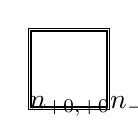
\begin{tikzpicture}
		\tikzstyle{every node}=[draw, shape=rectangle, minimum size=\nodesize cm, font=\small];
		\draw[double] (0,0) rectangle (\colsize,\rowsize);
		\nodeat{2}{1} {$n_{+0,+0}$};
		\nodeat{1}{1} {$n_{-1,+0}$};
		\nodeat{2}{2} {$n_{+0,+1}$};
	\end{tikzpicture}
	\caption{Relative structured position\label{fig:relative-structured-position}}
}
{
	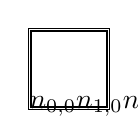
\begin{tikzpicture}
		\tikzstyle{every node}=[draw, shape=rectangle, minimum size=\nodesize cm, font=\small];
		\draw[double] (0,0) rectangle (\colsize,\rowsize);
		\nodeat{0}{0} {$n_{0,0}$};
		\nodeat{1}{0} {$n_{1,0}$};
		\nodeat{0}{1} {$n_{0,1}$};
	\end{tikzpicture}
	\caption{Absolute structured position\label{fig:absolute-structured-position}}
}
\caption{Depiction of \emph{relative} structured position versus \emph{absolute} structured position. The row and column counts are increasing down and to the right, respectively. The borders indicate structured regions, whose origin resides in the top-left corner.\label{fig:structured-position}}
\end{figure}



\section{Properties of detection algorithm}

\subsection{Eager detection}
An eager (or greedy) detection algorithm will include every structured element if finds immediately, regardless of the long term consequences. While this strategy may lead to suboptimal results, it avoids backtracking the structure detection which may be prohibitively costly. Figure~\ref{fig:eager-detection} depicts the sub-optimality of eager detection in contrast with non-eager detection.


\begin{figure}
\pgfplotstableread{
	2 2 2 2 2 2 0
	2 2 1 2 2 0 0
	0 0 1 0 0 0 0
	0 0 1 0 0 0 0
}{\eagermatrix}
\pgfplotstableread{
	2 2 2 2 2 2 0
	2 2 0 2 2 0 0
	1 1 1 1 1 1 1
	1 1 1 1 1 1 1
}{\noneagermatrix}

\sidebyside
{
	\drawmatrix[cell wd=0.6, cell ht=0.6]{\eagermatrix}
	\caption{Eager detection may greedily add the northern cell, yielding a suboptimal structured region.}
}
{
	\drawmatrix[cell wd=0.6, cell ht=0.6]{\noneagermatrix}
	\caption{A non-eager algorithm could instead decide to ignore the northern cell, yielding a larger structured region.}
}
\caption{Eager versus non-eager detection. Black cells and white cells denote unstructured and structured elements, respectively. Red cells denote structured elements detected as forming a rectangular structured region.\label{fig:eager-detection}}
\end{figure}



\subsection{Contiguous detection}
\label{subsec:contiguous-detection}
An algorithm which exhibits continuous detection always adds a structured element which is contiguous to the structured region thus far. The implication is that the relative structured position is always known. This greatly simplifies detection, as all adjacent structured elements are known at any point in time, and structured elements need not be repositioned in the structured region. Figure~\ref{fig:contiguous-detection} contrasts contiguous detection with non-contiguous detection.

In the case of non-contiguous detection, any non-contiguous blobs need to be consolidated. These blobs may be one of three cases:
\begin{enumerate}
\item Disjoint
These may simply be taken as two separate structured regions.

\item Compatible
The blobs can be merged in a lossless manner to form a single structured region.

\item Incompatible
The blobs cannot be merged without loss of structure due to inconsistencies between the blobs. It is then necessary to discard some structured elements.
\end{enumerate}

Examples of the three cases are shown in figure~\ref{fig:non-contiguous-detection}.


% Contiguous versus non-contiguous
\begin{figure}
\pgfplotstableread{
	0 1 1 1 0 0 0 0 0
	0 1 1 1 1 0 0 0 0
	0 1 1 1 0 0 0 0 0
	0 0 1 0 0 0 0 0 0
	0 0 0 0 0 0 0 0 0
}{\contiguousmatrix}
\pgfplotstableread{
	0 1 1 1 0 0 0 0 0
	0 1 1 1 1 0 0 1 0
	0 1 1 1 0 0 1 1 0
	0 0 1 0 0 0 0 0 0
	0 0 0 0 0 0 0 0 0
}{\noncontiguousmatrix}

\sidebyside
{
	\drawmatrix[cell wd=0.6, cell ht=0.6]{\contiguousmatrix}
	\caption{Contiguous detection always adds cells adjacent to the structured region detected thus far.}
}
{
	\drawmatrix[cell wd=0.6, cell ht=0.6]{\noncontiguousmatrix}
	\caption{Non-contiguous detection may add cells which do not border the structured region detected thus far.}
}
\caption{Contiguous detection versus non-contiguous detection algorithms. White cells denote structured elements which have not been added to the structured region. Red cells denote structured elements detected thus far.\label{fig:contiguous-detection}}
\end{figure}

% Types of non-contiguous
\begin{figure}
\sidebysidethreevertical
{
	\includesvg[svgpath=images/detection-algorithms/,width=60mm]{disjoint-blobs}
	\caption{Disjoint blobs of structured elements.}
}
{
	\includesvg[svgpath=images/detection-algorithms/,width=60mm]{compatible-blobs}
	\caption{Compatible blobs of structured elements.}
}
{
	\includesvg[svgpath=images/detection-algorithms/,width=60mm]{incompatible-blobs}
	\caption{Incompatible blobs of structured elements. The two dashed cells are not adjacent in the mesh, but if added as structured element they would have adjacent positions in the structured region.}
}
\caption{Cases that may arise with non-contiguous detection.\label{fig:non-contiguous-detection}}
\end{figure}


\subsection{Post processing requirements}
Different algorithms will require different levels of post-processing in order to yield a rectangular structured region. Some may require a simple operation, such as trimming incomplete rows, while others may require more complex operations to achieve this goal.


\subsection{Detection traversal patterns}
The order in which structured elements are detected in a structured region is important; it imposes some constraints on the data structure representing it. Given the dimensions of the structured region, and knowledge of the absolute structured positions of elements as they are discovered, a simple 2D array allocation would suffice. Any detection order, as is convenient, may be used in this case. However, neither of those facts are known a priori in general.

Various detection traversals orders and their merits are discussed below. Figure~\ref{fig:detection-traversal-patterns} outlines some examples.

\subsubsection{Single-row append-only}
\label{append-detection}
The structured region is grown in a constant direction, for example a single row of structured elements, appended to consecutively. This can be implemented efficiently using either a singly-linked list or a dynamic array with amortized constant time append operation.

\subsubsection{Single-row append/prepend}
\label{append-prepend-detection}
The structured region is grown in either of two directions, for example a single row of structured elements, appended and prepended to. This can be implemented efficiently using a double-ended queue with amortized constant time append and prepend operations.

\subsubsection{Row-oriented detection}
The structured region is represented as a group of rows, with the elements in individual rows grown using one of the above methods. The order in which the rows themselves are grown may also be utilize the same methods, with a nested data structure being a suitable implementation. For example, if rows are detected in an append-only fashion, and the individual elements are detected using append and prepend operations, then a suitable data structure would be a singly-linked list of double-ended queues.

\subsubsection{Indeterminate order detection}
The structured region is grown in a non-linear order: grown elements may not always be contiguous to the structured region thus far. If the growth is indeed non-contiguous, the relative structured positions are \emph{not} always known, and structured elements may need to be repositioned. A possible implementation would be a jagged 2D array, that is an array of arrays, which is expanded as needed. A flat-array-based 2D array would (in the worst case) require reallocating all elements upon expansion, as opposed to reallocating a single row in the case of a jagged 2D array.


% Detection traversal patterns
\begin{figure}
\sidebysidefour
{
	\includesvg[svgpath=images/detection-algorithms/,height=10mm]{append-detection}
	\caption{Single-row append detection.}
}
{
	\includesvg[svgpath=images/detection-algorithms/,height=10mm]{append-prepend-detection}
	\caption{Single-row append/prepend detection.}
}
{
	\includesvg[svgpath=images/detection-algorithms/,height=34mm]{row-oriented}
	\caption{Row-oriented detection, with rows detected in an append-only fashion, and elements within rows in an append/prepend fashion.}
}
{
	\includesvg[svgpath=images/detection-algorithms/,height=51mm]{indeterminate-detection}
	\caption{Indeterminate order detection. Note that some possible regions of expansions are not adjacent to the presently detected structured region.}
}
\caption{Examples of detection traversal patterns. The red blocks represent presently detected structured regions. The dashed pink blocks represent possible regions for expansion.\label{fig:detection-traversal-patterns}}
\end{figure}




Consider contiguity in a figure!!!!

---------------------
                    |
                    |
          A         |
        -------------
     B  | C |
        |----
        |
---------

If the the region were to be grown to include include element C, it must be the case that C is adjacent to both A and B, but is not adjacent to any other structured element thus far. Since the structure is always contiguous, we know at every point whether any two structured elements ought to be adjacent.


\section{Detection algorithms}

\subsection{Length-first search}

\begin{enumerate}
\item Starting from a seed vertex, grow a quad.

\item The quad is grown along one axis, both forwards and backwards, as far as possible, forming the length of the structured region. This is a per-row append/prepend traversal.
\item The row grown above is extended along the orthogonal axis, both forwards and backwards, as far as possible. Each expanded row must have the length of the initial row exactly, forming the width of the structure region. This is a row-oriented append/prepend traversal.
\end{enumerate}

The detection is clearly contiguous, with all structured element insertions running in amortized constant time. Only a constant amount of extra storage is required.

The algorithm is also an eager one, deciding the length of the structured region based on the first row it detects. This simple approach, however, can result in suboptimal detection.



\subsection{Descending-staircase search}
\begin{enumerate}
\item Follow the same steps as in length-first search, with one exception: in step~\ref{step:row-expansion}, each expanded row may have a length which is at most the length of its predecessor.
\item Find the rectangle with the maximum area, using an algorithm such as XXXXXX.
\end{enumerate}



Two types of techniques exist: seed-based, and global based. A seed-based technique starts with a seed, and grows from there. A global-based technique starts with all the orthogonal axis
% %TODO discuss random seed strategy

\chapter{Structure Extraction}
\label{chap:detect-quad-grid}
Taking forth our length-first search algorithm, we expand fill in the details glossed over by our earlier discussion, delineating it into a formal algorithmic specification.

% Initial vertex
\newcommand{\vinit}{v_{init}}

\newcommand{\Quad}[4]{\begin{bmatrix} #1 & #2 \\ #3 & #4 \end{bmatrix}}

% Initial quad
\newcommand{\Qinit}{\Quad{n_{1,1}} {n_{1,2}} {n_{2,1}} {n_{2,2}} }

% Initial quad mirrored about y-axis
\newcommand{\Qinitmirror}{\Quad {n_{1,2}} {n_{1,1}} {n_{2,2}} {n_{2,1}}}



\section{Inputs}
\begin{enumerate}
\item A non-reflexive and symmetric vertex-vertex adjacency relation:
$$ \AdjVV: \VertexSet \mapsto \powerset{\VertexSet} $$

\item A set of visited vertices
$$ \Visited \subseteq \VertexSet $$

\item An unvisited start vertex
$$ \vinit \in \VertexSet \setminus \Visited $$
\end{enumerate}


\section{Outputs}
\begin{enumerate}
\item A structured set of vertices $\Structured \subseteq \VertexSet \setminus \Visited $ forming the extracted structured region.
The vertices $\Structured$ are structured on a 2-dimensional Cartesian lattice with $m$ rows and $n$ columns.
\end{enumerate}


%%%% PHASE 1

%% Phase 1 summary
\section{Phase 1: Grow a quad}
\label{sec:grow_a_quad}
Starting from the initial vertex $\vinit$, call it $n_{1,1}$, we would like to discover three other vertices $n_{1,2}$, $n_{2,1}$, and $n_{2,2}$ such that $\Qinit$ forms a valid quad in a structured quad region. They must satisfy the following constraints:

\begin{itemize}
\item Each of the four vertices must have exactly 4 neighbours.
\item Each of the following pairs of vertices are neighbours: $n_{1,1}$~and~$n_{1,2}$ ; $n_{1,2}$~and~$n_{2,2}$ ; $n_{2,2}$~and~$n_{2,1}$ ; $n_{2,1}$~and~$n_{1,1}$.
\item Each of the vertices must \emph{not} neighbour any vertex that has been visited thus far, apart from those vertices explicitly mentioned.
\end{itemize}

%% Phase 1 diagram

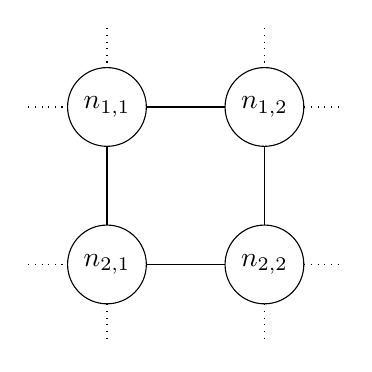
\begin{tikzpicture}[scale=1]
	% Default action for each node
	\tikzstyle{every node}=[draw, shape=circle, minimum size=1cm];

										\coordinate (northleft) at (0, 2);	\coordinate (northright) at (2, 2);
	\coordinate (westup) at (-1,1);		\node (r1c1) at (0,1) {$n_{1,1}$};	\node (r1c2) at (2,1) {$n_{1,2}$};	\coordinate (eastup) at (3,1);
	\coordinate (westdown) at (-1,-1);	\node (r2c1) at (0,-1) {$n_{2,1}$};	\node (r2c2) at (2,-1) {$n_{2,2}$};	\coordinate (eastdown) at (3,-1);
										\coordinate (southleft) at (0, -2);	\coordinate (southright) at (2, -2);

	% Horizontals
	\draw[outside] (westup) -- (r1c1);
	\draw (r1c1) -- (r1c2);
	\draw[outside] (r1c2) -- (eastup);

	\draw[outside] (westdown) -- (r2c1);
	\draw (r2c1) -- (r2c2);
	\draw[outside] (r2c2) -- (eastdown);

	% Verticals
	\draw[outside] (northleft) -- (r1c1);
	\draw (r1c1) -- (r2c1);
	\draw[outside] (r2c1) -- (southleft);

	\draw[outside] (northright) -- (r1c2);
	\draw (r1c2) -- (r2c2);
	\draw[outside] (r2c2) -- (southright);
\end{tikzpicture}

%% Phase 1 algorithm

\subsection{Algorithm}

\begin{enumerate}
\item If $\vinit$ does not have exactly 4 neighbours, that is $ \card{\AdjVV(\vinit)} \neq 4 $, return immediately with $\Structured = \varnothing$.
\item Let $ n_{1,1} = \vinit $, and let $ a, b, c \in \AdjVV(\vinit) $ be distinct vertex neighbours of $\vinit$. Consider vertices $a$ and $b$. If they do not both have exactly 4 neighbours, then they cannot form a part of a structured quad region. Return immediately with $\Structured = \varnothing$.

\item Otherwise, there are three cases:

	%%%% BEGIN THREE CASES
	\begin{enumerate}

	%% Straight line case
	\item $a$ and $b$ have exactly one neighbour in common, which must be $n_{1,1}$ by construction, expressed by:
	$$ \card{\AdjVV(a) \cap \AdjVV(b)} = 1$$
	$a, n_{1,1}, b $ are \emph{topologically} along a straight line of a structured grid, and hence cannot form a quad.
	We therefore consider $b$, $n_{1,1}$, and  $c$ instead as candidates, letting $n_{2,1} = b$ and $n_{1,2} = c$.
	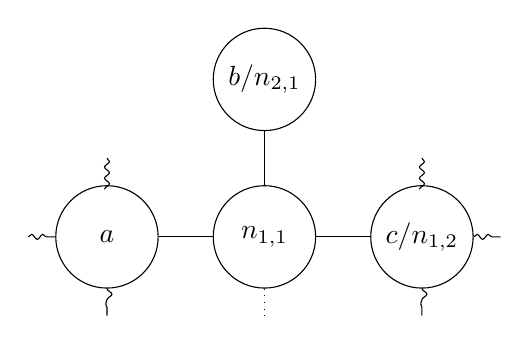
\begin{tikzpicture}
		% Default action for each node
		\tikzstyle{every node}=[draw, shape=circle, minimum size=1.3cm];

										\coordinate (northleft) at (-1,2);	\node (b) at (1,3) {$b / n_{2,1}$};	\coordinate (northright) at (3,2);
		\coordinate (west) at (-2,1);	\node (a) at (-1,1) {$a$};			\node (n11) at (1,1) {$n_{1,1}$};	\node (c) at (3,1) {$c / n_{1,2}$};	\coordinate (east) at (4,1);
										\coordinate (southleft) at (-1,0);	\coordinate (southmid) at (1,0);	\coordinate (southright) at (3,0);

		% Horizontals
		\draw[anywhere] (west) -- (a);
		\draw (a) -- (n11) -- (c);
		\draw[anywhere] (c) -- (east);

		% Verticals
		\draw[anywhere] (northleft) -- (a) -- (southleft);
		\draw (b) -- (n11);
		\draw[outside] (n11) -- (southmid);
		\draw[anywhere] (northright) -- (c) -- (southright);
	\end{tikzpicture}


	%% Angle case
	\item $a$ and $b$ have exactly two neighbours in common, one of which must be $n_{1,1}$ by construction, expressed by:
	$$ \card{\AdjVV(a) \cap \AdjVV(b)} = 2$$
	We continue with vertices $a$, $n_{1,1}$, and $b$ as candidates, letting $n_{2,1} = a$ and $n_{1,2} = b$.
	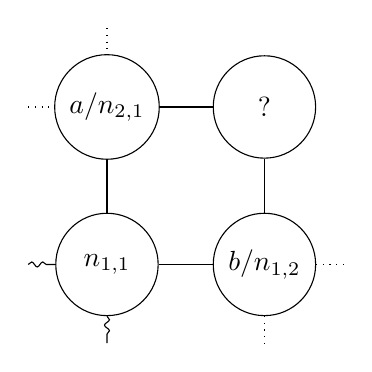
\begin{tikzpicture}
		% Default action for each node
		\tikzstyle{every node}=[draw, shape=circle, minimum size=1.3cm];

											\coordinate (northleft) at (-1,4);		\coordinate (northright) at (1,4);
		\coordinate (westup) at (-2,3);		\node (a) at (-1,3) {$a / n_{2,1}$};	\node (d) at (1,3) {$?$};			\coordinate (eastup) at (2,3);
		\coordinate (westdown) at (-2,1);	\node (n11) at (-1,1) {$n_{1,1}$};		\node (b) at (1,1) {$b / n_{1,2}$};	\coordinate (eastdown) at (2,1);
											\coordinate (southleft) at (-1,0);		\coordinate (southright) at (1,0);



		\draw[outside] (westup) -- (a);
		\draw (a) -- (d);
		% \draw (d) -- (eastup);

		\draw[anywhere] (westdown) -- (n11);
		\draw (n11) -- (b);
		\draw[outside] (b) -- (eastdown);

		\draw[outside] (northleft) -- (a);
		\draw (a) -- (n11);
		\draw[anywhere] (n11) -- (southleft);

		% \draw (northright) -- (d);
		\draw (d) -- (b);
		\draw[outside] (b) -- (southright);

	\end{tikzpicture}


	\item $a$ and $b$ have more than two neighbours in common\footnote{Note that the set is non-empty by construction}, expressed by:
	$$ \card{\AdjVV(a) \cap \AdjVV(b)} > 2$$
	We cannot form a quad, and hence return immediately with $\Structured = \varnothing$.

	\end{enumerate}
	%%%% END THREE CASES

\item Find the common neighbours of $n_{2,1}$ and $n_{1,2}$. If these are not exactly two neighbours, return immediately with $\Structured = \varnothing$.

\item One of the two neighbours must be $n_{1,1}$ by construction. Let the other neighbour be $n_{2,2}$.

\item Let $N = \{ n_{1,1}, n_{1,2}, n_{2,1}, n_{2,2} \}$. If any vertex $n \in N$ is in $\Visited$, that is $N \cap \Visited \neq \varnothing$, then return immediately with $\Structured = \varnothing$. Otherwise add the vertices in $N$ to $\Visited$.

\item Ensure for every vertex $n \in N$ that its visited neighbours, $\AdjVV(n) \cap \Visited$, are exactly those explicitly stated above. If this is not the case, remove $N$ from $\Visited$ and return immediately with $\Structured = \varnothing$.


\item Set $\Structured = \Qinit$, and continue to the next phase.

The structured region looks as follows thus far.
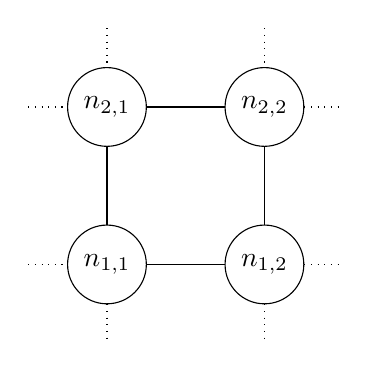
\begin{tikzpicture}
	% Default action for each node
	\tikzstyle{every node}=[draw, shape=circle, minimum size=1cm];

										\coordinate (northleft) at (-1,4);	\coordinate (northright) at (1,4);
	\coordinate (westup) at (-2,3);		\node (n21) at (-1,3) {$n_{2,1}$};	\node (n22) at (1,3) {$n_{2,2}$};	\coordinate (eastup) at (2,3);
	\coordinate (westdown) at (-2,1);	\node (n11) at (-1,1) {$n_{1,1}$};	\node (n12) at (1,1) {$n_{1,2}$};	\coordinate (eastdown) at (2,1);
										\coordinate (southleft) at (-1,0);	\coordinate (southright) at (1,0);

	\draw[outside] (westup) -- (n21);
	\draw (n21) -- (n22);
	\draw[outside] (n22) -- (eastup);

	\draw[outside] (westdown) -- (n11);
	\draw (n11) -- (n12);
	\draw[outside] (n12) -- (eastdown);

	\draw[outside] (northleft) -- (n21);
	\draw (n21) -- (n11);
	\draw[outside] (n11) -- (southleft);

	\draw[outside] (northright) -- (n22);
	\draw (n22) -- (n12);
	\draw[outside] (n12) -- (southright);

\end{tikzpicture}

\end{enumerate}








%%%% Definition A

%% Definition A summary
\section{Function definition: Extend a quad (used in phase 2)}
Starting from $Q_i = \Quad {n_{1,i}} {n_{1,i+1}} {n_{2,i}} {n_{2,i+1}}$, which must be a valid quad in a structured region, we would like to find two more vertices $n_{1, i+2}$ and $n_{2,i+2}$, such that $Q_{i+1} = \Quad {n_{1,i+1}} {n_{1,i+2}} {n_{2,i+1}} {n_{2,i+2}}$ forms a valid quad in a structured quad region. They must satisfy the following constraints:

\begin{itemize}
\item Each of the vertices $n_{1, i+2}$ and $n_{2,i+2}$ must have exactly 4 neighbours.
\item Each of the following pairs of vertices are neighbours: $n_{1,i+1}$~and~$n_{1,i+2}$ ; $n_{2,i+1}$~and~$n_{2,i+2}$ ; $n_{1,i+2}$~and~$n_{2,i+2}$.
\item Each of the vertices $n_{1, i+2}$ and $n_{2,i+2}$ must \emph{not} neighbour any vertex that has been visited thus far, apart from those vertices explicitly mentioned.
\end{itemize}

%% Definition A diagram

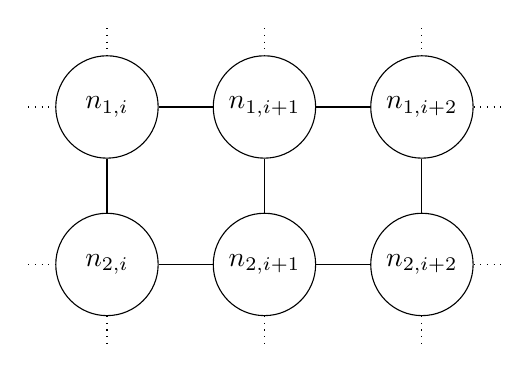
\begin{tikzpicture}[scale=1]
	% Default action for each node
	\tikzstyle{every node}=[draw, shape=circle, minimum size=1.3cm];

										\coordinate (northleft) at (0, 2);	\coordinate (northmid) at (2, 2);		\coordinate (northright) at (4, 2);
	\coordinate (westup) at (-1,1);		\node (r1c1) at (0,1) {$n_{1,i}$};	\node (r1c2) at (2,1) {$n_{1,i+1}$};	\node (r1c3) at (4,1) {$n_{1,i+2}$};	\coordinate (eastup) at (5,1);
	\coordinate (westdown) at (-1,-1);	\node (r2c1) at (0,-1) {$n_{2,i}$};	\node (r2c2) at (2,-1) {$n_{2,i+1}$};	\node (r2c3) at (4,-1) {$n_{2,i+2}$};	\coordinate (eastdown) at (5,-1);
										\coordinate (southleft) at (0, -2);	\coordinate (southmid) at (2, -2);		\coordinate (southright) at (4, -2);

	% Horizontals
	\draw[outside] (westup) -- (r1c1);
	\draw (r1c1) -- (r1c2);
	\draw (r1c2) -- (r1c3);
	\draw[outside] (r1c3) -- (eastup);

	\draw[outside] (westdown) -- (r2c1);
	\draw (r2c1) -- (r2c2);
	\draw (r2c2) -- (r2c3);
	\draw[outside] (r2c3) -- (eastdown);

	% Verticals
	\draw[outside] (northleft) -- (r1c1);
	\draw (r1c1) -- (r2c1);
	\draw[outside] (r2c1) -- (southleft);

	\draw[outside] (northmid) -- (r1c2);
	\draw (r1c2) -- (r2c2);
	\draw[outside] (r2c2) -- (southmid);

	\draw[outside] (northright) -- (r1c3);
	\draw (r1c3) -- (r2c3);
	\draw[outside] (r2c3) -- (southright);
\end{tikzpicture}


%% Definition A algorithm

\subsection{Algorithm}

\begin{enumerate}
\item $n_{1,i+1}$ has 4 neighbours, which include $n_{1,i}$ and $n_{2,i+1}$. Call the remaining 2 neighbours $a$ and $b$. This is expressed by:
$$ \AdjVV(n_{1,i+1}) \setminus \{ n_{1,i} , n_{2,i+1} \} = \{ a , b \} $$

\item $n_{2,i+1}$ has 4 neighbours, which include $n_{2,i}$ and $n_{1,i+1}$. Call the remaining 2 neighbours $c$ and $d$.
$$ \AdjVV(n_{2,i+1}) \setminus \{ n_{2,i} , n_{1,i+1} \} = \{ c , d \} $$

\item Choose two vertices $n_{1,i+2} \in \{ a , b \}$ and $n_{2,i+2} \in \{ c , d \}$ such that $n_{1,i+2}$ and $n_{2,i+2}$ are neighbours, which is expressible\footnote{Or equivalently (by symmetry of $\AdjVV$) $n_{2,i+2} \in \AdjVV(n_{1,i+2})$} as:
$$n_{1,i+2} \in \AdjVV(n_{2,i+2})$$
and such that they each have exactly 4 neighbours. If no such vertices $n_{1,i+2}$ and $n_{2,i+2}$ exist, fail the procedure.


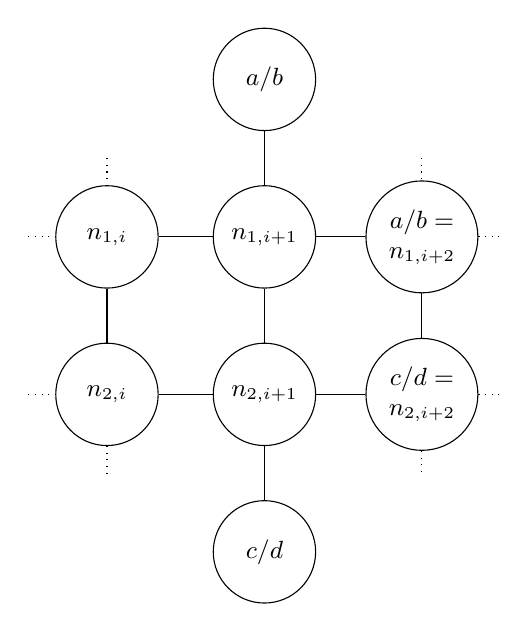
\begin{tikzpicture}[scale=1]
	% Default action for each node
	\tikzstyle{every node}=[draw, shape=circle, minimum size=1.3cm, align=center, font=\small];

										\coordinate (northleft) at (0, 2);	\coordinate (northmid) at (2, 2);		\coordinate (northright) at (4, 2);
	\coordinate (westup) at (-1,3);											\node (abup) at (2,3) {$a/b$};			\coordinate (eastup) at (5,1);
	\coordinate (westmid) at (-1,1);	\node (r1c1) at (0,1) {$n_{1,i}$};	\node (r1c2) at (2,1) {$n_{1,i+1}$};	\node (r1c3) at (4,1) {$a/b =$ \\ $n_{1,i+2}$};		\coordinate (eastmid) at (5,1);
	\coordinate (westdown) at (-1,-1);	\node (r2c1) at (0,-1) {$n_{2,i}$};	\node (r2c2) at (2,-1) {$n_{2,i+1}$};	\node (r2c3) at (4,-1) {$c/d =$ \\ $n_{2,i+2}$};	\coordinate (eastdown) at (5,-1);
	\coordinate (westlow) at (-1,-3);										\node (cdup) at (2,-3) {$c/d$};			\coordinate (eastlow) at (5,1);
										\coordinate (southleft) at (0, -2);	\coordinate (southmid) at (2, -2);		\coordinate (southright) at (4, -2);

	% Horizontals
	\draw[outside] (westmid) -- (r1c1);
	\draw (r1c1) -- (r1c2);
	\draw (r1c2) -- (r1c3);
	\draw[outside] (r1c3) -- (eastmid);

	\draw[outside] (westdown) -- (r2c1);
	\draw (r2c1) -- (r2c2);
	\draw (r2c2) -- (r2c3);
	\draw[outside] (r2c3) -- (eastdown);

	% Verticals
	\draw[outside] (northleft) -- (r1c1);
	\draw (r1c1) -- (r2c1);
	\draw[outside] (r2c1) -- (southleft);

	\draw (abup) -- (r1c2);
	\draw (r1c2) -- (r2c2);
	\draw (r2c2) -- (cdup);

	\draw[outside] (northright) -- (r1c3);
	\draw (r1c3) -- (r2c3);
	\draw[outside] (r2c3) -- (southright);
\end{tikzpicture}


\item If any of the two vertices $n_{1,i+2}$ and $n_{2,i+2}$ exists in $\Visited$, that is $\{ n_{1,i+2} , n_{2,i+2} \} \cap \Visited \neq \varnothing$, fail the procedure.
Otherwise add the two vertices to $\Visited$.

\item Ensure for every vertex $n \in \{ n_{1,i+2} , n_{2,i+2} \}$ that its visited neighbours, $\AdjVV(n) \cap \Visited$, are exactly those explicitly stated above. If this is not the case, remove $\{ n_{1,i+2} , n_{2,i+2} \}$ from $\Visited$ and fail the procedure.

\item Return the two vertices $n_{1,i+2}$ and $n_{2,i+2}$.
\end{enumerate}







%%%% PHASE 2

\section{Phase 2: Extend a row}
%% Phase 2.1 summary
``Extend a quad'' is iteratively applied, starting from $Q_1 = \Qinit$, to yield successive quads until it fails.
The resulting vertices are appended to the \emph{right} of $\Structured$ to form a single quad row in a structured quad region, or equivalently a successive pair of node rows.

%% Phase 2.1 diagram
\begin{tikzpicture}[scale=1]
	% Default action for each node
	\tikzstyle{every node}=[draw, shape=circle, minimum size=1.3cm];

	% MIDDLE

										\coordinate (northleft) at (0, 2);	\coordinate (northright) at (2, 2);
	\coordinate (westup) at (-1,1);		\node (r1c1) at (0,1) {$n_{1,1}$};	\node (r1c2) at (2,1) {$n_{1,2}$};		\coordinate (eastup) at (3,1);
	\coordinate (westdown) at (-1,-1);	\node (r2c1) at (0,-1) {$n_{2,1}$};	\node (r2c2) at (2,-1) {$n_{2,2}$};		\coordinate (eastdown) at (3,-1);
										\coordinate (southleft) at (0, -2);	\coordinate (southright) at (2, -2);

	% ellipses
	\coordinate (ellipsis westup) at (4,1);		\coordinate (ellipsis eastup) at (4.5,1);
	\coordinate (ellipsis westdown) at (4,-1);	\coordinate (ellipsis eastdown) at (4.5,-1);


	% RHS
											\coordinate (rhs north) at (6, 2);
	\coordinate (rhs westup) at (5,1);		\node (r1cn) at (6,1) {$n_{1,c_+}$};	\coordinate (rhs eastup) at (7,1);
	\coordinate (rhs westdown) at (5,-1);	\node (r2cn) at (6,-1) {$n_{2,c_+}$};	\coordinate (rhs eastdown) at (7,-1);
											\coordinate (rhs south) at (6, -2);



	% Horizontals
	\draw[outside] (westup) -- (r1c1);
	\draw (r1c1) -- (r1c2);
	\draw (r1c2) -- (r1c3);
	\draw (r1c3) -- (eastup);

	\draw[outside] (westdown) -- (r2c1);
	\draw (r2c1) -- (r2c2);
	\draw (r2c2) -- (r2c3);
	\draw (r2c3) -- (eastdown);

	\draw[ellipsis] (ellipsis westup) -- (ellipsis eastup);
	\draw[ellipsis] (ellipsis westdown) -- (ellipsis eastdown);


	\draw (rhs westup) -- (r1cn);
	\draw[outside] (r1cn) -- (rhs eastup);

	\draw (rhs westdown) -- (r2cn);
	\draw[outside] (r2cn) -- (rhs eastdown);

	% Verticals
	\draw[outside] (northleft) -- (r1c1);
	\draw (r1c1) -- (r2c1);
	\draw[outside] (r2c1) -- (southleft);

	\draw[outside] (northright) -- (r1c2);
	\draw (r1c2) -- (r2c2);
	\draw[outside] (r2c2) -- (southright);

	\draw[outside] (rhs north) -- (r1cn);
	\draw (r1cn) -- (r2cn);
	\draw[outside] (r2cn) -- (rhs south);
\end{tikzpicture}



%% Phase 2.2 summary
Next, ``Extend a quad'' is again iteratively applied, this time with $Q_1 = \Qinitmirror$, the mirror image of $Q_{init}$ about the y-axis.
The repeated application yields successive quads until the procedure fails.
The resulting vertices are appended to the \emph{left} of $\Structured$ to extend the existing quad row, or equivalently a successive pair of node rows.


%% Phase 2.2 diagram
\begin{tikzpicture}[scale=1]
	% Default action for each node
	\tikzstyle{every node}=[draw, shape=circle, minimum size=1.3cm];

	% LHS
												\coordinate (lhs north) at (-3.5, 2);
	\coordinate (lhs westup) at (-4.5,1);		\node (r1cm) at (-3.5,1) {$n_{1,c_{\!^{\_}}}$};		\coordinate (lhs eastup) at (-2.5,1);
	\coordinate (lhs westdown) at (-4.5,-1);	\node (r2cm) at (-3.5,-1) {$n_{2,c_{\!^{\_}}}$};	\coordinate (lhs eastdown) at (-2.5,-1);
												\coordinate (lhs south) at (-3.5, -2);

	% lhs ellipses
	\coordinate (lhs ellipsis westup) at (-2,1);	\coordinate (lhs ellipsis eastup) at (-1.5,1);
	\coordinate (lhs ellipsis westdown) at (-2,-1);	\coordinate (lhs ellipsis eastdown) at (-1.5,-1);


	% MIDDLE
										\coordinate (northleft) at (0, 2);	\coordinate (northright) at (2, 2);
	\coordinate (westup) at (-1,1);		\node (r1c1) at (0,1) {$n_{1,1}$};	\node (r1c2) at (2,1) {$n_{1,2}$};		\coordinate (eastup) at (3,1);
	\coordinate (westdown) at (-1,-1);	\node (r2c1) at (0,-1) {$n_{2,1}$};	\node (r2c2) at (2,-1) {$n_{2,2}$};		\coordinate (eastdown) at (3,-1);
										\coordinate (southleft) at (0, -2);	\coordinate (southright) at (2, -2);

	% rhs ellipses
	\coordinate (rhs ellipsis westup) at (4,1);		\coordinate (rhs ellipsis eastup) at (4.5,1);
	\coordinate (rhs ellipsis westdown) at (4,-1);	\coordinate (rhs ellipsis eastdown) at (4.5,-1);


	% RHS
											\coordinate (rhs north) at (6, 2);
	\coordinate (rhs westup) at (5,1);		\node (r1cn) at (6,1) {$n_{1,c_+}$};	\coordinate (rhs eastup) at (7,1);
	\coordinate (rhs westdown) at (5,-1);	\node (r2cn) at (6,-1) {$n_{2,c_+}$};	\coordinate (rhs eastdown) at (7,-1);
											\coordinate (rhs south) at (6, -2);



	% Horizontals
	\draw (westup) -- (r1c1);
	\draw (r1c1) -- (r1c2);
	\draw (r1c2) -- (r1c3);
	\draw (r1c3) -- (eastup);

	\draw(westdown) -- (r2c1);
	\draw (r2c1) -- (r2c2);
	\draw (r2c2) -- (r2c3);
	\draw (r2c3) -- (eastdown);


	\draw[ellipsis] (rhs ellipsis westup) -- (rhs ellipsis eastup);
	\draw[ellipsis] (rhs ellipsis westdown) -- (rhs ellipsis eastdown);

	\draw (rhs westup) -- (r1cn);
	\draw[outside] (r1cn) -- (rhs eastup);

	\draw (rhs westdown) -- (r2cn);
	\draw[outside] (r2cn) -- (rhs eastdown);


	\draw[ellipsis] (lhs ellipsis westup) -- (lhs ellipsis eastup);
	\draw[ellipsis] (lhs ellipsis westdown) -- (lhs ellipsis eastdown);

	\draw (r1cm) -- (lhs eastup);
	\draw[outside] (lhs westup) -- (r1cm);

	\draw[outside] (lhs westdown) -- (r2cm);
	\draw (r2cm) -- (lhs eastdown);


	% Verticals
	\draw[outside] (northleft) -- (r1c1);
	\draw (r1c1) -- (r2c1);
	\draw[outside] (r2c1) -- (southleft);

	\draw[outside] (northright) -- (r1c2);
	\draw (r1c2) -- (r2c2);
	\draw[outside] (r2c2) -- (southright);


	\draw[outside] (rhs north) -- (r1cn);
	\draw (r1cn) -- (r2cn);
	\draw[outside] (r2cn) -- (rhs south);


	\draw[outside] (lhs north) -- (r1cm);
	\draw (r1cm) -- (r2cm);
	\draw[outside] (r2cm) -- (lhs south);
\end{tikzpicture}












%% Phase 2 algorithm

\subsection{Algorithm}

\paragraph{Extend to the right}
\begin{enumerate}
\item Let $Q_{in} = Q_{init} = \Qinit$, as produced by ``Grow a quad''.
\item \label{step:extend_quad} Let $\Quad {n_{1,i}} {n_{1,i+1}} {n_{2,i}} {n_{2,i+1}}$ represent the elements of $Q_{in}$.
\item Call the procedure ``Extend a quad'' with $Q_{in}$ as input.
\item If the procedure fails, go to step~\ref{step:init_reverse}.
\item Otherwise, append the two new vertices obtained, $n_{1,i+2}$ and $n_{2,i+2}$ to the \emph{right} of $\Structured$. \\
Thus $\Structured$ will become:
	$\begin{bmatrix}
	n_{1,1} & n_{1,2} & \cdots  & n_{1,i} & n_{1,i+1} & n_{1,i+2} \\
	n_{2,1} & n_{2,2} & \cdots  & n_{2,i} & n_{2,i+1} & n_{2,i+2}
	\end{bmatrix}$

\item Set $Q_{in} = \Quad {n_{1,i+1}} {n_{1,i+2}} {n_{2,i+1}} {n_{2,i+2}}$, and continue from step~\ref{step:extend_quad}.

\end{enumerate}
\paragraph{Extend to the left}
\begin{enumerate}[resume]

% Reverse
\item \label{step:init_reverse} Let $Q_{in} = \Qinitmirror$ be the mirror image of $Q_{init}$ about the y-axis.



\item \label{step:reverse_extend_quad} Let $\Quad {n_{1,i}} {n_{1,i+1}} {n_{2,i}} {n_{2,i+1}}$ represent the elements of $Q_{in}$.
\item Call the procedure ``Extend a quad'' with $Q_{in}$ as input.
\item If the procedure fails, return immediately.
\item Otherwise, append the two new vertices obtained, $n_{1,i+2}$ and $n_{2,i+2}$ to the \emph{left} of $\Structured$. \\
Thus $\Structured$ will become:
	$\begin{bmatrix}
	n_{1,i+2} & n_{1,i+1} & n_{1,i} & \cdots & n_{1,1} & n_{1,2} & \cdots  & n_{1,c} \\
	n_{2,i+2} & n_{2,i+1} & n_{2,i} & \cdots & n_{2,1} & n_{2,2} & \cdots  & n_{2,c}
	\end{bmatrix}$
where $n_{1,c}$ and $n_{2,c}$ denote the rightmost vertices in $\Structured$.

\item Set $Q_{in} = \Quad {n_{1,i+1}} {n_{1,i+2}} {n_{2,i+1}} {n_{2,i+2}}$, and continue from step~\ref{step:reverse_extend_quad}.
\end{enumerate}





%%%% Definition B

\section{Function definition: Extend rows (used in phase 3)}
%% Definition B summary
We are given a quad row in a structured quad region, that is a pair of successive node rows, call them $r_i$ and $r_{i+1}$.
The nodes in each row are denoted by $n_{i,1} \cdots n_{i,c}$ and $n_{i+1,1} \cdots n_{i+1,c}$, respectively, where $c >= 3$ is the number of node columns.

We extend this pair of node rows $r_i$ and $r_{i+1}$ by a third node row, $r_{i+2}$, consisting of nodes $n_{i+2,1} \cdots n_{i+2,c}$. These must satisfy the following conditions:

\begin{itemize}
\item Each vertex $n_{i+2,j}$ for $j \in [1..c]$ must have exactly four neighbours.
\item Each of the pairs of vertices $n_{i+2,j}$ and $n_{i+2,j+1}$ for $j \in [1..c-1]$ are neighbours.
\item Each of the pairs of vertices $n_{i+1,j}$ and $n_{i+2,j}$ for $j \in [1..c]$ are neighbours.
\item Each vertex $n_{i+2,j}$ for $j \in [1..c]$ must not neighbour any vertex that has been visited thus far, apart from those vertices explicitly mentioned.
\end{itemize}


%% Definition B diagram
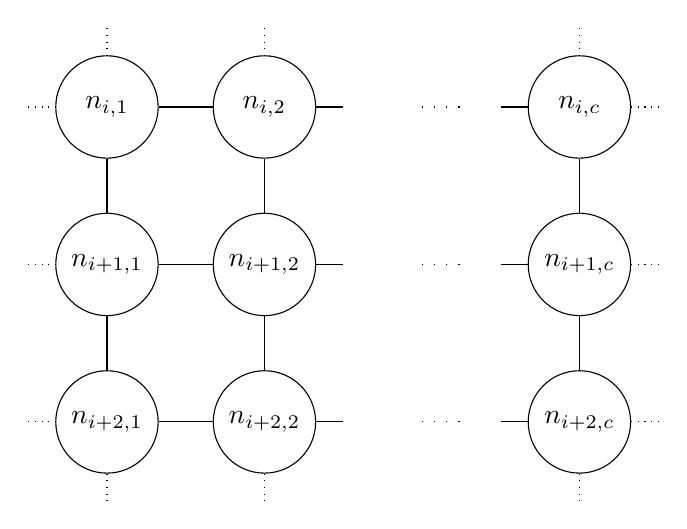
\begin{tikzpicture}[scale=1]
	% Default action for each node
	\tikzstyle{every node}=[draw, shape=circle, minimum size=1.3cm];

	% MIDDLE

										\coordinate (northleft) at (0, 2);		\coordinate (northright) at (2, 2);
	\coordinate (westup) at (-1,1);		\node (r1c1) at (0,1) {$n_{i,1}$};		\node (r1c2) at (2,1) {$n_{i,2}$};		\coordinate (eastup) at (3,1);
	\coordinate (westmid) at (-1,-1);	\node (r2c1) at (0,-1) {$n_{i+1,1}$};	\node (r2c2) at (2,-1) {$n_{i+1,2}$};	\coordinate (eastmid) at (3,-1);
	\coordinate (westdown) at (-1,-3);	\node (r3c1) at (0,-3) {$n_{i+2,1}$};	\node (r3c2) at (2,-3) {$n_{i+2,2}$};	\coordinate (eastdown) at (3,-3);
										\coordinate (southleft) at (0, -4);		\coordinate (southright) at (2, -4);

	% ellipses
	\coordinate (ellipsis westup) at (4,1);		\coordinate (ellipsis eastup) at (4.5,1);
	\coordinate (ellipsis westmid) at (4,-1);	\coordinate (ellipsis eastmid) at (4.5,-1);
	\coordinate (ellipsis westdown) at (4,-3);	\coordinate (ellipsis eastdown) at (4.5,-3);


	% RHS
											\coordinate (rhs north) at (6, 2);
	\coordinate (rhs westup) at (5,1);		\node (r1cn) at (6,1) {$n_{i,c}$};		\coordinate (rhs eastup) at (7,1);
	\coordinate (rhs westmid) at (5,-1);	\node (r2cn) at (6,-1) {$n_{i+1,c}$};	\coordinate (rhs eastmid) at (7,-1);
	\coordinate (rhs westdown) at (5,-3);	\node (r3cn) at (6,-3) {$n_{i+2,c}$};	\coordinate (rhs eastdown) at (7,-3);
											\coordinate (rhs south) at (6, -4);

	% Horizontals
	\draw[outside] (westup) -- (r1c1);
	\draw (r1c1) -- (r1c2);
	\draw (r1c2) -- (eastup);

	\draw[outside] (westmid) -- (r2c1);
	\draw (r2c1) -- (r2c2);
	\draw (r2c2) -- (eastmid);

	\draw[outside] (westdown) -- (r3c1);
	\draw (r3c1) -- (r3c2);
	\draw (r3c2) -- (eastdown);


	\draw[ellipsis] (ellipsis westup) -- (ellipsis eastup);
	\draw[ellipsis] (ellipsis westmid) -- (ellipsis eastmid);
	\draw[ellipsis] (ellipsis westdown) -- (ellipsis eastdown);


	\draw (rhs westup) -- (r1cn);
	\draw[outside] (r1cn) -- (rhs eastup);

	\draw (rhs westmid) -- (r2cn);
	\draw[outside] (r2cn) -- (rhs eastmid);

	\draw (rhs westdown) -- (r3cn);
	\draw[outside] (r3cn) -- (rhs eastdown);

	% Verticals
	\draw[outside] (northleft) -- (r1c1);
	\draw (r1c1) -- (r2c1);
	\draw (r2c1) -- (r3c1);
	\draw[outside] (r3c1) -- (southleft);

	\draw[outside] (northright) -- (r1c2);
	\draw (r1c2) -- (r2c2);
	\draw (r2c2) -- (r3c2);
	\draw[outside] (r3c2) -- (southright);

	\draw[outside] (rhs north) -- (r1cn);
	\draw (r1cn) -- (r2cn);
	\draw (r2cn) -- (r3cn);
	\draw[outside] (r3cn) -- (rhs south);
\end{tikzpicture}



%% Definition B algorithm

\subsection{Algorithm}

\begin{enumerate}
\item Let $n_{i+2,2}$ be the unique vertex in the set $\AdjVV(n_{i+1,2}) \setminus \{ n_{i+1,1} , n_{i+1,3} , n_{i,2} \} $.
\item Let $N = \AdjVV(n_{i+1,1}) \cap \AdjVV(n_{i+2,2})$ be the common neighbours of $n_{i+1,1}$ and $n_{i+2,2}$.
If the number of common neighbours $\card{N}$ is not exactly two, fail the procedure.
\item We know that $n_{i+1,2} \in N$ by construction. Let $n_{i+2,1}$ be the other vertex in $N$.
\item If either of $n_{i+2,1}$ or $n_{i+2,2}$ is in $\Visited$, fail the procedure. Otherwise add the two vertices to $\Visited$.
\item Ensure that the visited neighbours of $n_{i+2,1}$ and $n_{i+2,2}$ are exactly as specified,
that is $n_{i+2,1} \cap \Visited = \{ n_{i+2,2} , n_{i+1,1} \}$ and $n_{i+2,2} \cap \Visited = \{ n_{i+2,1} , n_{i+1,2} \}$.
If this is not the case, remove $n_{i+2,1}$ and $n_{i+2,2}$ from $\Visited$ and fail the procedure.





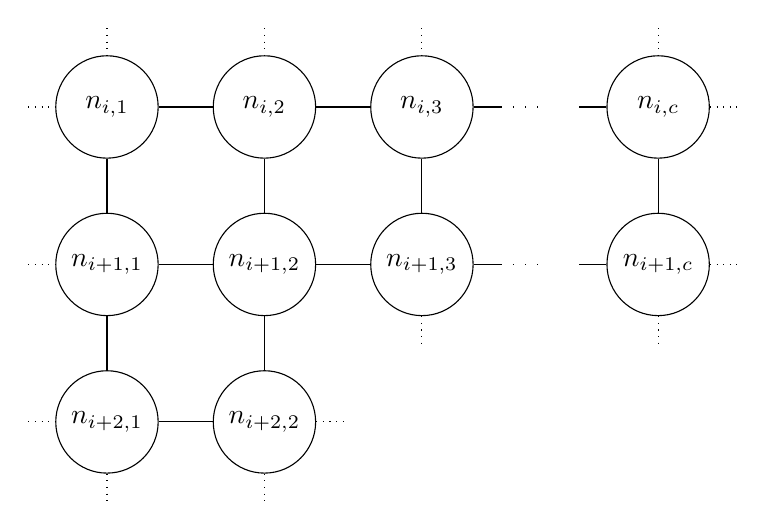
\begin{tikzpicture}[scale=1]
	% Default action for each node
	\tikzstyle{every node}=[draw, shape=circle, minimum size=1.3cm];

	% MIDDLE

										\coordinate (northleft) at (0, 2);		\coordinate (northmid) at (2, 2);		\coordinate (northright) at (4, 2);
	\coordinate (westup) at (-1,1);		\node (r1c1) at (0,1) {$n_{i,1}$};		\node (r1c2) at (2,1) {$n_{i,2}$};		\node (r1c3) at (4,1) {$n_{i,3}$};		\coordinate (eastup) at (5,1);
	\coordinate (westmid) at (-1,-1);	\node (r2c1) at (0,-1) {$n_{i+1,1}$};	\node (r2c2) at (2,-1) {$n_{i+1,2}$};	\node (r2c3) at (4,-1) {$n_{i+1,3}$};	\coordinate (eastmid) at (5,-1);
	\coordinate (westdown) at (-1,-3);	\node (r3c1) at (0,-3) {$n_{i+2,1}$};	\node (r3c2) at (2,-3) {$n_{i+2,2}$};											\coordinate (eastdown) at (3,-3);
										\coordinate (southleft) at (0, -4);		\coordinate (southmid) at (2, -4);		\coordinate (southright) at (4, -2);

	% ellipses
	\coordinate (ellipsis westup) at (5,1);		\coordinate (ellipsis eastup) at (5.5,1);
	\coordinate (ellipsis westdown) at (5,-1);	\coordinate (ellipsis eastdown) at (5.5,-1);


	% RHS
											\coordinate (rhs north) at (7, 2);
	\coordinate (rhs westup) at (6,1);		\node (r1cn) at (7,1) {$n_{i,c}$};		\coordinate (rhs eastup) at (8,1);
	\coordinate (rhs westmid) at (6,-1);	\node (r2cn) at (7,-1) {$n_{i+1,c}$};	\coordinate (rhs eastmid) at (8,-1);
											\coordinate (rhs south) at (7, -2);

	% Horizontals
	\draw[outside] (westup) -- (r1c1);
	\draw (r1c1) -- (r1c2) -- (r1c3) -- (eastup);

	\draw[outside] (westmid) -- (r2c1);
	\draw (r2c1) -- (r2c2) -- (r2c3) -- (eastmid);

	\draw[outside] (westdown) -- (r3c1);
	\draw (r3c1) -- (r3c2);
	\draw[outside] (r3c2) -- (eastdown);


	\draw[ellipsis] (ellipsis westup) -- (ellipsis eastup);
	\draw[ellipsis] (ellipsis westdown) -- (ellipsis eastdown);


	\draw (rhs westup) -- (r1cn);
	\draw[outside] (r1cn) -- (rhs eastup);

	\draw (rhs westmid) -- (r2cn);
	\draw[outside] (r2cn) -- (rhs eastmid);


	% Verticals
	\draw[outside] (northleft) -- (r1c1);
	\draw (r1c1) -- (r2c1);
	\draw (r2c1) -- (r3c1);
	\draw[outside] (r3c1) -- (southleft);

	\draw[outside] (northmid) -- (r1c2);
	\draw (r1c2) -- (r2c2);
	\draw (r2c2) -- (r3c2);
	\draw[outside] (r3c2) -- (southmid);

	\draw[outside] (northright) -- (r1c3);
	\draw (r1c3) -- (r2c3);
	\draw[outside] (r2c3) -- (southright);


	\draw[outside] (rhs north) -- (r1cn);
	\draw (r1cn) -- (r2cn);
	\draw[outside] (r2cn) -- (rhs south);
\end{tikzpicture}




\item For each column\footnote{Possibly none if $c = 3$} $j \in [3..c-1]$:
	\begin{enumerate}
	\item Let $n_{i+2,j}$ be the unique vertex in the set $\AdjVV(n_{i+1,j}) \setminus \{ n_{i+1,j-1} , n_{i+1,j+1} , n_{i,j} \}$.
	\item If $n_{i+2,j} \in \Visited$, remove all vertices in $r_{i+2}$ from $\Visited$, that is $\{ n_{i+2,k} \mid k \in [1..j] \}$ and fail the procedure.
	Otherwise, add $n_{i+2,j}$ $\Visited$.
	\item Ensure that visited neighbours of $n_{i+2,j}$ are exactly $n_{i+2,j-1}$, $n_{i+1,j}$.
	If this is not the case remove vertices $\{ n_{i+2,k} \mid k \in [1..j] \}$ from $\Visited$ and fail the procedure.
	\end{enumerate}




% Foreach j diagram
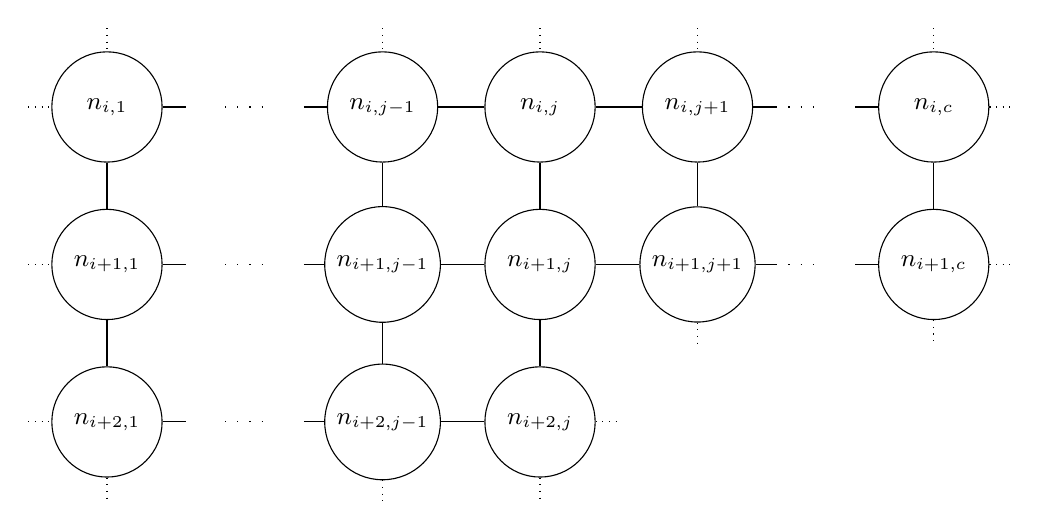
\begin{tikzpicture}[scale=1]
	% Default action for each node
	\tikzstyle{every node}=[draw, shape=circle, minimum size=1.4cm, font=\small];

	% LHS
												\coordinate (lhs north) at (-3.5, 2);
	\coordinate (lhs westup) at (-4.5,1);		\node (r1c0) at (-3.5,1) {$n_{i,1}$};		\coordinate (lhs eastup) at (-2.5,1);
	\coordinate (lhs westmid) at (-4.5,-1);		\node (r2c0) at (-3.5,-1) {$n_{i+1,1}$};	\coordinate (lhs eastmid) at (-2.5,-1);
	\coordinate (lhs westdown) at (-4.5,-3);	\node (r3c0) at (-3.5,-3) {$n_{i+2,1}$};	\coordinate (lhs eastdown) at (-2.5,-3);
												\coordinate (lhs south) at (-3.5, -4);

	% LHS ellipses
	\coordinate (lhs ellipsis westup) at (-2,1);	\coordinate (lhs ellipsis eastup) at (-1.5,1);
	\coordinate (lhs ellipsis westmid) at (-2,-1);	\coordinate (lhs ellipsis eastmid) at (-1.5,-1);
	\coordinate (lhs ellipsis westdown) at (-2,-3);	\coordinate (lhs ellipsis eastdown) at (-1.5,-3);


	% MIDDLE
										\coordinate (northleft) at (0, 2);		\coordinate (northmid) at (2, 2);		\coordinate (northright) at (4, 2);
	\coordinate (westup) at (-1,1);		\node (r1c1) at (0,1) {$n_{i,j-1}$};	\node (r1c2) at (2,1) {$n_{i,j}$};		\node (r1c3) at (4,1) {$n_{i,j+1}$};	\coordinate (eastup) at (5,1);
	\coordinate (westmid) at (-1,-1);	\node (r2c1) at (0,-1) {$n_{i+1,j-1}$};	\node (r2c2) at (2,-1) {$n_{i+1,j}$};	\node (r2c3) at (4,-1) {$n_{i+1,j+1}$};	\coordinate (eastmid) at (5,-1);
	\coordinate (westdown) at (-1,-3);	\node (r3c1) at (0,-3) {$n_{i+2,j-1}$};	\node (r3c2) at (2,-3) {$n_{i+2,j}$};											\coordinate (eastdown) at (3,-3);
										\coordinate (southleft) at (0, -4);		\coordinate (southmid) at (2, -4);		\coordinate (southright) at (4, -2);

	% rhs ellipses
	\coordinate (rhs ellipsis westup) at (5,1);		\coordinate (rhs ellipsis eastup) at (5.5,1);
	\coordinate (rhs ellipsis westdown) at (5,-1);	\coordinate (rhs ellipsis eastdown) at (5.5,-1);


	% RHS
											\coordinate (rhs north) at (7, 2);
	\coordinate (rhs westup) at (6,1);		\node (r1cn) at (7,1) {$n_{i,c}$};		\coordinate (rhs eastup) at (8,1);
	\coordinate (rhs westmid) at (6,-1);	\node (r2cn) at (7,-1) {$n_{i+1,c}$};	\coordinate (rhs eastmid) at (8,-1);
											\coordinate (rhs south) at (7, -2);

	% Horizontals
	\draw[outside] (lhs westup) -- (r1c0);
	\draw (r1c0) -- (lhs eastup);

	\draw[outside] (lhs westmid) -- (r2c0);
	\draw (r2c0) -- (lhs eastmid);

	\draw[outside] (lhs westdown) -- (r3c0);
	\draw (r3c0) -- (lhs eastdown);


	\draw (westup) -- (r1c1) -- (r1c2) -- (r1c3) -- (eastup);

	\draw (westmid) -- (r2c1) -- (r2c2) -- (r2c3) -- (eastmid);

	\draw (westdown) -- (r3c1) -- (r3c2);
	\draw[outside] (r3c2) -- (eastdown);


	\draw[ellipsis] (lhs ellipsis westup) -- (lhs ellipsis eastup);
	\draw[ellipsis] (lhs ellipsis westmid) -- (lhs ellipsis eastmid);
	\draw[ellipsis] (lhs ellipsis westdown) -- (lhs ellipsis eastdown);

	\draw[ellipsis] (rhs ellipsis westup) -- (rhs ellipsis eastup);
	\draw[ellipsis] (rhs ellipsis westdown) -- (rhs ellipsis eastdown);


	\draw (rhs westup) -- (r1cn);
	\draw[outside] (r1cn) -- (rhs eastup);

	\draw (rhs westmid) -- (r2cn);
	\draw[outside] (r2cn) -- (rhs eastmid);


	% Verticals
	\draw[outside] (lhs north) -- (r1c0);
	\draw (r1c0) -- (r2c0) -- (r3c0);
	\draw[outside] (r3c0) -- (lhs south);


	\draw[outside] (northleft) -- (r1c1);
	\draw (r1c1) -- (r2c1) -- (r3c1);
	\draw[outside] (r3c1) -- (southleft);

	\draw[outside] (northmid) -- (r1c2);
	\draw (r1c2) -- (r2c2) -- (r3c2);
	\draw[outside] (r3c2) -- (southmid);

	\draw[outside] (northright) -- (r1c3);
	\draw (r1c3) -- (r2c3);
	\draw[outside] (r2c3) -- (southright);


	\draw[outside] (rhs north) -- (r1cn);
	\draw (r1cn) -- (r2cn);
	\draw[outside] (r2cn) -- (rhs south);
\end{tikzpicture}







\item Consider $\AdjVV(n_{i+2,c-1}) \cap \AdjVV(n_{i+1,c})$, the common neighbours of $n_{i+2,c-1}$ and $n_{i+1,c}$.
If these are not exactly two neighbours, remove vertices $\{ n_{i+2,k} \mid k \in [1..c-1] \}$ from $\Visited$ and fail the procedure.
\item One of the two neighbours must be $n_{i+1,c}$ by construction. Let $n_{i+2,c}$ denote the other neighbour.
\item If $n_{i+2,c} \in \Visited$, remove vertices $\{ n_{i+2,k} \mid k \in [1..c-1] \}$ from $\Visited$ and fail the procedure.
Otherwise, add $n_{i+2,c}$ to $\Visited$.
\item Ensure that the visited neighbours of $n_{i+2,c}$ are exactly $\{ n_{i+2,c-1} , n_{i+1,c} \}$,
that is $\AdjVV(n_{i+2,c}) \cap \Visited = \{ n_{i+2,c-1} , n_{i+1,c} \}$. If this is not the case remove vertices $\{ n_{i+2,k} \mid k \in [1..c] \}$ from $\Visited$ and fail the procedure.




% lastnode diagram
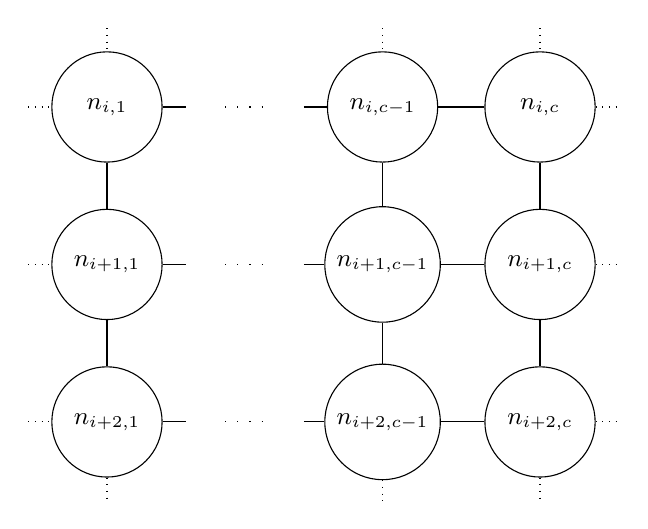
\begin{tikzpicture}[scale=1]
	% Default action for each node
	\tikzstyle{every node}=[draw, shape=circle, minimum size=1.4cm, font=\small];

	% LHS
												\coordinate (lhs north) at (-1.5, 2);
	\coordinate (lhs westup) at (-2.5,1);		\node (r1c0) at (-1.5,1) {$n_{i,1}$};		\coordinate (lhs eastup) at (-0.5,1);
	\coordinate (lhs westmid) at (-2.5,-1);		\node (r2c0) at (-1.5,-1) {$n_{i+1,1}$};	\coordinate (lhs eastmid) at (-0.5,-1);
	\coordinate (lhs westdown) at (-2.5,-3);	\node (r3c0) at (-1.5,-3) {$n_{i+2,1}$};	\coordinate (lhs eastdown) at (-0.5,-3);
												\coordinate (lhs south) at (-1.5, -4);

	% LHS ellipses
	\coordinate (lhs ellipsis westup) at (0,1);		\coordinate (lhs ellipsis eastup) at (0.5,1);
	\coordinate (lhs ellipsis westmid) at (0,-1);	\coordinate (lhs ellipsis eastmid) at (0.5,-1);
	\coordinate (lhs ellipsis westdown) at (0,-3);	\coordinate (lhs ellipsis eastdown) at (0.5,-3);


	% MIDDLE
										\coordinate (northmid) at (2, 2);		\coordinate (northright) at (4, 2);
	\coordinate (westup) at (1,1);		\node (r1c2) at (2,1) {$n_{i,c-1}$};	\node (r1c3) at (4,1) {$n_{i,c}$};		\coordinate (eastup) at (5,1);
	\coordinate (westmid) at (1,-1);	\node (r2c2) at (2,-1) {$n_{i+1,c-1}$};	\node (r2c3) at (4,-1) {$n_{i+1,c}$};	\coordinate (eastmid) at (5,-1);
	\coordinate (westdown) at (1,-3);	\node (r3c2) at (2,-3) {$n_{i+2,c-1}$};	\node (r3c3) at (4,-3) {$n_{i+2,c}$};	\coordinate (eastdown) at (5,-3);
										\coordinate (southmid) at (2, -4);		\coordinate (southright) at (4, -4);




	% Horizontals
	\draw[outside] (lhs westup) -- (r1c0);
	\draw (r1c0) -- (lhs eastup);

	\draw[outside] (lhs westmid) -- (r2c0);
	\draw (r2c0) -- (lhs eastmid);

	\draw[outside] (lhs westdown) -- (r3c0);
	\draw (r3c0) -- (lhs eastdown);


	\draw (westup) -- (r1c2) -- (r1c3);
	\draw[outside] (r1c3) -- (eastup);

	\draw (westmid) -- (r2c2) -- (r2c3);
	\draw[outside] (r2c3) -- (eastmid);

	\draw (westdown) -- (r3c2) -- (r3c3);
	\draw[outside] (r3c3) -- (eastdown);


	\draw[ellipsis] (lhs ellipsis westup) -- (lhs ellipsis eastup);
	\draw[ellipsis] (lhs ellipsis westmid) -- (lhs ellipsis eastmid);
	\draw[ellipsis] (lhs ellipsis westdown) -- (lhs ellipsis eastdown);


	% Verticals
	\draw[outside] (lhs north) -- (r1c0);
	\draw (r1c0) -- (r2c0) -- (r3c0);
	\draw[outside] (r3c0) -- (lhs south);

	\draw[outside] (northmid) -- (r1c2);
	\draw (r1c2) -- (r2c2) -- (r3c2);
	\draw[outside] (r3c2) -- (southmid);

	\draw[outside] (northright) -- (r1c3);
	\draw (r1c3) -- (r2c3) -- (r3c3);
	\draw[outside] (r3c3) -- (southright);

\end{tikzpicture}

\item Return the vertices of node row $r_{i+2}$, that is $n_{i+2,1} \cdots n_{i+2,c}$.
\end{enumerate}





%%%% PHASE 3

\section{Phase 3: Extend rows}
%% Phase 3.1 summary
``Extend a row'' is iteratively applied, starting from $r_1 = n_{1,1} \cdots n_{1,c}$ and $r_2 = n_{2,1} \cdots n_{2,c}$, to yield successive rows until it fails.
The resulting rows are appended \emph{below} $\Structured$.


%% Phase 3.1 diagram
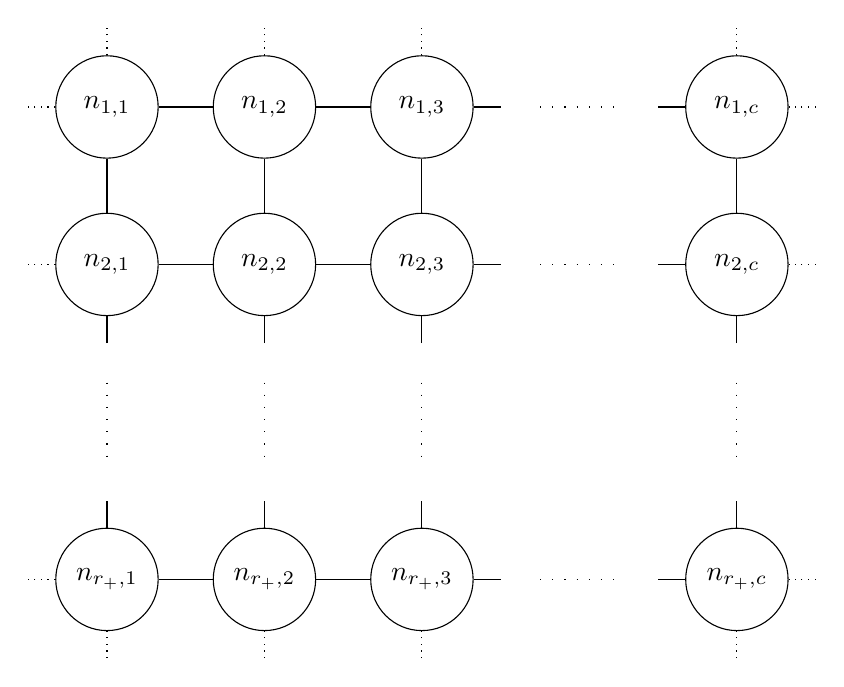
\begin{tikzpicture}
	\tikzstyle{every node}=[draw, shape=circle, minimum size=1.3cm];

	% First rows
	\drawellipsiscol{num=2, rowoffset=6, coloffset=7.5}
	\drawgrid{rows=2, cols=3, rowoffset=6,
		labeler=\plainlabelnode, labelerA=0, labelerB=0,
		southborder=structured, eastborder=structured}
	\drawgrid{rows=2, cols=1, rowoffset=6, coloffset=8,
		labeler=\varcollabelnode, labelerA=0, labelerB=0, labelerC=c,
		southborder=structured, westborder=structured}

	% Bottom horizontal ellipsis
	\drawellipsisrow{num=3, rowoffset=0.5}
	\drawellipsisrow{num=1, rowoffset=0.5, coloffset=8}

	% Last row
	\drawellipsiscol{num=1, rowoffset=0, coloffset=7.5}
	\drawgrid{rows=1, cols=3, rowoffset=0,
		labeler=\varrowlabelnode, labelerA=0, labelerB=0, labelerC=r_+,
		northborder=structured, eastborder=structured}
	\drawgrid{rows=1, cols=1, rowoffset=0, coloffset=8,
		labeler=\varlabelnode, labelerA=0, labelerB=0, labelerC=r_+, labelerD=c,
		northborder=structured, westborder=structured}
\end{tikzpicture}




%% Phase 3.2 summary
``Extend a row'' is iteratively applied, starting from the mirror image of the initial rows about the x-axis, that is $r_1 = n_{2,1} \cdots n_{2,c}$ and $r_2 = n_{1,1} \cdots n_{1,c}$, to yield successive rows until it fails.
The resulting rows are appended \emph{above} $\Structured$.

%% Phase 3.2 diagram
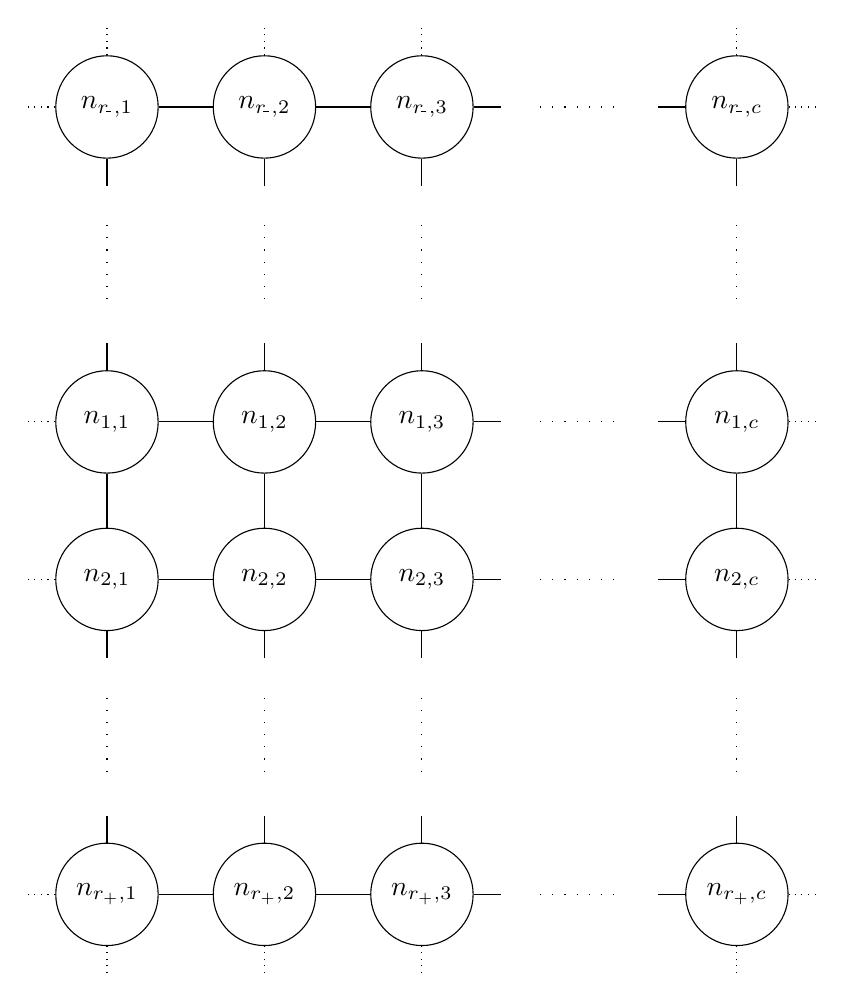
\begin{tikzpicture}
	\tikzstyle{every node}=[draw, shape=circle, minimum size=1.3cm];

	% First first rows
	\drawellipsiscol{num=1, rowoffset=10, coloffset=7.5}
	\drawgrid{rows=1, cols=3, rowoffset=10,
		labeler=\varrowlabelnode, labelerA=0, labelerB=0, labelerC=r_{\!^{\_}},
		southborder=structured, eastborder=structured}
	\drawgrid{rows=1, cols=1, rowoffset=10, coloffset=8,
		labeler=\varlabelnode, labelerA=0, labelerB=0, labelerC=r_{\!^{\_}}, labelerD=c,
		southborder=structured, westborder=structured}

	% Top horizontal ellipsis
	\drawellipsisrow{num=3, rowoffset=6.5}
	\drawellipsisrow{num=1, rowoffset=6.5, coloffset=8}

	% First rows
	\drawellipsiscol{num=2, rowoffset=6, coloffset=7.5}
	\drawgrid{rows=2, cols=3, rowoffset=6,
		labeler=\plainlabelnode, labelerA=0, labelerB=0,
		southborder=structured, eastborder=structured, northborder=structured}
	\drawgrid{rows=2, cols=1, rowoffset=6, coloffset=8,
		labeler=\varcollabelnode, labelerA=0, labelerB=0, labelerC=c,
		southborder=structured, westborder=structured, northborder=structured}

	% Bottom horizontal ellipsis
	\drawellipsisrow{num=3, rowoffset=0.5}
	\drawellipsisrow{num=1, rowoffset=0.5, coloffset=8}

	% Last row
	\drawellipsiscol{num=1, rowoffset=0, coloffset=7.5}
	\drawgrid{rows=1, cols=3, rowoffset=0,
		labeler=\varrowlabelnode, labelerA=0, labelerB=0, labelerC=r_+,
		northborder=structured, eastborder=structured}
	\drawgrid{rows=1, cols=1, rowoffset=0, coloffset=8,
		labeler=\varlabelnode, labelerA=0, labelerB=0, labelerC=r_+, labelerD=c,
		northborder=structured, westborder=structured}
\end{tikzpicture}


%% Phase 3 algorithm

\subsection{Algorithm}

\paragraph{Extend below}
\begin{enumerate}
\item Let $r_a = n_{1,1} \cdots n_{1,c}$ and $r_b = n_{2,1} \cdots n_{2,c}$ be the first two structured node rows.
\item \label{step:extend_row} Let $n_{i,1} \cdots n_{i,c}$ and $n_{i+1,1} \cdots n_{i+1,c}$ represent the respective elements of $r_a$ and $r_b$.
\item Call the procedure ``Extend a row'' with $r_a$ and $r_b$ as inputs.
\item If the procedure fails, go to step~\ref{step:init_reverse_row}.
\item Otherwise, append the new row obtained $r_{new} = n_{i+2,1} \cdots n_{i+2,c}$ \emph{below} $\Structured$.\\
Thus $\Structured$ will become:
$\begin{bmatrix}
	n_{1,1}   & n_{1,2}   & \cdots  & n_{1,c}   \\
	n_{2,1}   & n_{2,2}   & \cdots  & n_{2,c}   \\
	\vdots    & \vdots    &         & \vdots    \\
	n_{i,1}   & n_{i,2}   & \cdots  & n_{i,c}   \\
	n_{i+1,1} & n_{i+1,2} & \cdots  & n_{i+1,c} \\
	n_{i+2,1} & n_{i+2,2} & \cdots  & n_{i+2,c}
	\end{bmatrix}$
\item Set $r_a = n_{i+1,1} \cdots n_{i+1,c}$ and $r_b = n_{i+2,1} \cdots n_{i+2,c}$, and continue from step~\ref{step:extend_row}.
\end{enumerate}

\paragraph{Extend above}
\begin{enumerate}[resume]
\item \label{step:init_reverse_row} Let $r_a = n_{2,1} \cdots n_{2,c}$ and $r_b = n_{1,1} \cdots n_{1,c}$ be the first two structured node rows, the other way around.
\item \label{step:reverse_extend_row} Let $n_{i,1} \cdots n_{i,c}$ and $n_{i+1,1} \cdots n_{i+1,c}$ represent the respective elements of $r_a$ and $r_b$.
\item Call the procedure ``Extend a row'' with $r_a$ and $r_b$ as inputs.
\item If the procedure fails, return immediately.
\item Otherwise, append the new row obtained $r_{new} = n_{i+2,1} \cdots n_{i+2,c}$ \emph{above} $\Structured$.\\
Thus $\Structured$ will become:
$\begin{bmatrix}
	n_{i+2,1} & n_{i+2,2} & \cdots  & n_{i+2,c} \\
	n_{i+1,1} & n_{i+1,2} & \cdots  & n_{i+1,c} \\
	n_{i,1}   & n_{i,2}   & \cdots  & n_{i,c}   \\
	\vdots    & \vdots    &         & \vdots    \\
	n_{1,1}   & n_{1,2}   & \cdots  & n_{1,c}   \\
	n_{2,1}   & n_{2,2}   & \cdots  & n_{2,c}   \\
	\vdots    & \vdots    &         & \vdots    \\
	n_{r_+,1} & n_{r_+,2} & \cdots  & n_{r_+,c}
	\end{bmatrix}$
\item Set $r_a = n_{i+1,1} \cdots n_{i+1,c}$ and $r_b = n_{i+2,1} \cdots n_{i+2,c}$, and continue from step~\ref{step:reverse_extend_row}.
\end{enumerate}

\section{Sketch proof of complexity analysis}
We argue that the length-first search algorithm presented in this chapter runs in $O(\Structured)$, that is linear in the size of the detected structured region\footnote{If no structured region is detected, then we take this to mean that the run-time should be constant, $O(1)$.}.

Neighbour queries are performed using the relation-maps available, and are hence assumed to run in $O(1)$. Set operations such as set-intersection and set-difference between a constant neighbours also run in $O(1)$, as we assume some (again small) constant upper bound on the number of neighbours.

Querying the visited set or adding a vertex to it is done in $O(1)$.

If the algorithm terminates having not found any structure region, which can only occur in the \emph{grow a quad} phase, then it would have only examined a constant number of neighbours and applied a constant number of set-operations.

If the algorithm terminates having found a structured region, then it must have called the ``extend a quad'' and ``extend rows'' functions a number of times linear in $\Structured$. We know this since each call to those functions adds a new vertex to $\Structured$. All other remaining work performed is linear in time.

Thus the time complexity of the length-first search algorithm is $O(\Structured)$.

\subsection{A corollary}
Given that length-first search runs in $O(\Structured)$, we show that using it for detecting multiple structure regions results in an $O(\VertexSet)$ time complexity.

For every application of length-first search, we detect $\Structured$ vertices in $O(\Structured)$ time. Vertices which are detected are added to the visited set and hence are not used as a starting vertex in the future. Since length-first search consumes as many vertices as it consumes time (asymptotically speaking), then by the end we would have exhausted all vertices, and have done so in $O(\VertexSet$).

\section{Chapter summary}
In this chapter we refined our sketch of the length-first search algorithm into a more precise form more amenable for complexity analysis. On this basis we analyse the algorithmic complexity of the algorithm, and find it to be linear in the number of vertices.

\chapter{Renumbering the mesh} % Rename: Exposing structure
\label{chap:recharting-maps}

% \newcommand{\imagewidth}{0.8\textwidth}

\section{Defining structured region boundaries}
When running a core-computation over structured data, we would like to ensure that direct neighbour accesses are always within bounds. To this end, we define the concepts of \emph{interior} structured elements and \emph{fringe} structured elements, with respect to a given relation-map between a set and itself. In subsection~\ref{subsec:generalise-boundaries} we generalise the definition relation-maps between arbitrary sets.

Let $R: S \mapsto S$ be a relation-map on an element set $S$. We assume that $S$ has been partitioned into $k$ structured regions $S_1$ to $S_k$, as well as the remaining unstructured partition $S_0$.
Let $e \in S_i$ be some structured mesh element in some structured region $S_i$.

We say that $e$ is an \emph{interior structured element} iff all neighbours $n$ of $e$, as defined by $R$, are structured mesh elements in $S_i$. Stated formally:
$$\forall n \in S. R(e,n) \implies n \in S_i$$
Conversely, a \emph{fringe structured element} is one which does not satisfy this property, that is it has some neighbour in $R$ which is not found within the structured region $S_i$.

Figure~\ref{fig:fringe-cells} exemplifies this for structured cell regions.

\begin{figure}
\includesvg[width=\imagewidth, svgpath=images/renumbering/]{fringe-cells}
\caption{The image depicts the boundaries induced by a cell-cell relation-map. The two structured regions are coloured in blue and red. Lighter shades denote interior structured cells, and darker shades denote fringe structured cells.}
\label{fig:fringe-cells}
\end{figure}


\section{Laying out vertices}
\label{subsec:vertex-associative-data}
With the regions of structured vertices extracted, we would like to lay out the associative vertex data in a convenient order such that the neighbours' data may be accessed directly. Recalling our decision in~\ref{sentence:2d-array}, we choose to detect rectangular structured regions so as to place them in two-dimensional arrays.

% TODO REFERENCE FUTURE WORKS
This still leaves us to determine the data layout within a two-dimensional array. We use a row-major order as it enables very simple (cheap) neighbour address calculations; column-major order exhibits the same property and may been used equally. Alternative orderings, as well as the general description of space filling curves are displayed by bruv), and may be worth exploring in future works.

Then given a rectangular structured vertex region $\Structured$ with $m$ rows and $n$ columns, we can represent its associative data in a two-dimensional array $Dat$ in row-major order. Clearly, the associative data of \emph{any} structured vertex $n_{r,c} \in \Structured$ can be accessed by $Dat[r][c]$. Similarly, we can access the associative data of the vertex neighbours of any \emph{interior} structured vertex $n_{r,c} \in \Structured$ by $Dat[r][c+1]$, $Dat[r][c-1]$, $Dat[r+1][c]$, and $Dat[r-1][c]$. Figure~\ref{fig:array-layout} illustrates the data layout and the resultant memory access pattern.


\begin{figure}
\sidebysidevertical
{
	\begin{tabular}{c|c|c|c|c}
	 &               &               &               & \\ \hline \rowcolor{yellow!40}
	 &               & $Dat_{r-1,c}$ &               & \\ \hline \rowcolor{green!40}
	 & $Dat_{r,c-1}$ & $Dat_{r,c}$   & $Dat_{r,c+1}$ & \\ \hline \rowcolor{red!40}
	 &               & $Dat_{r+1,c}$ &               & \\ \hline
	 &               &               &               &
	\end{tabular}
	\caption{Logical layout of the $Dat$ array. Neighbours are horizontally and vertically contiguous.}
}
{
	\begin{tabular}{c|c|c|c|c|c|c|c|c}
	\hline
	\ldots & \cellcolor{yellow!40} $Dat_{r-1,c}$ &
	\ldots & \cellcolor{green!40} $Dat_{r,c-1}$ & \cellcolor{green!40} $Dat_{r,c}$ & \cellcolor{green!40} $Dat_{r,c+1}$ &
	\ldots & \cellcolor{red!40} $Dat_{r+1,c}$ &
	\ldots \\
	\hline
	\end{tabular}
	\caption{Physical layout of the $Dat$ array. The contiguous data elements are contiguous in memory.}
}
\caption{The layout the $Dat$ array, representing vertex-vertex associative data. This data stored may represent the spatial coordinates of vertices, for example.}
\label{fig:array-layout}
\end{figure}



\section{Overlaying the remaining mesh elements}
Our construction thus far only allows us to directly address data via a vertex-vertex relation, and we would like to extend the benefits to include other relation-maps. The key insight is the knowledge that relation-maps do not define an arbitrary relation, rather they \emph{represent compositional relationships in the mesh hierarchy}:
\begin{itemize}
\item A structured vertex $n_{r,c}$ forms a horizontal edge with $n_{r,c+1}$, and a vertical edge with $n_{r+1,c}$.
\item Four structured vertices of the given relative positions form the vertices of a quadrilateral cell: $n_{r,c}$, $n_{r,c+1}$, $n_{r+1,c}$, and $n_{r+1,c+1}$.
\item Four structured vertex pairs of the given relative positions form the edges of a quadrilateral cell: $n_{r,c}$ with $n_{r,c+1}$, $n_{r,c+1}$ with $n_{r+1,c+1}$, $n_{r+1,c+1}$ with $n_{r+1,c}$, and $n_{r+1,c}$ with $n_{r,c}$.
\end{itemize}


We can then derive for each structured vertex region
\begin{enumerate*}[label=\alph*)]
\item a structured cell region,
\item a structured horizontal-edges region, and
\item a structured vertical-edge region
\end{enumerate*}.
We refer to a given structured vertex region and the structured regions derived from it as \emph{corresponding structured regions}.

The edge case is an interesting one: the reason that we derive two structured regions, horizontal and vertical, is that they exhibit a different neighbour access pattern.


In addition, as with vertex associative data, the associative data for each of the derived structured regions may be laid out in any convenient order; we continue with the same row-major order.

\subsection{Redefining structured region boundaries: the general case}
\label{subsec:generalise-boundaries}
Given the above information, we can generalize our definition of interior and fringe structured elements to allow for relation-maps between different element sets.

Let $R: S \mapsto T$ be a relation-map between element sets $S$ and $T$. We assume that $S$ and $T$ have each been partitioned into $k$ mutually \emph{corresponding} structured regions $S_1$ to $S_k$ and $T_1$ to $T_k$, respectively, where each structured region $S_i$ corresponds to structured region $T_i$. Additionally, $S_0$ and $T_0$ represent the unstructured partitions in each of $S$ and $T$\footnote{As per our definition, $S_0$ and $T_0$ cannot be corresponding structured regions, as they are not structured!}.
Let $e \in S_i$ be some structured mesh element in some structured region $S_i$.

We say that $e$ is an \emph{interior structured element} iff all neighbours $n$ of $e$, as defined by $R$, are structured mesh elements in the corresponding structured region $T_i$. Stated formally:
$$\forall n \in T. R(e,n) \implies n \in T_i$$
Conversely, a \emph{fringe structured element} is one which does not satisfy this property, that is it has some neighbour in $R$ which is not found within the corresponding structured region $T_i$.

Figure~\ref{fig:fringe-edges} shows an example for an edge-to-cell relation-map.

\begin{figure}
\includesvg[width=\imagewidth, svgpath=images/renumbering/]{fringe-edges}
\caption{The image depicts the boundaries induced by an edge-to-cell relation-map. Fringe structured edges (having only one structured cell neighbour) are highlighted in dark blue, and interior structured edges (having both neighbours structured cells) are highlighted in light blue. All structured cells are are dotted. Structured vertices, represented by circles, demarcate the structured vertex region.}
\label{fig:fringe-edges}
\end{figure}


\subsection{Identifying element numbering}
Deriving an overlaid structured region is simple, and allows for direct access to neighbouring elements. This derivation method, however, does not reveal the implicitly defined partitioning of mesh elements (into structured and unstructured mesh elements), in particular we do not know how to iterate over the unstructured mesh elements, as demonstrated in figure~\ref{fig:comparing-loops} for the case of a cell-cell relation-map.

If we can find the element ids corresponding to the derived structured elements, we can then deduce contents of the other partition: the unstructured elements. For this we require a relation-map from vertices to the element type in question, so then we can map the vertices forming the derived mesh element to its respective element id. This relation-map may already be provided, or we may need to derive it from other relation-maps.

As an example, consider the relation-map in figure~\ref{fig:forward-map} mapping each cell to a unique set of four vertices. If we invert this map, then we obtain a partial map from sets of four vertices to a unique cell, each. Since the map is indexed by sets of vertices, a direct-indexed array is not an appropriate choice of data structure, and the use of, for example, a hash table would be required. Alternatively, we may represent the relation-map as a map $\AdjVC$ mapping each vertex to a set of cells adjacent to it. Determining the unique cell (if any) composed of four vertices $\{ n_1, n_2, n_3, n_4\}$ can then be determined by the following:
$$\AdjVC(n_1) \cap \AdjVC(n_2) \cap \AdjVC(n_3) \cap \AdjVC(n_4)$$

Figure~\ref{fig:inverse-maps} shows examples of the two relation-map inversion methods.

With the required relation-map (vertices to element type) available, we can straightforwardly determine the element ids of the fringe structured elements and the unstructured elements, and hence the variable \lstinline|remaining_cell2cells| from figure~\ref{fig:comparing-loops}.

We hasten to point out despite the linear complexity of creating and accessing an inverted map, in practice the costs associated with set operations and disparate memory accesses tend to be high for large meshes unless very carefully optimised.
 % TODO CROSS REFERENCE TO IMPLEMENTATION
 % In fact, much of the runtime costs incurred by our structure detection are due to the structure overlaying process.


\begin{figure}
% Listing 1
\newsavebox{\firstlisting}
\begin{lrbox}{\firstlisting}
\begin{lstlisting}[language=python]
for (cell_id, neighbour_cells_ids) in cell2cells:
	kernel_function(cell_id, neighbour_cells_ids)
\end{lstlisting}
\end{lrbox}

% Listing 2
\newsavebox{\secondlisting}
\begin{lrbox}{\secondlisting}
\begin{lstlisting}[language=python]
for region in structured_regions:
	for row in region.interior_structured_rows:
		for column in region.interior_structured_cols:
			# Compute cell ids ... (details omitted)
			kernel_function(cell_id, neighbour_cells_ids)

remaining_cell2cells = ... # this is currently unknown
for (cell_id, neighbour_cells_ids) in remaining_cell2cells:
	kernel_function(cell_id, neighbour_cells_ids)
\end{lstlisting}
\end{lrbox}

% Side-by-side
\sidebysideverticalnoncenter
{
\usebox{\firstlisting}
\caption{Applying a kernel function over the original cell-cell relation-map. Variable \lstinline|cell2cells| is the cell-cell relation-map.}
\label{subfig:original-loop}
}
{
\usebox{\secondlisting}
\caption{Applying a kernel function over the interior structured cells, followed by the remaining cells. Notice how no relation-map is required for the former loop. Variable \lstinline|remaining_cell2cells| is a presently unknown subset of the cell-cell relation-map which excludes interior structured cells. }
\label{subfig:crystal-loop}
}

\caption{A pseudo-code comparison between the original iteration over cells~(\ref{subfig:original-loop}), and the split iterations over the interior structured cells and the remaining cells~(\ref{subfig:crystal-loop}). Not knowing the iteration space of the remaining cells loop demonstrates the need to determine the structure-induced partitioning.}
\label{fig:comparing-loops}
\end{figure}



\begin{figure}

% Image
\begin{subfigure}[c]{0.63\textwidth}
\centering
\includesvg[width=\columnwidth, svgpath=images/renumbering/]{inverting-map}
\end{subfigure}
% Table
\begin{subfigure}[c]{0.35\textwidth}
\centering
\tabcolsep=0.32mm
\begin{tabular}{ccl}
\multicolumn{3}{c}{cell $\mapsto$ vertices} \\
\hline
$c_{0}$ & $\mapsto$ & $\{n_{16},n_{15},n_{8},n_{6}\}$ \\
$c_{1}$ & $\mapsto$ & $\{n_{10},n_{19},n_{9},n_{0}\}$ \\
$c_{2}$ & $\mapsto$ & $\{n_{8},n_{6},n_{12},n_{14}\}$ \\
$c_{3}$ & $\mapsto$ & $\{n_{15},n_{3},n_{6},n_{2}\}$ \\
$c_{4}$ & $\mapsto$ & $\{n_{18},n_{7},n_{10},n_{19}\}$ \\
$c_{5}$ & $\mapsto$ & $\{n_{13},n_{13},n_{7},n_{16}\}$ \\
$c_{6}$ & $\mapsto$ & $\{n_{7},n_{16},n_{19},n_{8}\}$ \\
$c_{7}$ & $\mapsto$ & $\{n_{6},n_{2},n_{14},n_{11}\}$ \\
$c_{8}$ & $\mapsto$ & $\{n_{4},n_{5},n_{15},n_{3}\}$ \\
$c_{9}$ & $\mapsto$ & $\{n_{1},n_{17},n_{18},n_{7}\}$ \\
$c_{10}$ & $\mapsto$ & $\{n_{19},n_{8},n_{0},n_{12}\}$ \\
$c_{11}$ & $\mapsto$ & $\{n_{13},n_{4},n_{16},n_{15}\}$ \\
\end{tabular}
\end{subfigure}

\caption{A small example mesh consisting of cells and vertices, along with a cell-vertex relation-map. As before, lighter shades denote interior structured cells, and darker shades denote fringe structured cells.}
\label{fig:forward-map}
\end{figure}


\begin{figure}[H]

% LHS
\sidebysidevcenter
{
\tabcolsep=0.32mm
\begin{tabular}{ccl}
\multicolumn{3}{c}{vertex $\mapsto$ cells} \\
\hline
$n_{0}$ & $\mapsto$ & $\{c_{1},c_{10}\}$ \\
$n_{1}$ & $\mapsto$ & $\{c_{9}\}$ \\
$n_{2}$ & $\mapsto$ & $\{c_{3},c_{7}\}$ \\
$n_{3}$ & $\mapsto$ & $\{c_{8},c_{3}\}$ \\
$n_{4}$ & $\mapsto$ & $\{c_{8},c_{11}\}$ \\
$n_{5}$ & $\mapsto$ & $\{c_{8}\}$ \\
$n_{6}$ & $\mapsto$ & $\{c_{0},c_{2},c_{3},c_{7}\}$ \\
$n_{7}$ & $\mapsto$ & $\{c_{9},c_{4},c_{5},c_{6}\}$ \\
$n_{8}$ & $\mapsto$ & $\{c_{0},c_{2},c_{10},c_{6}\}$ \\
$n_{9}$ & $\mapsto$ & $\{c_{1}\}$ \\
$n_{10}$ & $\mapsto$ & $\{c_{1},c_{4}\}$ \\
$n_{11}$ & $\mapsto$ & $\{c_{7}\}$ \\
$n_{12}$ & $\mapsto$ & $\{c_{2},c_{10}\}$ \\
$n_{13}$ & $\mapsto$ & $\{c_{11},c_{5}\}$ \\
$n_{14}$ & $\mapsto$ & $\{c_{2},c_{7}\}$ \\
$n_{15}$ & $\mapsto$ & $\{c_{0},c_{8},c_{3},c_{11}\}$ \\
$n_{16}$ & $\mapsto$ & $\{c_{0},c_{11},c_{5},c_{6}\}$ \\
$n_{17}$ & $\mapsto$ & $\{c_{9}\}$ \\
$n_{18}$ & $\mapsto$ & $\{c_{9},c_{4}\}$ \\
$n_{19}$ & $\mapsto$ & $\{c_{1},c_{10},c_{4},c_{6}\}$ \\
\end{tabular}
}
% RHS
{
\tabcolsep=0.32mm
\begin{tabular}{ccl}
\multicolumn{3}{c}{vertex-set $\mapsto$ cell} \\
\hline
$\{n_{16},n_{15},n_{8},n_{6}\}$ & $\mapsto$ & $c_{0}$ \\
$\{n_{10},n_{19},n_{9},n_{0}\}$ & $\mapsto$ & $c_{1}$ \\
$\{n_{8},n_{6},n_{12},n_{14}\}$ & $\mapsto$ & $c_{2}$ \\
$\{n_{15},n_{3},n_{6},n_{2}\}$ & $\mapsto$ & $c_{3}$ \\
$\{n_{18},n_{7},n_{10},n_{19}\}$ & $\mapsto$ & $c_{4}$ \\
$\{n_{13},n_{13},n_{7},n_{16}\}$ & $\mapsto$ & $c_{5}$ \\
$\{n_{7},n_{16},n_{19},n_{8}\}$ & $\mapsto$ & $c_{6}$ \\
$\{n_{6},n_{2},n_{14},n_{11}\}$ & $\mapsto$ & $c_{7}$ \\
$\{n_{4},n_{5},n_{15},n_{3}\}$ & $\mapsto$ & $c_{8}$ \\
$\{n_{1},n_{17},n_{18},n_{7}\}$ & $\mapsto$ & $c_{9}$ \\
$\{n_{19},n_{8},n_{0},n_{12}\}$ & $\mapsto$ & $c_{10}$ \\
$\{n_{13},n_{4},n_{16},n_{15}\}$ & $\mapsto$ & $c_{11}$ \\
\end{tabular}
}
\sidebysidecaptions
{\caption{A map from vertices to sets of cells. The unique cell, if any, corresponding to a set of four vertices can be determined by computing the intersection of cell-sets obtained.}}
{\caption{A partial map from sets of four vertices to unique cells. A data structure such as a hash table is needed to index using sets.}}

\caption{Two methods of building an inverse mapping for the cell-vertex relation-map in figure~\ref{fig:forward-map}.}
\label{fig:inverse-maps}
\end{figure}



% \begin{lstlisting}[language=python]
% for region in structured_regions:

% 	# For each interior cell in region
% 	for r in (1..region.num_rows-1):
% 		for c in (1..region.num_cols-1):
% 			cell_id = region.offset + r * region.elems_per_column + c
% 			cell_north = region.offset + (r-1) * region.elems_per_column + c
% 			cell_east = region.offset + r * region.elems_per_column + (c+1)
% 			cell_south = region.offset + (r-1) * region.elems_per_column + c
% 			cell_east = region.offset + r * region.elems_per_column + (c+1)


% for (cell_id, neighbour_cells_ids) in cell2cells:
% 	kernel_function(cell_id, neighbour_cells_ids)
% \end{lstlisting}



%% TODO figure showing how to get from cell id to node ids , edge id to nodes/cells, etc



\section{Renumbering elements}
\label{sec:renumbering-elements}
So far we have only considered neighbour accesses for interior structured elements; this leaves us with two classes of mesh elements:
\begin{itemize}
\item Fringe structured mesh elements.

These may have both structured and unstructured neighbours (or potentially non-neighbours if the element is at a \emph{mesh} boundary). They are accessed directly via address calculation by their interior structured neighbours, and indirectly via relation-maps by their fringe structured neighbours and their unstructured neighbours (if any).

\item Unstructured mesh elements.

These always access (and are accessed by) their neighbours indirectly via relation-maps.
\end{itemize}

Observe that mesh elements that are accessed directly, the structured elements in other words, have an imposed storage location. This is the reason that structured regions must be disjoint, otherwise multiple structured region would impose conflicting storage locations on the same element\footnote{Whilst duplicating data would work for read-only access, at the expense of extra storage, this can be a disaster for writeable data as duplicate data must be correctly synchronized.}. Mesh elements that are indirectly accessed on the other hand are not constrained in their placement. Thus we can treat fringe structured mesh elements as structured in terms of their storage placement, and as unstructured when accessing their neighbours.

We can enumerate all the possible neighbour access types as follows (see figure~\ref{fig:neighbour-types} for illustrations).
\begin{enumerate}[label=\alph*)]
\item Two interior structured elements.
Both elements must be co-located in the same structured region, and are directly addressable. No further data needs to be stored.
\item An interior structured element and a fringe structured element.
Same as above.
\item Two fringe structured elements.
The two elements may or may not fall in the same structured region. In the former case, the above applies. In the latter case, which may occur if two structured regions are adjacent, the elements must be indirectly addressed.
\item A fringe structured element and an unstructured element.
The two elements are not co-located and must be indirectly addressed.
\item Two unstructured elements.
The two elements are co-located in the same partition, but must be indirectly addressed.
\end{enumerate}

\begin{figure}
	\includesvg[width=\imagewidth, svgpath=images/renumbering/]{neighbour-types}
	\caption{Examples of the different types neighbour access types. A double-arrow indicates that the two pointed-to cells have a neighbour relationship. The labels correspond to the list of possible neighbour accesses in section~\ref{sec:renumbering-elements}.}
	\label{fig:neighbour-types}
\end{figure}

We would like to minimize the cost and complication of cross-region neighbour accesses, which arise due to fringe structured elements. To this avail, all regions for the given associative data, structured and unstructured, are stored in a single address space. All structured regions are stored sequentially in the order of their discovery\footnote{This is no compelling reason for this decision; this was merely done to simplify adding structured regions as they are discovered.}, followed by the remaining unstructured elements. Figures~\ref{fig:original-numbering} and~\ref{fig:renumbering} show an example of renumbering applied to cells.

The relation-map can then simply store indices to denote each element's neighbours. In fact, if we maintain the explicit neighbour relations for \emph{all} mesh elements, both structured and unstructured, a core-computation loop completely oblivious to our manipulations may execute over the relation-maps.
% TODO FUTURE WORK?
The main downside to storing is the missed opportunity to completely exclude interior structured nodes from the relation map.


% Graph colors
\definecolor{red-interior}{RGB}{255,157,157}
\definecolor{red-fringe}{RGB}{255,0,0}
\definecolor{blue-interior}{RGB}{0,255,255}
\definecolor{blue-fringe}{RGB}{0,194,194}

\definecolor{vertex-red-interior}{RGB}{244,129,233}
\definecolor{vertex-red-fringe}{RGB}{131,4,25}
\definecolor{vertex-blue-interior}{RGB}{39,120,250}
\definecolor{vertex-blue-fringe}{RGB}{4,72,180}

\newlength{\charheight}
\settoheight{\charheight}{\hbox{A}}

\begin{figure}[H]
\sidebysidevertical
{
	\includesvg[width=\imagewidth, svgpath=images/renumbering/]{fringe-cells-original-numbers}
	\caption{Mesh showing the the original cell numbering of the structured regions. Numbering of unstructured cells is omitted. Light and dark shades denote interior and fringe structured cells, respectively.}
}
{
	\small
	\tabcolsep=0.32mm
	\begin{tabular}{|cccccccccccccccccccc|cccccccccccccccccccc|cccccccccccccccccccc|cccccccccccccccccccc|cccccccccccccccccccc|cccccccccccccccccccc|cccccccccccccccccccc|cccccccccccccccccccc|cccccccccccccccccccc|cccccccccccccccccccc|}
\cellcolor{white} & \cellcolor{white} & \cellcolor{blue-interior} & \cellcolor{blue-fringe} & \cellcolor{blue-interior} & \cellcolor{blue-fringe} & \cellcolor{blue-interior} & \cellcolor{blue-interior} & \cellcolor{white} & \cellcolor{white} & \cellcolor{white} & \cellcolor{blue-interior} & \cellcolor{white} & \cellcolor{white} & \cellcolor{white} & \cellcolor{white} & \cellcolor{white} & \cellcolor{white} & \cellcolor{white} & \cellcolor{red-interior} & \cellcolor{red-interior} & \cellcolor{white} & \cellcolor{white} & \cellcolor{white} & \cellcolor{white} & \cellcolor{white} & \cellcolor{white} & \cellcolor{blue-interior} & \cellcolor{white} & \cellcolor{white} & \cellcolor{blue-fringe} & \cellcolor{white} & \cellcolor{white} & \cellcolor{red-fringe} & \cellcolor{blue-interior} & \cellcolor{blue-interior} & \cellcolor{blue-interior} & \cellcolor{red-interior} & \cellcolor{red-interior} & \cellcolor{white} & \cellcolor{white} & \cellcolor{white} & \cellcolor{white} & \cellcolor{red-fringe} & \cellcolor{blue-interior} & \cellcolor{blue-interior} & \cellcolor{white} & \cellcolor{white} & \cellcolor{white} & \cellcolor{blue-fringe} & \cellcolor{white} & \cellcolor{blue-interior} & \cellcolor{white} & \cellcolor{blue-fringe} & \cellcolor{blue-interior} & \cellcolor{blue-interior} & \cellcolor{white} & \cellcolor{white} & \cellcolor{white} & \cellcolor{white} & \cellcolor{white} & \cellcolor{white} & \cellcolor{white} & \cellcolor{white} & \cellcolor{white} & \cellcolor{blue-fringe} & \cellcolor{blue-fringe} & \cellcolor{red-interior} & \cellcolor{white} & \cellcolor{blue-interior} & \cellcolor{white} & \cellcolor{white} & \cellcolor{white} & \cellcolor{white} & \cellcolor{blue-interior} & \cellcolor{white} & \cellcolor{white} & \cellcolor{white} & \cellcolor{white} & \cellcolor{white} & \cellcolor{blue-interior} & \cellcolor{white} & \cellcolor{blue-fringe} & \cellcolor{white} & \cellcolor{white} & \cellcolor{white} & \cellcolor{blue-fringe} & \cellcolor{white} & \cellcolor{white} & \cellcolor{white} & \cellcolor{white} & \cellcolor{white} & \cellcolor{white} & \cellcolor{blue-interior} & \cellcolor{blue-interior} & \cellcolor{white} & \cellcolor{white} & \cellcolor{white} & \cellcolor{white} & \cellcolor{blue-interior} & \cellcolor{red-interior} & \cellcolor{white} & \cellcolor{white} & \cellcolor{white} & \cellcolor{white} & \cellcolor{blue-interior} & \cellcolor{blue-fringe} & \cellcolor{white} & \cellcolor{blue-interior} & \cellcolor{white} & \cellcolor{white} & \cellcolor{white} & \cellcolor{white} & \cellcolor{blue-fringe} & \cellcolor{white} & \cellcolor{blue-fringe} & \cellcolor{white} & \cellcolor{blue-interior} & \cellcolor{blue-interior} & \cellcolor{blue-fringe} & \cellcolor{white} & \cellcolor{white} & \cellcolor{white} & \cellcolor{blue-interior} & \cellcolor{white} & \cellcolor{blue-interior} & \cellcolor{blue-fringe} & \cellcolor{white} & \cellcolor{white} & \cellcolor{blue-interior} & \cellcolor{white} & \cellcolor{white} & \cellcolor{white} & \cellcolor{red-interior} & \cellcolor{blue-interior} & \cellcolor{white} & \cellcolor{blue-fringe} & \cellcolor{white} & \cellcolor{white} & \cellcolor{blue-interior} & \cellcolor{white} & \cellcolor{white} & \cellcolor{white} & \cellcolor{blue-fringe} & \cellcolor{blue-fringe} & \cellcolor{blue-fringe} & \cellcolor{white} & \cellcolor{blue-fringe} & \cellcolor{white} & \cellcolor{blue-interior} & \cellcolor{blue-fringe} & \cellcolor{white} & \cellcolor{blue-fringe} & \cellcolor{blue-fringe} & \cellcolor{white} & \cellcolor{blue-fringe} & \cellcolor{white} & \cellcolor{white} & \cellcolor{white} & \cellcolor{blue-interior} & \cellcolor{blue-fringe} & \cellcolor{blue-interior} & \cellcolor{white} & \cellcolor{blue-interior} & \cellcolor{blue-interior} & \cellcolor{white} & \cellcolor{white} & \cellcolor{blue-interior} & \cellcolor{blue-fringe} & \cellcolor{white} & \cellcolor{blue-interior} & \cellcolor{white} & \cellcolor{white} & \cellcolor{white} & \cellcolor{white} & \cellcolor{blue-fringe} & \cellcolor{blue-interior} & \cellcolor{blue-interior} & \cellcolor{blue-interior} & \cellcolor{blue-interior} & \cellcolor{blue-fringe} & \cellcolor{blue-interior} & \cellcolor{blue-fringe} & \cellcolor{white} & \cellcolor{blue-interior} & \cellcolor{white} & \cellcolor{white} & \cellcolor{blue-fringe} & \cellcolor{white} & \cellcolor{white} & \cellcolor{white} & \cellcolor{white} & \cellcolor{white} & \cellcolor{white} & \cellcolor{blue-fringe} & \cellcolor{red-interior} & \cellcolor{red-interior} & \cellcolor{white} & \cellcolor{white} & \cellcolor{red-interior} \\ [5ex]
\multicolumn{20}{|l|}{0} &
\multicolumn{20}{l|}{20} & \multicolumn{20}{l|}{40} & \multicolumn{20}{l|}{60} & \multicolumn{20}{l|}{80} & \multicolumn{20}{l|}{100} & \multicolumn{20}{l|}{120} & \multicolumn{20}{l|}{140} & \multicolumn{20}{l|}{160} & \multicolumn{20}{l|}{180} \\
\end{tabular}

	\caption{The cell storage layout in memory due to the original cell numbering. The numbers (indicating cell ids), and the colours correspond to the mesh diagram above.}
}
\caption{The original cell numbering. The boundaries shown are with respect to a \emph{cell-cell} relation-map.}
\label{fig:original-numbering}
\end{figure}


\begin{figure}[H]
\sidebysidevertical
{
	\includesvg[width=\imagewidth, svgpath=images/renumbering/]{fringe-cells-renumbered}
	\caption{A mesh with the Crystal cell numbering shown. Numbering of unstructured cells is omitted. Light and dark shades denote interior and fringe structured cells, respectively.}
}
{
	\small
	\tabcolsep=0.32mm
	\begin{tabular}{|cccccccccccccccccccc|cccccccccccccccccccc|cccccccccccccccccccc|cccccccccccccccccccc|cccccccccccccccccccc|cccccccccccccccccccc|cccccccccccccccccccc|}
\cellcolor{red-fringe} & \cellcolor{red-fringe} & \cellcolor{red-fringe} & \cellcolor{red-interior} & \cellcolor{red-fringe} & \cellcolor{red-fringe} & \cellcolor{red-interior} & \cellcolor{red-fringe} & \cellcolor{red-fringe} & \cellcolor{red-fringe} & \cellcolor{red-fringe} & \cellcolor{red-fringe} & \cellcolor{blue-fringe} & \cellcolor{blue-fringe} & \cellcolor{blue-fringe} & \cellcolor{blue-fringe} & \cellcolor{blue-fringe} & \cellcolor{blue-fringe} & \cellcolor{blue-fringe} & \cellcolor{blue-fringe} & \cellcolor{blue-fringe} & \cellcolor{blue-fringe} & \cellcolor{blue-interior} & \cellcolor{blue-interior} & \cellcolor{blue-interior} & \cellcolor{blue-interior} & \cellcolor{blue-interior} & \cellcolor{blue-interior} & \cellcolor{blue-interior} & \cellcolor{blue-fringe} & \cellcolor{blue-fringe} & \cellcolor{blue-interior} & \cellcolor{blue-interior} & \cellcolor{blue-interior} & \cellcolor{blue-interior} & \cellcolor{blue-interior} & \cellcolor{blue-interior} & \cellcolor{blue-interior} & \cellcolor{blue-fringe} & \cellcolor{blue-fringe} & \cellcolor{blue-interior} & \cellcolor{blue-interior} & \cellcolor{blue-interior} & \cellcolor{blue-interior} & \cellcolor{blue-interior} & \cellcolor{blue-interior} & \cellcolor{blue-interior} & \cellcolor{blue-fringe} & \cellcolor{blue-fringe} & \cellcolor{blue-interior} & \cellcolor{blue-interior} & \cellcolor{blue-interior} & \cellcolor{blue-interior} & \cellcolor{blue-interior} & \cellcolor{blue-interior} & \cellcolor{blue-interior} & \cellcolor{blue-fringe} & \cellcolor{blue-fringe} & \cellcolor{blue-interior} & \cellcolor{blue-interior} & \cellcolor{blue-interior} & \cellcolor{blue-interior} & \cellcolor{blue-interior} & \cellcolor{blue-interior} & \cellcolor{blue-interior} & \cellcolor{blue-fringe} & \cellcolor{blue-fringe} & \cellcolor{blue-interior} & \cellcolor{blue-interior} & \cellcolor{blue-interior} & \cellcolor{blue-interior} & \cellcolor{blue-interior} & \cellcolor{blue-interior} & \cellcolor{blue-interior} & \cellcolor{blue-fringe} & \cellcolor{blue-fringe} & \cellcolor{blue-fringe} & \cellcolor{blue-fringe} & \cellcolor{blue-fringe} & \cellcolor{blue-fringe} & \cellcolor{blue-fringe} & \cellcolor{blue-fringe} & \cellcolor{blue-fringe} & \cellcolor{blue-fringe} & \cellcolor{white} & \cellcolor{white} & \cellcolor{white} & \cellcolor{white} & \cellcolor{white} & \cellcolor{white} & \cellcolor{white} & \cellcolor{white} & \cellcolor{white} & \cellcolor{white} & \cellcolor{white} & \cellcolor{white} & \cellcolor{white} & \cellcolor{white} & \cellcolor{white} & \cellcolor{white} & \cellcolor{white} & \cellcolor{white} & \cellcolor{white} & \cellcolor{white} & \cellcolor{white} & \cellcolor{white} & \cellcolor{white} & \cellcolor{white} & \cellcolor{white} & \cellcolor{white} & \cellcolor{white} & \cellcolor{white} & \cellcolor{white} & \cellcolor{white} & \cellcolor{white} & \cellcolor{white} & \cellcolor{white} & \cellcolor{white} & \cellcolor{white} & \cellcolor{white} & \cellcolor{white} & \cellcolor{white} & \cellcolor{white} & \cellcolor{white} & \cellcolor{white} & \cellcolor{white} & \cellcolor{white} & \cellcolor{white} & \cellcolor{white} & \cellcolor{white} & \cellcolor{white} & \cellcolor{white} & \cellcolor{white} & \cellcolor{white} & \cellcolor{white} & \cellcolor{white} & \cellcolor{white} & \cellcolor{white} & \cellcolor{white} & \cellcolor{white} \\ [5ex]
\multicolumn{20}{|l|}{0} & 
\multicolumn{20}{l|}{20} & \multicolumn{20}{l|}{40} & \multicolumn{20}{l|}{60} & \multicolumn{20}{l|}{80} & \multicolumn{20}{l|}{100} & \multicolumn{20}{l|}{120} \\
\end{tabular}

	\caption{The cell storage layout in memory due to the Crystal cell numbering. The numbers (indicating cell ids) and the colours correspond to the mesh diagram above.}
}
\caption{Crystal cell numbering. The boundaries shown are with respect to a \emph{cell-cell} relation-map.}
\label{fig:renumbering}
\end{figure}


\section{Handling missing elements}
\label{sec:missing-elements}
The scheme described for deriving an overlaid structure works well when our assumptions about how the mesh hierarchy is composed holds uniformly. Whilst structured vertices are detected from first principles, the other structured mesh elements are overlaid on top, matched to their corresponding element ids. As an example, consider the case where four structured vertices logically \emph{should} form a cell, in the manner we defined, but the cell-vertex relation-map indicates otherwise. This scenario is shown in figure~\ref{fig:missing-cell}.

\begin{figure}

% http://tex.stackexchange.com/questions/86883/cancelling-out-cells-in-tables
\newcommand{\tikzmark}[1]{\tikz[remember picture,overlay, baseline=-0.5ex]\node (#1){};}
\newcommand{\connect}[3][3mm]{\tikz[remember picture,overlay]\draw[red, thick, shorten <=-#1, shorten >=-#1](#2)--(#3);}


% Image
\begin{subfigure}[c]{0.63\textwidth}
\centering
\includesvg[width=\columnwidth, svgpath=images/renumbering/]{missing-cell}
\end{subfigure}
% Table
\begin{subfigure}[c]{0.35\textwidth}
\centering
\tabcolsep=0.32mm
\begin{tabular}{ccl}
\multicolumn{3}{c}{cell $\mapsto$ vertices} \\
\hline
$c_{0}$ & $\mapsto$ & $\{n_{16},n_{15},n_{8},n_{6}\}$ \\
$c_{1}$ & $\mapsto$ & $\{n_{10},n_{19},n_{9},n_{0}\}$ \\
$c_{2}$ & $\mapsto$ & $\{n_{8},n_{6},n_{12},n_{14}\}$ \\
$c_{3}$ & $\mapsto$ & $\{n_{15},n_{3},n_{6},n_{2}\}$ \\
$c_{4}$ & $\mapsto$ & $\{n_{18},n_{7},n_{10},n_{19}\}$ \\
$c_{5}$ & $\mapsto$ & $\{n_{13},n_{13},n_{7},n_{16}\}$ \\
\tikzmark{p1} $c_{6}$ & $\mapsto$ & $\{n_{7},n_{16},n_{19},n_{8}\}$ \tikzmark{p2} \\
$c_{7}$ & $\mapsto$ & $\{n_{6},n_{2},n_{14},n_{11}\}$ \\
$c_{8}$ & $\mapsto$ & $\{n_{4},n_{5},n_{15},n_{3}\}$ \\
$c_{9}$ & $\mapsto$ & $\{n_{1},n_{17},n_{18},n_{7}\}$ \\
$c_{10}$ & $\mapsto$ & $\{n_{19},n_{8},n_{0},n_{12}\}$ \\
$c_{11}$ & $\mapsto$ & $\{n_{13},n_{4},n_{16},n_{15}\}$ \\
\connect{p1}{p2}
\end{tabular}
\end{subfigure}

\caption{The mesh from figure~\ref{fig:forward-map} with cell 6 missing, alongside its cell-vertex relation-map}
\label{fig:missing-cell}
\end{figure}

We can handle this problem in a number of different ways, continuing the example involving missing cells:
\begin{itemize}
\item The mesh region is not structured to our satisfaction; the underlying structured vertex region (and any corresponding structured regions, such as a corresponding edge structured region) are dropped.
\item The underlying vertex structured region is indeed structured, and can be used for accesses that do not involve cells. Only the overlaid structured cell region is dropped.
\item The cells may be systematically missing near the fringe of the structured region. We can attempt to extract a sub-rectangle which does not contain any missing cells, and simply store the offsets defining that sub-rectangle.
\item Arbitrarily positioned structured cells may be missing, but a large number may still be structured. We can skip over the missing gaps using a bitmask, similar to the approach discussed in subsection~\ref{subsec:structure-bitmap}.
\end{itemize}

We choose to handle missing elements by extracting a structured sub-rectangle. The approach involves minimum storage overhead, and is inexpensive to apply in both structured detection as well as in executing the core-computation .


\section{Ensuring neighbour ordering}
\label{sec:neighbour-ordering-intro}
When iterating over a mesh entity set, such as the set of cells, we collect the needed indexing variables via a relation-map, for example vertices using a cell-vertex relation map. Recall the following specification of kernel functions in subsection~\ref{subsec:given-kernel-function}:
\begin{quote}
The indexing variables \ldots{} are passed to the kernel in some known order, typically in the order stored in the relation-map.
\end{quote}

In the case of unstructured neighbour accesses, this is a non-issue: the neighbours are stored in some explicit ordering in the relation-map (as part of the given mesh specification). In the case of structured neighboured accesses, however, the neighbours are derived in some order which is independent from the one defined by the relation-map. Figure~\ref{fig:kernel-orderings} characterizes some examples of kernel functions where not respecting the order can be a problem.


We can represent all the possible different neighbour orderings as one of a fixed set of permutations. In the case of a cell-vertex relation-map, this would imply $4! = 24$ permutations, which can be stored in a mere 5 bits. The permutation of any particular element can be determined by comparing the structured region order with the order as stored in the corresponding relation-map. Figure~\ref{fig:neighbour-orderings} illustrates all the possible neighbour orderings for a cell-vertex relation-map.

\newcommand{\cfamily}{$\mathlarger{\mathlarger\sqsubset}$}
\newcommand{\zfamily}{\usebox{\zee}}
\newcommand{\xfamily}{$\mathlarger{\mathlarger{\mathlarger\rtimes}}$}


\begin{figure}
\begin{tikzpicture}
\drawpermutes{}
\end{tikzpicture}
\caption{An enumeration of all possible cell-vertex neighbour ordering. Note the three families of orderings: \cfamily{}, \xfamily{}, and \zfamily{}.}
\label{fig:neighbour-orderings}
\end{figure}

If neighbour orderings are different \emph{within} a structured region, we have to take one of the following approaches:
\begin{enumerate}
\item \label{item:store-ordering} Store information about the ordering with each element.
\item \label{item:remove-unordered} Remove some elements from the structured region so as to maintain a uniform ordering within the structured region.This can be done in lieu of the discussion in section~\ref{sec:missing-elements} regarding the handling missing elements.
\end{enumerate}

Approach~\ref{item:store-ordering} does not seem very attractive, as it will incur both storage costs per element, and is likely to be expensive when executed in the core-computation. We follow approach~\ref{item:remove-unordered} and, as with our handling of missing elements, we extract a uniformly-ordered sub-rectangle from the structured region.


If neighbour orderings are uniform within each structured region (either by our construction above, or by a happy coincidence), then we can store each structured region's ordering with its meta-data. When iterating over each structured region in the core-computation, the correct ordering can then be applied.

As a point of interest, notice how the different orderings in figure~\ref{fig:neighbour-orderings} fall into three families: \cfamily{}, \xfamily{}, and \zfamily{}. Within each family, all the different orderings can be obtained through a series of rotations and reflections. If we apply such a series of transformations onto our structured region itself to match a canonical orientation, then we reduce our set of possible orderings to three, one for each family; in all likelihood, only one family of orderings will be used throughout a mesh.

We shall revisit this point later when we discuss the core-computation loop stuff in section~\ref{sec:apply-reordering}.


\begin{figure}
% Mean kernel
\newsavebox{\meankernel}
\begin{lrbox}{\meankernel}
\begin{lstlisting}[language=python]
def mean_kernel(cell_id, v0_id, v1_id, v2_id, v3_id):
	x0, x1, x2, x3 = xs[v0_id], xs[v1_id], xs[v2_id], xs[v3_id]
	y0, y1, y2, y3 = ys[v0_id], ys[v1_id], ys[v2_id], ys[v3_id]

	x_means[cell_id] = (x0 + x1 + x2 + x3) / 4
	y_means[cell_id] = (y0 + y1 + y2 + y3) / 4
\end{lstlisting}
\end{lrbox}

% Area kernel
\newsavebox{\areakernel}
\begin{lrbox}{\areakernel}
\begin{lstlisting}[language=python]
def area_kernel(cell_id, v0_id, v1_id, v2_id, v3_id):
	x0, x1, x2, x3 = xs[v0_id], xs[v1_id], xs[v2_id], xs[v3_id]
	y0, y1, y2, y3 = ys[v0_id], ys[v1_id], ys[v2_id], ys[v3_id]

	area =  (x0*y1 - y0*x1)
	area += (x1*y2 - y1*x2)
	area += (x2*y3 - y2*x3)
	area += (x3*y0 - y3*x0)
	areas[cell_id] = area / 2
\end{lstlisting}
\end{lrbox}

% Slope kernel
\newsavebox{\slopekernel}
\begin{lrbox}{\slopekernel}
\begin{lstlisting}[language=python]
def slope_kernel(cell_id, v0_id, v1_id, v2_id, v3_id):
	x0, x1, x2, x3 = xs[v0_id], xs[v1_id], xs[v2_id], xs[v3_id]
	y0, y1, y2, y3 = ys[v0_id], ys[v1_id], ys[v2_id], ys[v3_id]

	slope0 = (y1 - y0) / (x1 - x0)
	slope1 = (y3 - y2) / (x3 - x2)

	slope_diffs[cell_id] = slope1 - slope0
\end{lstlisting}
\end{lrbox}


% Side-by-side
\sidebysidethreeverticalnoncenter
{
	\usebox{\meankernel}
	\caption{Pseudo-code of a kernel function which computes the mean point of each cell. It is completely independent of the vertex ordering, and we are free to present the vertices in an arbitrary order.}
	\label{subfig:mean-kernel}
}
{
	\usebox{\areakernel}
	\caption{Pseudo-code of a kernel function which computes the area of each cell. It is only dependant on the \emph{cyclic} ordering of vertices; that is to say, we may rotate the vertices whilst maintaining the relative order between them.}
	\label{subfig:area-kernel}
}
{
	\usebox{\slopekernel}
	\label{subfig:slop-kernel}
	\caption{Pseudo-code of a kernel function which computes the relative difference in slope between two particular edges of each cell. It is completely dependant on the ordering of vertices, that is to say we may not alter the order.}
}
\caption{Examples of kernel functions (applied to cells and their corresponding vertices) with a varying tolerances towards the presented neighbour orderings. The variables \lstinline|xs| and \lstinline|ys| are vertex associative data representing x and y coordinates.\\Note that our aim is to give an intuition as to why ordering may not matter sometimes. The fact that a mesh is really ``ordering tolerant'' hinges on the commutativity and associativity of operations such as addition, for which the latter may not hold for floating point representations.}
\label{fig:kernel-orderings}
\end{figure}


\chapter{Exploiting structure}
\label{chap:exploit-structure}

In this chapter we discuss how the core-computation may be modified to use the structure which we have extracted and conveniently laid out in memory.


Recall our skeleton example in figure~\ref{subfig:crystal-loop} of a core-computation loop over structured and unstructured regions. Figure~\ref{fig:skeleton-structured-loop} shows the skeleton of a similar loop structure, except that the iteration is over the structured regions of a cell-vertex relation-map. While this loop faithfully shows the general loop structure, it glosses over much of the important detail.

\begin{figure}
\newsavebox{\thelisting}
\begin{lrbox}{\thelisting}
\begin{lstlisting}[language=python]
for region in structured_regions:
	for row in region.interior_structured_rows:
		for column in region.interior_structured_cols:
			# Compute cell_id and vertex_ids ... (details omitted)
			kernel_function(cell_id, vertex_ids)

# Loop over unstructured region (omitted)
\end{lstlisting}
\end{lrbox}

\usebox{\thelisting}
\caption{Pseudo-code of a loop over structured regions with respect to a cell-vertex relation-map.}
\label{fig:skeleton-structured-loop}
\end{figure}

\section{Structured region boundaries}
We first consider the meta-data we need to store for each structured region; the loop skeleton provides some hints at this, as it uses the \lstinline|interior_structured_rows| and \lstinline|interior_structured_cols| fields associated with each structured region.



Let us consider the example mesh from figure~\ref{fig:renumbering}, which is modified in figure~\ref{fig:structured-cell-mesh} to highlight the cell-vertex relation-map. We would like the structured region loop to iterate over the interior structured elements (the lightly coloured cells in the example). Since a all structured regions are fundamentally based on a vertex structured region, we parametrize the interior structured region on that basis. The following parameters allow us to specify the iteration space directly:
\begin{itemize}
\item The first structured \emph{vertex} in the structured region (\emph{first vertex}).
\item The number of \emph{vertex} rows\footnote{Strictly speaking we may omit the number of vertex rows} and columns in the structured region (\emph{\#rows} and \emph{\#cols}).
\item The \emph{vertex} offset in rows and columns from which the sub-rectangle of interior structured elements begin (\emph{interior start row offset} and \emph{interior start col offset}).
\item The \emph{vertex} offset in rows and columns to which the sub-rectangle of interior structured elements extends (\emph{interior end row offset} and \emph{interior end col offset}).
\item The first structured element in the structured region (\emph{first element}).
\end{itemize}

Based on these parameters we can write a loop over structured regions, as show in figure~\ref{fig:detailed-structured-loop}


% Mesh image
\begin{figure}
\sidebysidethreevertical
{
	\includesvg[width=\imagewidth, svgpath=images/exploit/]{vertex-metadata}
	\caption{A mesh with two structured regions, coloured in blue and red. Vertices are indicated by circles. Lighter shades denote interior structured elements, and darker shades denote fringe structured elements.}
}
{
	\small
	\tabcolsep=0.32mm
	\begin{tabular}{|cccccccccccccccccccc|cccccccccccccccccccc|cccccccccccccccccccc|cccccccccccccccccccc|cccccccccccccccccccc|cccccccccccccccccccc|cccccccccccccccccccc|cccccccccccccccccccc|cccccccccccccccccccc|}
\cellcolor{vertex-red-fringe} & \cellcolor{vertex-red-fringe} & \cellcolor{vertex-red-fringe} & \cellcolor{vertex-red-fringe} & \cellcolor{vertex-red-fringe} & \cellcolor{vertex-red-interior} & \cellcolor{vertex-red-interior} & \cellcolor{vertex-red-fringe} & \cellcolor{vertex-red-fringe} & \cellcolor{vertex-red-interior} & \cellcolor{vertex-red-interior} & \cellcolor{vertex-red-fringe} & \cellcolor{vertex-red-fringe} & \cellcolor{vertex-red-interior} & \cellcolor{vertex-red-interior} & \cellcolor{vertex-red-fringe} & \cellcolor{vertex-red-fringe} & \cellcolor{vertex-red-fringe} & \cellcolor{vertex-red-fringe} & \cellcolor{vertex-red-fringe} & \cellcolor{vertex-blue-fringe} & \cellcolor{vertex-blue-fringe} & \cellcolor{vertex-blue-fringe} & \cellcolor{vertex-blue-fringe} & \cellcolor{vertex-blue-fringe} & \cellcolor{vertex-blue-fringe} & \cellcolor{vertex-blue-fringe} & \cellcolor{vertex-blue-fringe} & \cellcolor{vertex-blue-fringe} & \cellcolor{vertex-blue-fringe} & \cellcolor{vertex-blue-fringe} & \cellcolor{vertex-blue-interior} & \cellcolor{vertex-blue-interior} & \cellcolor{vertex-blue-interior} & \cellcolor{vertex-blue-interior} & \cellcolor{vertex-blue-interior} & \cellcolor{vertex-blue-interior} & \cellcolor{vertex-blue-interior} & \cellcolor{vertex-blue-interior} & \cellcolor{vertex-blue-fringe} & \cellcolor{vertex-blue-fringe} & \cellcolor{vertex-blue-interior} & \cellcolor{vertex-blue-interior} & \cellcolor{vertex-blue-interior} & \cellcolor{vertex-blue-interior} & \cellcolor{vertex-blue-interior} & \cellcolor{vertex-blue-interior} & \cellcolor{vertex-blue-interior} & \cellcolor{vertex-blue-interior} & \cellcolor{vertex-blue-fringe} & \cellcolor{vertex-blue-fringe} & \cellcolor{vertex-blue-interior} & \cellcolor{vertex-blue-interior} & \cellcolor{vertex-blue-interior} & \cellcolor{vertex-blue-interior} & \cellcolor{vertex-blue-interior} & \cellcolor{vertex-blue-interior} & \cellcolor{vertex-blue-interior} & \cellcolor{vertex-blue-interior} & \cellcolor{vertex-blue-fringe} & \cellcolor{vertex-blue-fringe} & \cellcolor{vertex-blue-interior} & \cellcolor{vertex-blue-interior} & \cellcolor{vertex-blue-interior} & \cellcolor{vertex-blue-interior} & \cellcolor{vertex-blue-interior} & \cellcolor{vertex-blue-interior} & \cellcolor{vertex-blue-interior} & \cellcolor{vertex-blue-interior} & \cellcolor{vertex-blue-fringe} & \cellcolor{vertex-blue-fringe} & \cellcolor{vertex-blue-interior} & \cellcolor{vertex-blue-interior} & \cellcolor{vertex-blue-interior} & \cellcolor{vertex-blue-interior} & \cellcolor{vertex-blue-interior} & \cellcolor{vertex-blue-interior} & \cellcolor{vertex-blue-interior} & \cellcolor{vertex-blue-interior} & \cellcolor{vertex-blue-fringe} & \cellcolor{vertex-blue-fringe} & \cellcolor{vertex-blue-interior} & \cellcolor{vertex-blue-interior} & \cellcolor{vertex-blue-interior} & \cellcolor{vertex-blue-interior} & \cellcolor{vertex-blue-interior} & \cellcolor{vertex-blue-interior} & \cellcolor{vertex-blue-interior} & \cellcolor{vertex-blue-interior} & \cellcolor{vertex-blue-fringe} & \cellcolor{vertex-blue-fringe} & \cellcolor{vertex-blue-interior} & \cellcolor{vertex-blue-interior} & \cellcolor{vertex-blue-interior} & \cellcolor{vertex-blue-interior} & \cellcolor{vertex-blue-interior} & \cellcolor{vertex-blue-interior} & \cellcolor{vertex-blue-interior} & \cellcolor{vertex-blue-interior} & \cellcolor{vertex-blue-fringe} & \cellcolor{vertex-blue-fringe} & \cellcolor{vertex-blue-fringe} & \cellcolor{vertex-blue-fringe} & \cellcolor{vertex-blue-fringe} & \cellcolor{vertex-blue-fringe} & \cellcolor{vertex-blue-fringe} & \cellcolor{vertex-blue-fringe} & \cellcolor{vertex-blue-fringe} & \cellcolor{vertex-blue-fringe} & \cellcolor{vertex-blue-fringe} & \cellcolor{white} & \cellcolor{white} & \cellcolor{white} & \cellcolor{white} & \cellcolor{white} & \cellcolor{white} & \cellcolor{white} & \cellcolor{white} & \cellcolor{white} & \cellcolor{white} & \cellcolor{white} & \cellcolor{white} & \cellcolor{white} & \cellcolor{white} & \cellcolor{white} & \cellcolor{white} & \cellcolor{white} & \cellcolor{white} & \cellcolor{white} & \cellcolor{white} & \cellcolor{white} & \cellcolor{white} & \cellcolor{white} & \cellcolor{white} & \cellcolor{white} & \cellcolor{white} & \cellcolor{white} & \cellcolor{white} & \cellcolor{white} & \cellcolor{white} & \cellcolor{white} & \cellcolor{white} & \cellcolor{white} & \cellcolor{white} & \cellcolor{white} & \cellcolor{white} & \cellcolor{white} & \cellcolor{white} & \cellcolor{white} & \cellcolor{white} & \cellcolor{white} & \cellcolor{white} & \cellcolor{white} & \cellcolor{white} & \cellcolor{white} & \cellcolor{white} & \cellcolor{white} & \cellcolor{white} & \cellcolor{white} & \cellcolor{white} & \cellcolor{white} & \cellcolor{white} & \cellcolor{white} & \cellcolor{white} & \cellcolor{white} & \cellcolor{white} & \cellcolor{white} & \cellcolor{white} & \cellcolor{white} & \cellcolor{white} & \cellcolor{white} & \cellcolor{white} & \cellcolor{white} & \cellcolor{white} & \cellcolor{white} & \cellcolor{white} & \cellcolor{white} & \cellcolor{white} & \cellcolor{white} & \cellcolor{white} \\ [5ex]
\multicolumn{20}{|l|}{0} & 
\multicolumn{20}{l|}{20} & \multicolumn{20}{l|}{40} & \multicolumn{20}{l|}{60} & \multicolumn{20}{l|}{80} & \multicolumn{20}{l|}{100} & \multicolumn{20}{l|}{120} & \multicolumn{20}{l|}{140} & \multicolumn{20}{l|}{160} \\
\end{tabular}

	\caption{The vertex storage layout in memory. The numbers indicate vertex ids, and the colours correspond to the mesh diagram above.}
}
{
	\small
	\tabcolsep=0.32mm
	\begin{tabular}{|cccccccccccccccccccc|cccccccccccccccccccc|cccccccccccccccccccc|cccccccccccccccccccc|cccccccccccccccccccc|cccccccccccccccccccc|cccccccccccccccccccc|}
\cellcolor{red-interior} & \cellcolor{red-interior} & \cellcolor{red-interior} & \cellcolor{red-interior} & \cellcolor{red-interior} & \cellcolor{red-interior} & \cellcolor{red-interior} & \cellcolor{red-interior} & \cellcolor{red-interior} & \cellcolor{red-interior} & \cellcolor{red-interior} & \cellcolor{red-interior} & \cellcolor{blue-interior} & \cellcolor{blue-interior} & \cellcolor{blue-interior} & \cellcolor{blue-interior} & \cellcolor{blue-interior} & \cellcolor{blue-interior} & \cellcolor{blue-interior} & \cellcolor{blue-interior} & \cellcolor{blue-interior} & \cellcolor{blue-interior} & \cellcolor{blue-interior} & \cellcolor{blue-interior} & \cellcolor{blue-interior} & \cellcolor{blue-interior} & \cellcolor{blue-interior} & \cellcolor{blue-interior} & \cellcolor{blue-interior} & \cellcolor{blue-interior} & \cellcolor{blue-interior} & \cellcolor{blue-interior} & \cellcolor{blue-interior} & \cellcolor{blue-interior} & \cellcolor{blue-interior} & \cellcolor{blue-interior} & \cellcolor{blue-interior} & \cellcolor{blue-interior} & \cellcolor{blue-interior} & \cellcolor{blue-interior} & \cellcolor{blue-interior} & \cellcolor{blue-interior} & \cellcolor{blue-interior} & \cellcolor{blue-interior} & \cellcolor{blue-interior} & \cellcolor{blue-interior} & \cellcolor{blue-interior} & \cellcolor{blue-interior} & \cellcolor{blue-interior} & \cellcolor{blue-interior} & \cellcolor{blue-interior} & \cellcolor{blue-interior} & \cellcolor{blue-interior} & \cellcolor{blue-interior} & \cellcolor{blue-interior} & \cellcolor{blue-interior} & \cellcolor{blue-interior} & \cellcolor{blue-interior} & \cellcolor{blue-interior} & \cellcolor{blue-interior} & \cellcolor{blue-interior} & \cellcolor{blue-interior} & \cellcolor{blue-interior} & \cellcolor{blue-interior} & \cellcolor{blue-interior} & \cellcolor{blue-interior} & \cellcolor{blue-interior} & \cellcolor{blue-interior} & \cellcolor{blue-interior} & \cellcolor{blue-interior} & \cellcolor{blue-interior} & \cellcolor{blue-interior} & \cellcolor{blue-interior} & \cellcolor{blue-interior} & \cellcolor{blue-interior} & \cellcolor{blue-interior} & \cellcolor{blue-interior} & \cellcolor{blue-interior} & \cellcolor{blue-interior} & \cellcolor{blue-interior} & \cellcolor{blue-interior} & \cellcolor{blue-interior} & \cellcolor{blue-interior} & \cellcolor{blue-interior} & \cellcolor{white} & \cellcolor{white} & \cellcolor{white} & \cellcolor{white} & \cellcolor{white} & \cellcolor{white} & \cellcolor{white} & \cellcolor{white} & \cellcolor{white} & \cellcolor{white} & \cellcolor{white} & \cellcolor{white} & \cellcolor{white} & \cellcolor{white} & \cellcolor{white} & \cellcolor{white} & \cellcolor{white} & \cellcolor{white} & \cellcolor{white} & \cellcolor{white} & \cellcolor{white} & \cellcolor{white} & \cellcolor{white} & \cellcolor{white} & \cellcolor{white} & \cellcolor{white} & \cellcolor{white} & \cellcolor{white} & \cellcolor{white} & \cellcolor{white} & \cellcolor{white} & \cellcolor{white} & \cellcolor{white} & \cellcolor{white} & \cellcolor{white} & \cellcolor{white} & \cellcolor{white} & \cellcolor{white} & \cellcolor{white} & \cellcolor{white} & \cellcolor{white} & \cellcolor{white} & \cellcolor{white} & \cellcolor{white} & \cellcolor{white} & \cellcolor{white} & \cellcolor{white} & \cellcolor{white} & \cellcolor{white} & \cellcolor{white} & \cellcolor{white} & \cellcolor{white} & \cellcolor{white} & \cellcolor{white} & \cellcolor{white} & \cellcolor{white} \\ [5ex]
\multicolumn{20}{|l|}{0} & 
\multicolumn{20}{l|}{20} & \multicolumn{20}{l|}{40} & \multicolumn{20}{l|}{60} & \multicolumn{20}{l|}{80} & \multicolumn{20}{l|}{100} & \multicolumn{20}{l|}{120} \\
\end{tabular}

	\caption{The cell storage layout in memory. The numbers indicate cell ids, and the colours correspond to the mesh diagram above.}
}
\caption{A reproduced version of figure~\ref{fig:renumbering}, annotated with structured region meta-data; the mesh depicts cell structured regions and their boundaries as induced by a cell-vertex relation-map.}
\label{fig:structured-cell-mesh}
\end{figure}


%% Loop without reordering
\begin{figure}
\newsavebox{\structureloopb}
\begin{lrbox}{\structureloopb}
\begin{lstlisting}[language=python]
for region in structured_regions:
	num_cell_cols = 1 + region.interior_end_col_offset - region.interior_end_start_offset
	num_vtx_cols = region.num_cols
	vtx_base = region.first_vertex

	for row in [region.interior_start_row_offset .. region.interior_end_row_offset]:
		for col in [region.interior_start_col_offset .. region.interior_end_col_offset]:
			cell_id = region.first_element + num_cell_cols*row + col

			vertex0_id = vtx_base + num_vtx_cols*row + col
			vertex1_id = vtx_base + num_vtx_cols*row + (col + 1)
			vertex2_id = vtx_base + num_vtx_cols*(row + 1) + col
			vertex3_id = vtx_base + num_vtx_cols*(row + 1) + (col + 1)

			vertex_ids = [vertex0_id, vertex1_id, vertex2_id, vertex3_id]


			kernel_function(cell_id, vertex_ids)

# Loop over unstructured region (omitted)
\end{lstlisting}
\end{lrbox}

\usebox{\structureloopb}
\caption{The loop from figure~\ref{fig:skeleton-structured-loop} expanded to show more detail, particularly of address calculation.}
\label{fig:detailed-structured-loop}
\end{figure}



\section{Applying neighbour reordering}
\label{sec:apply-reordering}
In section~\ref{sec:neighbour-ordering-intro} we discussed the problem of neighbour ordering, and proposed solutions to tackle the problem. Our chosen approach was to fix a single ordering for each structured region, and store it as meta-data. To apply this in our structured loop, we define a simple function (shown in figure~\ref{fig:reordering-funcs}) which takes an ordered sequence of elements, and a ``compass'' defining the ordering of the neighbours, and returns the reordered sequence of elements. The reordering function can then be used straightforwardly as shown in figure~\ref{fig:final-structured-loop}


% REORDER FUNC
\begin{figure}
\newsavebox{\reorderelements}
\begin{lrbox}{\reorderelements}
\begin{lstlisting}[language=python]
# elements is an array of four elements
# compass is a permutation of [0, 1, 2, 3]
def reorder_four_elements(elements, compass):
	e0 = elements[compass[0]]
	e1 = elements[compass[1]]
	e2 = elements[compass[2]]
	e3 = elements[compass[3]]

	return [e0, e1, e2, e3]
\end{lstlisting}
\end{lrbox}

\newsavebox{\reorderelementsb}
\begin{lrbox}{\reorderelementsb}
\begin{lstlisting}[language=python]
# elements is an array of n elements
# compass is a permutation of 0..n-1
def reorder_elements(elements, compass):
	new_elements = []

	for target_index in compass:
		elements.append(elements[target_index])

	return new_elements
\end{lstlisting}
\end{lrbox}

\sidebysideverticalnoncenter
{
\usebox{\reorderelements}
\caption{A function to apply a reordering of four elements.}
\label{subfig:reoder-four}
}
{
\usebox{\reorderelementsb}
\caption{A generalised function to apply a reordering to an arbitrary number of elements.}
\label{subfig:reorder-n}
}
\caption{Definition of functions that apply a reordering to mesh elements.}
\label{fig:reordering-funcs}
\end{figure}


% LOOP WITH REORDERING
\begin{figure}
\newsavebox{\structureloopc}
\begin{lrbox}{\structureloopc}
\begin{lstlisting}[language=python]
for region in structured_regions:
	num_cell_cols = 1 + region.interior_end_col_offset - region.interior_end_start_offset
	num_vtx_cols = region.num_cols
	vtx_base = region.first_vertex

	for row in [region.interior_start_row_offset .. region.interior_end_row_offset]:
		for col in [region.interior_start_col_offset .. region.interior_end_col_offset]:
			cell_id = region.first_element + num_cell_cols*row + col

			vertex0_id = vtx_base + num_vtx_cols*row + col
			vertex1_id = vtx_base + num_vtx_cols*row + (col + 1)
			vertex2_id = vtx_base + num_vtx_cols*(row + 1) + col
			vertex3_id = vtx_base + num_vtx_cols*(row + 1) + (col + 1)

			vertex_ids = [vertex0_id, vertex1_id, vertex2_id, vertex3_id]
			reordered_vertex_ids = reorder_four_elements(vertex_ids, region.compass)

			kernel_function(cell_id, reordered_vertex_ids)

# Loop over unstructured region (omitted)
\end{lstlisting}
\end{lrbox}

\usebox{\structureloopc}
\caption{The loop from figure~\ref{fig:detailed-structured-loop} with reordering including.}
\label{fig:final-structured-loop}
\end{figure}


\chapter{Implementation}
\label{chap:implementation}
We discuss our implementation of the detection algorithms discussed previously, as well as the core-computation for the airfoil computation.

\section{Pipeline}

\section{Mesh storage format}
All information about a particular mesh is stored in \texttt{*.p} and \texttt{*.p.part} files, which are formatted as ZIP archives. The various mesh components are stored in separate files within the archive.

\subsection{\texttt{*.p.part} file}
\label{subsec:p-part}
A \texttt{*.p.part} file stores the basic mesh information which do not related to structure. Unstructured core-computations (which only use the relation-maps) can be executed on these files. The contents are as follows:
\begin{itemize}
\item The number of elements in each entity set.
\item Associative data, typically vertex-associated spatial coordinates
\item Relation-maps, for example an edge-cell relation-map.
\item A vertex-vertex relation-map derived from existing relation-maps. This is used for structure detection later on.
\end{itemize}

\subsection{\texttt{*.p} file}
A \texttt{*.p} file is merely a \texttt{*.p.part} with additional structure-related data appended to it. The contents include the following:
\begin{itemize}
\item Structured region meta-data, as discussed in chapter~\ref{chap:exploit-structure},
\item Renumbered associative data and relation-maps, as discussed in chapter~\ref{chap:recharting-maps}
\item Renumbering maps of the mesh entity sets, useful for debugging, visualisation, and analysis.
\end{itemize}



\section{Building \texttt{*.p.part} files}
The mesh builder is written in C++, and uses the the Minizip library~\cite{minizip} for creating the archive and adding files to it. The individual components of the mesh, as described in subsection~\ref{subsec:p-part}, are created in a custom format which uses Protocol Buffers, Google's open source serialization library~\cite{protocolbuffers}.

\texttt{*.p.part} files can be built from two sources:
\begin{itemize}
% TODO REFERENCE OP2 naca0012.m
\item \texttt{*.dat} files, a custom format generated by OP2~\ref{}.

Example: \texttt{bin/run-builder build-from naca0012.dat naca0012.p.part}
\item \texttt{*.msh} files, generated by by Gmsh, an automatic 3D finite element mesh generator~\cite{geuzaine2008gmsh}.

Example: \texttt{bin/run-builder build-from-msh naca0012.msh naca0012.p.part}
\end{itemize}


\section{Structure detection}
Structure detection is implemented entirely using Python~\cite{python}.

Python, amongst other things being an interpreted language, is inherently slow. In addition, it was targeted as a rapidly changing prototype implementation, and as such was not written with performance in mind. For this reason, we cannot fairly compare its performance to that of the core-computation, an application written in optimised C++ code.

Structure detection is split amongst three (self-evidently named) files:
\begin{itemize}
\item \texttt{detect\_node\_structure.py} defines the class \lstinline|DetectNodeStructure|. It implements the detection of multiple structure vertex regions, using the class \lstinline|DetectQuadStructure| defined in \texttt{quad\_mesh.py} to detect individual regions.
\item \texttt{detect\_cell\_structure.py} defines the class \lstinline|CellStructureFromNodeStructure|, which detects overlaid cell structured regions given the detected vertex structured regions.
\item \texttt{detect\_edge\_structure.py} defines the class \lstinline|EdgeStructureFromNodeStructure|, which similarly detects overlaid edge structured regions given the detected vertex structured regions.
\end{itemize}

\section{Building \texttt{*.p} files}
A \texttt{*.p} file can be built using the functions defined in \texttt{write\_structure\_info.py}:
\begin{itemize}
\item The function \lstinline|write_structured_node_info| writes to file the detected vertex structured regions and their associated set of relation-maps and associative data.
\item The function \lstinline|write_structured_cell_info| writes the respective cell structure region information.
\item The function \lstinline|write_structured_edge_info| writes the respective edge structure region information.
\end{itemize}

The ZIP archive files are read from and written to using the \lstinline|zipfile| module in Python's standard library~\ref{}. %TODO REFERENCE ZIPFILE


\section{Running structure detection}
There are two python scripts which can be used to run structure detection and generate a \texttt{*.p} file :
\begin{enumerate*}[label=\alph*)]
\item \texttt{detect\_and\_append\_structure.py} detects a single vertex region, overlaid with a cell structured region and an edge structured region.
\item \texttt{detect\_multiple\_structure.py} detects multiple vertex regions by random seed-vertex sampling. Each is overlaid with a cell structured region and an edge structured region.
\end{enumerate*}


\section{Using structure in core-computation}
This is the code which facilitates the use of the detected structured regions.

\subsection{Cells kernel}
\texttt{cell\_computation.h} defines a template function \lstinline|run\_structured\_cells|, which can execute any kernel function over a cell-vertex relation-map.
\begin{lstlisting}[language=c++]
template<typename InArgs, typename OutArgs>
static inline void run\_structured_cells(
  const QuadCellMesh& mesh,
  void cell_kernel(const int cell_id, const QuadNeighbours& vertex_neighbours, const QuadCellMesh&, const InArgs&, const OutArgs&),
  const InArgs& inputs,
  const OutArgs& outputs);
\end{lstlisting}

The function takes the following arguments:
\begin{itemize}
\item a \lstinline|QuadCellMesh| object, through which all mesh information, save for associative data, is accessed: relation-maps, structured region meta-data, and so on. This is forwarded along to the kernel function.
\item a kernel function \lstinline|cell_kernel| which takes as arguments a cell id, the ids of its vertices, the \lstinline|QuadCellMesh| object, and other arguments to be explained momentarily.
\item An argument of arbitrary type \lstinline|InArgs|, which contains associative data with read-only access. This is forwarded along to the kernel function.
\item An argument of arbitrary type \lstinline|OutArgs|, which contains associative data with read-write access. This is forwarded along to the kernel function.
\end{itemize}


\subsection{Edges kernel}
\texttt{edge\_computation.h} defines a template function \lstinline|run_structured_edges|, which can execute any kernel function over edge-vertex and edge-cell relation-maps.

\begin{lstlisting}[language=c++]
template<typename InArgs, typename OutArgs>
static inline void run_structured_edges(const QuadCellMesh& mesh,
  void edge_kernel(const int,const int, const int, const int, const QuadNeighbours&, const QuadNeighbours&, const int, const QuadCellMesh&, const InArgs&, const OutArgs&),
  const InArgs& inputs, const OutArgs& outputs)
\end{lstlisting}

The function takes similar arguments to \lstinline|run_structured_cells|, only deferring in the type of kernel function. The argument \lstinline|edge_kernel| is a kernel function which takes as arguments:
\begin{itemize}
\item the ids of the two neighbouring vertices
\item the ids of the two neighbouring cells
\item the ids of the vertex neighbours of the aforementioned cells
\item The forwarded arguments, as described above.
\end{itemize}


\section{Airfoil computation}
% TODO reference
\texttt{run-airfoil-computation.cc} is a rewrite of the airfoil computation found in OP2~\ref{}. It runs over many iterations, running multiple kernels over cells and edges in each epoch.


\section{Chapter summary}
In this chapter we detailed important aspects of our prototype implementation, including the mesh storage format and third-party libraries used. We described the important function that have been implemented, and crucially the scope of our implementation within our general discussion of structure detection.

\chapter{Evaluation}
\begin{figure}[h]
  \centering
  \begin{tikzpicture}
\begin{axis}[
xbar,
flexible yticklabels from table={data-airfoil-numbering.tsv}{category}{},
y tick label style={rotate=45, anchor=north east},
ytick=data,
ylabel = Renumbering applied,
xlabel = Core-computation runtime (s),
legend pos = south east
]


\addplot [
draw=blue,
pattern=horizontal lines light blue
] table [
y expr=\coordindex,
x = baseline
] {data-airfoil-numbering.tsv};


\addlegendentry{Baseline run};

\addplot [
draw=black,
pattern=horizontal lines dark blue
] table [
y expr=\coordindex,
x = mine
] {data-airfoil-numbering.tsv};

\addlegendentry{Crystal run};

\end{axis}
\end{tikzpicture}

\caption{Impact of renumbering}
\label{fig:plot-airfoil-numbering}
\end{figure}


\begin{figure}[h]
  \centering
  \begin{tikzpicture}
\begin{axis}[
xlabel = Mesh size,
ylabel = Core-computation runtime (s),
legend pos = north west
]


\addplot [
draw=blue,
mark = x,
] table [
y = baseline
] {data-airfoil-size.tsv};


\addlegendentry{Baseline run};

\addplot [
draw=black,
mark = triangle,
] table [
y = mine
] {data-airfoil-size.tsv};

\addlegendentry{Crystal run};

\addplot [
draw=red,
mark = square,
] table [
y = {detection time}
] {data-airfoil-size.tsv};

\addlegendentry{Detection time};

\end{axis}
\end{tikzpicture}

\caption{Impact of mesh size}
\label{fig:plot-airfoil-size-runtime}
\end{figure}


\begin{figure}[h]
  \centering
  \begin{tikzpicture}
\begin{axis}[
xlabel = Number of iterations,
ylabel = Total runtime (s),
xmax = 2000,
legend pos = north west
]


\addplot [
draw=blue,
mark = x,
] table [
y = baselinetime
] {data-airfoil-iterations.tsv};


\addlegendentry{Baseline run};

\addplot [
draw=black,
mark = triangle,
] table [
y = mytime
] {data-airfoil-iterations.tsv};

\addlegendentry{Crystal run};

\end{axis}
\end{tikzpicture}

\caption{Number of airfoil iterations needed to overcome structure detection cost}
\label{fig:plot-airfoil-iterations}
\end{figure}



\section{Structure detection}


\chapter{Future works}
This project covered extensive grounds on BLA BLA BLA BLA. With that said, there are plenty of interesting future directions to be pursued, and intriguing tangents to be followed.

\section{Non-quad meshes}
In their current state, our algorithms only work on meshes with exclusively quadrilateral faces. Future works may accommodate for quadrilateral-based structure in mixed element-type meshes, for example a combination of quadrilaterals and triangles, is quite straightforward. Extending our work to detect structures composed of a different element-type would be a natural extension of this.

%% TODO cross reference: In section XXX we claim/discuss how..
A more challenging direction would be the detection of arbitrary topological patterns, perhaps those which can be inscribed within a quadrilateral as discussed in XXXXX.


\section{Different types of structure}
We only consider a particular kind of structure, a discrete Cartesian space, for its simplicity and suitability for data storage and high performance processing. There may, however, be other topological structures to be found and exploited. Utilising hierarchical-based structures, the topics of~\cite{li2004hierarchical} and~\cite{bergen2004hierarchical}, seems to be a promising direction.


\section{3D meshes}
Our work deals with quadrilaterals, typically modelling surfaces of three-dimensional objects. One may ponder whether similar structural properties, and associated benefits, exist for meshes modelling the volumes of three-dimensional objects, in other words meshes composed of three-dimensional elements such as tetrahedra

% TODO cross reference with within-quad pattern
An interesting direction to investigate is developing a structure detection algorithm in terms of the discussion of XXXXX, extending the concept to embedding of an arbitrary vertex topology within a cube. A defining question to answer would be whether structure in a tetrahedral mesh can be represented as the tiling of cubes in three-dimensional space.


\section{Investigate structure growth strategies}
In chapter~\ref{chap:rectangle-growth} we discuss various structure detection strategies, in particular those for growing a rectangular region, in addition to more general structure detection strategies. Various inspirations can also be drawn from~\cite{eppstein2008motorcycle} and~\cite{eppstein2008approximate}, notably the methods of particle shooting.

One may wish to go further, incorporating use of geometric information into the structure detection process, as have~\cite{makem2012automatic} and~\cite{rocca2011fast}.


\section{Structure detection in parallel}
% TODO CROSS REFRENCE
Our structure detection algorithm was designed to run in a serial fashion, sequentially choosing random seed points and growing structure from there. Developing a parallel variant of the algorithm is important for scalability, as some meshes may simply be too large to process on a single machine. The discussion on non-contiguous detection and merging structured blobs is a good starting point for this. Particle shooting methods as described in~\cite{eppstein2008motorcycle} and~\cite{eppstein2008approximate} may also be of interest here.

% MAYBE REFERENCE OTHER PARALLEL PAPERS?


\section{Structure detection for parallel computation}
% CROSS REFERENCE
As discussed in related works, some of our objectives for efficient exploitation of structure conflicted with those of works such as~\cite{bergen2004hierarchical} and~\cite{li2004hierarchical}, as they were oriented towards exploiting parallelism rather than improving computational runtime. There may indeed be much untapped\footnote{On our part, that is.} potential in parallelism which can be attained by adapting our methods. Even if this were not the case, the sizes of some meshes necessitate parallel computation, as a full mesh become much too large for a single machine to manage.


\section{Geometry based detection}
%% TODO CITE BOOK INSTEAD/ALSO with regards to space-filling curves
We have mentioned at the start that our approach is purely topological, completely ignoring any geometric information. This at odds with some other techniques such as graph partitioning based on space-filling curves~\cite{ridley2010guide}, as well techniques which refine, and hence modify, the mesh geometry~\cite{bergen2004hierarchical}.

A future pursuit may choose to abandon this separation, exercising a union of geometry and topology as an aid for structure detection. Though applied to specific \emph{geometric} problems, the techniques used by~\cite{rocca2011fast} and~\cite{makem2012automatic} may serve as useful inspiration.


\section{Adaptive runtime detection}
Thus far we have considered structure detection as a pre-processing stage to the core-computation; an ambitious work may strive to develop an online version of the detection algorithm. The structure detection would be performed in parallel to the core-computation, with structured regions incrementally hot-swapped in between iterations as they are detected.

A variant may incorporate the detection algorithm as part of a work dispatch strategy for parallel computations. In~\cite{li2004hierarchical} for instance, the mesh is adaptively refined at runtime as part of a dynamic load balancing framework; the method we discuss, however, would not modify the mesh itself, but rather its partitioning.



%http://parlab.eecs.berkeley.edu/wiki/_media/patterns/structuredgrid-2.pdf
%http://arc.aiaa.org/doi/pdf/10.2514/2.7497
%file:///home/wael/Downloads/60b7d52712b577c764.pdf
%http://www.scorec.rpi.edu/REPORTS/1986-1.pdf
%http://wellar.ca/wellarconsulting/Auto-Carto%20Six%20Proceedings%20-%20Volume%201.pdf#page=412


\nocite{*} % Show all Bib-entries
\bibliographystyle{plainurl}
\bibliography{thesis}

\end{document}
